\documentclass[10pt,b5paper,twoside]{book}

\usepackage{notes} % notes.sty for å definere kommandoer osv


\title{
	Quantum Theory of Solids
}
\date{2021}
\author{Prof. Asle Sudbø}

\begin{document}
	
	
	\frontmatter
	\begin{titlepage}
		\clearpage\maketitle
		\thispagestyle{empty}
	\end{titlepage}
	\section*{Foreword to the digitalized lecture notes}

Digitialized lecture notes for the course ``TFY4210 - Quantum Theory of Many-Particle Systems'' held by Prof. Asle Sudbø spring 2020. These notes follow that of the hand written lecture notes, which are based upon the lecture notes for the course ``FY8302 - Quantum Theory of Solids'', written in 1996 or so. 

There may be a few extra comments to the text and / or figures that is based on the lectures themselves. 


Course website: \href{https://www.ntnu.edu/studies/courses/TFY4210}{https://www.ntnu.edu/studies/courses/TFY4210}


%% SETT INN DITT NAVN DER DU FØLER DET PASSENDE :)

\subsection*{Main contributors}
	\begin{multicols}{2}
\begin{itemize} 
	\item Karl Kristian Lockert
	\item Snorre Bergan
	\item Another Name
	\item Even More
\end{itemize}
\end{multicols}

\subsection*{Smaller contributors}
\begin{multicols}{2}
\begin{itemize}
	\item Put your name here
	\item NNNAAME
\end{itemize}
\end{multicols}


	
	
	\setcounter{tocdepth}{2}
	\tableofcontents
	
	\mainmatter
	% \include{tex/some_chapter}
	% Week 1
	\section{Introduction} 

\noindent Many-particle systems are systems where \uline{interactions between} the particle-constituents of the system are important. When quantum effects are important, we talk about \uline{quantum many-body} systems. The sort of systems we will consider in this course are made up of aggregate states of various atoms, and may typically be separated, \uline{a priori}, into interacting states of electrons and ions:

\begin{enumerate}
	\item
		Electrons interacting among themselves.
	\item 
		Ions interacting among themselves.
	\item
		Interactions between electrons and ions.
\end{enumerate}

\noindent What we seek to explain, is what determines the various physical states such a system may take up. \uline{Why are some materials metals, insulators, superfluids, superconductors, ferromagnets, antiferromagnets?} The plethora of states appears quite bewildering. A major objective of this course is to see how to give a unifying description of all these systems, a "theory of everything" (almost).

In principle, the answer to the above question is obtained by solving the Schrödinger-equation for the many-body quantum-mechanical state $\ket{\psi}$:

\begin{equation}
	H \ket{\psi} = i \hbar \frac{\partial \ket{\psi}}{\partial t}
\end{equation}

\noindent $H$: Operator that generates dynamics. Here, $H$ is the Hamiltonian of the system, this $H$ consists of three parts:

\begin{enumerate}
	\item
		$\uline{H_{e-e}:}$ Describes the electrons with interactions among themselves.
	\item
		$\uline{H_{i-i}:}$ Describes the ions with interactions among themselves.
	\item
		$\uline{H_{e-i}:}$ Describes the interactions between ions and electrons.
\end{enumerate}

\noindent The Hamiltonian we consider will furthermore describe a priori \uline{non-relativistic systems}, which means we can separate $H$ into kinetic energy, $T$, and potential energy, $V$,
\begin{equation}
	H = T+V
\end{equation}

\begin{equation}
	\underline{H_{e-e}= \sum_{i} \frac{\vec{p_i}^2}{2m}+ \sum_{i,j} V_{e-e}^{Coulomb} (\vec{r_i}-\vec{r_j})}
\end{equation}

\noindent $m:$ Electron mass\\
$\vec{p_i}:$ Electron momentum\\
$\vec{r_i}:$ Electron coordinate\\
$V_{e-e}^{Coulomb}(\vec{r})= \frac{e^2}{4\pi \varepsilon_0} \frac{1}{r}$
$-e:$ Electron charge ( $e$ defined as positive)\\
$\varepsilon_0:$ Vacuum-permittivity 

\begin{equation}
	\underline{H_{i-i}= \sum_{i} \frac{\vec{P_i}^2}{2M}+ \sum_{i,j} V_{i-i}^{Coulomb} (\vec{R_i}-\vec{R_j})}
\end{equation}

\noindent $M:$ Ion mass\\
$\vec{P_i}:$ Ion momentum\\
$\vec{R_i}:$ Ion coordinate\\
$V_{i-i}^{Coulomb}(\vec{R})= \frac{Z^2e^2}{4\pi \varepsilon_0} \frac{1}{R}$\\
$Ze:$ Ionic charge

\begin{equation}
\underline{H_{e-i}= \sum_{i,j} V_{e-i}^{Coulomb} (\vec{R_i}-\vec{r_j})}
\end{equation}

\noindent $V_{e-i}^{Coulomb}(\vec{R})= \frac{-Ze^2}{4\pi \varepsilon_0} \frac{1}{R}$\\

\noindent NB! Note that the kinetic energy of the entire system is the sum of kinetic energies of each individual particle. The potential energy of the system is the sum of potential energy of pairs of particles, this later statement is an approximation. In principle, we can include three-, four-, five-, ... body interactions, but these will be ignored to a good approximation.
Thus, the total Hamiltonian for a many-body system is a sum of one-particle terms and two-particle terms. \uline{This is an enormous simplification.} NB!! There exists physical systems in condensed matter physics where this may not be a good approximation.\\
\linebreak


\noindent Observables are represented by operators $\hat{O}$. A measurable quantity is then 

\begin{equation}
	\expval{\hat{O}} = \bra{\psi} \hat{O} \ket{\psi},
\end{equation}
which is the expectation value of $\hat{O}$ in the many-body quantum state. \uline{$\ket{\psi}$ is computed at zero temperature $T=0$}; i.e. $\ket{\psi}$ is a ground state. Often, we would like to compute expectation-values of $\hat{O}$ at $T>0$. This can be done by introducing a statistical parameter 

\begin{equation}
	\beta = \frac{1}{k_b T};
\end{equation}
$k_b:$ Boltzman's constant.\\
\linebreak

\noindent \uline{Partition function:}
\begin{align}
	Z &= Tr \left(\e^{-\beta H} \right)\\
	\expval{\hat{O}}_T &= \frac{1}{Z} Tr \left(\hat{O} \e^{-\beta H} \right)
\end{align}
Thermal average involves also excited states.\\
\linebreak
\noindent The systems are assumed to be overall charge-neutral. 
The above Hamiltonian is formulated as a classical Hamiltonian in terms of coordinates and momenta of electrons and ions.
We are seeking a quantum formulation of such a system, which means we need to find a useful formalism of operators and states in order to proceed.\\
\linebreak

\noindent For the systems that will be considered in this course, quantum particles come in two varieties:

i) Fermions.

ii) Bosons.

\noindent We first proceed by setting up a formulation for fermions (electrons are fermions).

























 % side 1-7
	
\usetikzlibrary{positioning}
\tikzset{>=stealth}

\newcommand{\tikzmark}[3][]{\tikz[remember picture,baseline] \node [anchor=base,#1](#2) {$#3$};}

\section{Many-particle states, fermions}

\subsection{N-particle vacuum state}



Many-particle states will be built up by constructing a basis using products of single-particle states. 
Let $\lambda$ be some set of quantum numbers that uniquely specifies a single-particle quantum state.\\

\noindent Example: $\lambda$ could be the set of quantum numbers of the hydrogen-atom.\\
$\lambda = (n,l,m, \sigma)$\\
\begin{align*}
	n &: \text{Main quantum number.}\\
	l &: \text{Orbital angular momentum quantum number.}\\
	m &: \text{Quantization of angular momentum along z-axis.}\\ 
	\sigma &: \text{Spin quantum number.}
\end{align*}

\noindent Motion in 3 dimensions $\implies$ 3 quantum numbers : $(n,l,m)$\\
Spin: 1 quantum number.\\

\[ \begin{array}{ll}
\mbox{Corresponding state:} & \ket{n_\lambda}\\
\mbox{Adjoint state:} &  \bra{n_\lambda} = \left(\ket{n_\lambda} \right)^\dagger
\end{array}\] 



\noindent Vacuum-state (unoccupied state): $\ket{0_\lambda}$

\noindent Introduce creation and annihilation operators.

\[ \begin{array}{ll}
\mbox{Creation:} & \cd_\lambda\\
\mbox{Annihilation:} & c_\lambda
\end{array}\] 

\begin{align*}
	\ket{1_\lambda} &= \cd_\lambda \ket{0_\lambda}\\
	\ket{0_\lambda} &= c_\lambda \ket{1_\lambda}\\
	0 &= c_\lambda \ket{0_\lambda}
\end{align*}

\noindent In general, we will use a set og quantum numbers that are convenient. Exactly what this means in practice will become clear later, when we start looking at specific systems.\\

\noindent Many-body state:
\begin{align*}
	\ket{N}= \ket{ n_{\lambda_1}, n_{\lambda_2} ,n_{\lambda_3} ,...,  n_{\lambda_N}} 
\end{align*}

\noindent $\underline{\text{N-particle vacuum-state:}}$

\begin{align}
	&\ket{0} = \ket{0_{\lambda_1},0_{\lambda_2},...,0_{\lambda_N}}\\
	&\ket{N} : \text{Fock-basis} \nonumber
\end{align}

\noindent We regard fermions as quantized excitations of a matter field, in the same way as we regard photons as quantized excitations of an electromagnetic field.

Field operators for a fermion: $\psi^\dagger(x,t)$ : Creates a fermion in some quantum state at point $(\vb{r},s)=x$ at time t.
\begin{equation}
	\psi^\dagger(x,t)= \sum_\lambda \cd_\lambda(t) \varphi_\lambda^*(x)
\end{equation}

\noindent $\varphi_\lambda(\vb{r},s)$: Wave-function for quantum state with quantum numbers $\underline{\lambda}$.\\

\noindent Quantization:
\begin{equation}
	\{\psi^\dagger (x,t), \psi(x,t) \}= \delta(\vb{r}-\vb{r'}) \delta(s,s')
\end{equation}

Note that $t$ is the same in $\psi^\dagger$ and $\psi$!
\begin{equation}
	\{A,B\}= AB+BA
\end{equation}

\noindent The set of wavefunctions $\varphi_\lambda(\vb{r})$ are assumed to constitute a $\underline{\text{complete set}}$ i.e. any function $f(\vb{r})$ can be expressed in terms of $\{\varphi_\lambda(\vb{r})\}$

\begin{equation}
	f(\vb{r},s) = \sum_\lambda a_\lambda \varphi_\lambda (\vb{r}, s)
\end{equation}

$\{ \varphi_\lambda(\vb{r},s) \}$ is furthermore assumed to be orthonormalized

\begin{equation}
	\sum_{\vb{r},s} \varphi_\lambda^* (\vb{r},s) \varphi_{\lambda'} (\vb{r},s) = \delta_{\lambda, \lambda'},
\end{equation}

where 
\[
	\delta_{\lambda, \lambda'}=
\begin{cases}
	1;& \lambda = \lambda'\\
	0; & \lambda \neq \lambda' 
\end{cases}
\]

\begin{align*}
	\sum_{\vb{r}} \varphi_{\lambda'}^*(\vb{r},s) f(\vb{r},s) &= \sum_\lambda \sum_{\vb{r}} \varphi_{\lambda'}^*(\vb{r},s) \varphi_\lambda(\vb{r},s)\\
	&= \sum_\lambda \delta_{\lambda, \lambda'}\\
	&= \lambda'
\end{align*}

\begin{align*}
	f(\vb{r},s) &= \sum_\lambda \sum_{\vb{r'},s} \varphi_\lambda^* (\vb{r'},s') f(\vb{r},s') \varphi_\lambda (\vb{r},s)\\
	&= \sum_{\vb{r'},s'} \left[ \sum_\lambda \varphi_\lambda^* (\vb{r'},s') \varphi_\lambda (\vb{r},s) \right] f(\vb{r'},s') \\
	&= \sum_{\vb{r'},s'} \delta(\vb{r}-\vb{r'}) \delta_{s,s'} f(\vb{r'},s')
\end{align*}
 
\subsection{Completeness relation}

\begin{equation}
	\sum_\lambda \varphi_\lambda^* (\vb{r},s) \varphi_\lambda(\vb{r},s) = \delta(\vb{r}-\vb{r'}) \delta_{s,s'}
\end{equation}

Futhermore:

\begin{align}
	\{ \psi^\dagger(x',t), \psi(x,t) \} &= \delta_{x',x} \label{complete_1} \\
	&= \sum_{\lambda_1} \sum_{\lambda_2} \{\cd_{\lambda_1}, c_{\lambda_2} \} (\vb{r},s)  \varphi_{\lambda_1}^* (\vb{r},s) \varphi_{\lambda_2} \nonumber
\end{align}

If $\{\cd_{\lambda_1}, c_{\lambda_2}\}= \delta_{\lambda_1, \lambda_2}$ then equation \eqref{complete_1} is satisified.

\begin{equation}
	\{\cd_{\lambda_1}, c_{\lambda_2}\}= \delta_{\lambda_1, \lambda_2}
\end{equation}

\noindent $\underline{\text{In addition:}}$

\begin{align}
	\{ \psi^\dagger(x',t), \psi^\dagger(x,t) \} &= 0 \implies \{\cd_{\lambda'}, cd_\lambda\} =0\\
	\{ \psi(x',t), \psi(x,t) \} &= 0 \implies \{c_{\lambda'}, c_\lambda\} =0\\
	\cd_\lambda \cd_\lambda \ket{0}&=0
\end{align}
Cannot create more than one fermion in one single-particle state. (Pauli-principle) $\implies$

\begin{align*}
	c_\lambda c_\lambda \ket{n_\lambda}&=0\\
	\{\cd_{\lambda_1},c_{\lambda_2}\}&= \delta_{\lambda_1, \lambda_2}\\
	\lambda_1 \neq \lambda &:\\
	\ket{n_{\lambda_1} n_{\lambda_2}} &= - \ket{n_{\lambda_2} n_{\lambda_1}}
\end{align*}

\noindent A fermionic two-particle sstate is antisymmetric under interchange of the constituent single-particle states.

\begin{tcolorbox}
	The next step is now to express operators representing observables in terms of creation and destruction operators. This is called $\underline{\text{second quantization}}$.
\end{tcolorbox}

\subsection{Operators}

\noindent \uline{Definitions:}

\begin{enumerate}
	\item
		One-particle operator is an operator representing an observable of the following classical form
		\begin{equation}
			U= \sum_{i=1}^{N} U_i(\vb{r}_i, \vb{P}_i).
		\end{equation}
		$U_i$ depends only on the coordinate and momentum of one particle $(\vb{r}_i, \vb{P}_i)$.
	\item
		Two-particle operator is an operator representing an observable of the following classical form
		\begin{equation}
			V= \sum_{i,j } V_{ij} (\vb{r}_i, \vb{P}_i,\vb{R}j, \vb{P}_j).
		\end{equation}
		$V_{ij}$ depends on the coordinates and momenta of two particles, $(\vb{r}_i, \vb{P}_i)$ and $(\vb{R}j, \vb{P}_j)$. For the situations we will consider $V_{ij}$ will depend only on $\vb{r}_i$ and $\vb{R}j$, not $\vb{P}_i, \vb{P}_j$.
\end{enumerate}

\noindent \uline{Matrix elements of single-particle operators.}



\begin{equation*}
	\hat{U} \ket{N}= \sum_i \hat{U_i} \ket{N}
\end{equation*}

$\hat{U_i}$ Only works on $\underline{one}$ element in $\ket{N}$:




	

\begin{equation*}
	\hat{U}_i = \tikzmark{node1}{\hat{U}_i}\ket{n_{\lambda_1},\cdots, \tikzmark[black]{node2}{n_{\lambda_i}}, \cdots, n_{\lambda_N}} 
\end{equation*}
\begin{tikzpicture}[overlay, remember picture,node distance =1.5cm]
	\draw[->,black] (node1) .. controls +(down:1.2cm) and +(right:0cm) .. node[below] {Works on this element \uline{only}} (node2.south);
\end{tikzpicture}
\linebreak


\noindent \uline{Examples of one-particle operators:}

\begin{enumerate}
	\item
		Kinetic energy $T$
		\begin{equation}
			\hat{T}= \sum_{i=1}^{N} \frac{\hat{p_i}^2}{2m} \ket{N},
		\end{equation}
		spin-independent (does not involve spin-coordinate).
	\item
		Crystal potential that electrons move through in a solid
		\begin{align}
			\hat{V} &= \sum_i \hat{V_i} \ket{N}\\
			\hat{V_i} &= \sum_j \hat{V}_{ij} (\vb{r}_i-\vb{R}j),
		\end{align}
		spin-independent, (no spin-coordinate).\\
		$\vb{r}_i:$ Electron-coordinate\\
		$\vb{R}j:$ Ion-coordinate
\end{enumerate}

\noindent The matrix element of a 1-p operator sandwiched between two many-particle states:

\begin{align}
	\bra{N'} \hat{U}\ket{N} &= \sum_i  \bra{N'} \hat{U_i}\ket{N} \nonumber \\
	&= \sum_i \bra{n'_1, \cdots, \tikzmark{node1}{n'_i}, \cdots, n'_N}\tikzmark{node2}{\hat{U_i}} \ket{n_1, \cdots, \tikzmark{node3}{n_i},\cdots, n_N} \nonumber
	\begin{tikzpicture}[overlay, remember picture,node distance =1.5cm]
		\draw[->,black] (node2) .. controls +(down:1.2cm) and +(right:0cm) .. node[below] {i-th element} (node3.south);
	\end{tikzpicture}\\
	\nonumber \\
	&= \sum_i \bra{\tilde{N'}}\ket{\tilde{N}} \bra{n'_i} U_i \ket{n_i}\\
	\ket{\tilde{N}} &= \prod_{k \neq i} \ket{n_k} \nonumber \\
	\ket{\tilde{N'}} &= \prod_{k \neq i} \ket{n'_k} \nonumber
\end{align}

\noindent \uline{Normalization:}

\begin{align}
	\frac{\bra{N'} \hat{U} \ket{N}}{\braket{N'}{N}} &= \sum_i \frac{\bra{\tilde{N'}} \ket{\tilde{N}}}{\braket{\tilde{N'}}{\tilde{N}}} \cdot \frac{\bra{n'_i} \hat{U_i} \ket{n_i}}{{\braket{n'_i}{n_i}}} \nonumber \\
	&= \sum_i \frac{\bra{n'_i} \hat{U_i} \ket{n_i}}{\braket{n'_i}{n_i}}
\end{align}


\begin{tcolorbox}
	One-particle operators are defined by matrix-elements in a one-particle Hilbert-space $\{\ket{n_i}\}$, ${i=1,\cdots,N}$.
\end{tcolorbox}

\noindent Matrix elements of \uline{two-particle operators}

\begin{equation}
	\hat{V} \ket{N}= \sum_{i,j} \tikzmark{node1}{\hat{V}_{ij}} \ket{n_1, \cdots , \tikzmark{node2}{n_i}, \cdots, \tikzmark{node3}{n_j}, \cdots, n_N}
	\begin{tikzpicture}[overlay, remember picture,node distance =1.5cm]
		\draw[->,black] (node1) .. controls +(down:1.2cm) and +(right:0cm) .. node[below] {} (node2.south);
		\draw[->,black] (node1) .. controls +(down:1.2cm) and +(right:0cm) .. node[below] {Works only on these two elements} (node3.south);
	\end{tikzpicture}\\
\end{equation}\\
\linebreak

\noindent \uline{Example: Coulomb-interactions}

\noindent Matrix element:

\begin{align}
	\bra{N'} \hat{V} \ket{N} &= \sum_{i,j} \bra{n'_1, \cdots , n'_i, \cdots, n'_j, \cdots, n'_N} \hat{V}_{ij} \ket{n_1, \cdots , n_i, \cdots, n_j, \cdots, n_N}\\
	&= \sum_{i,j} \prod_{k\neq (i,k)} \braket{n'_k}{n_k} \bra{n'_i, n'_j} \hat{V}_{ij} \ket{n_i, n_j}
\end{align}
\noindent \uline{Normalization:}

\begin{equation}
	\frac{\bra{N'} \hat{V} \ket{N}}{\braket{N'}{N}} = \sum_{ij} \frac{\bra{n'_i, n'_j}\hat{V_{ij}}\ket{n_i, n_j}}{\braket{n'_i,n'_j}{n_i,n_j}}
\end{equation}

\begin{tcolorbox}
	Matrix elements of two-particle operators are computed in a Hilbert-space of two-particle states.
\end{tcolorbox}

\noindent For the 2-particle operators we consider

\begin{align}
	\hat{V}_{ij} &= \hat{V}_{ji}, \hspace{1cm} i \neq j\\
	\text{If } i=j \implies \hat{V}_{ij} &=0, \nonumber 
\end{align}
because otherwise a 2-particle operator would operate on a 1-particle state, which it does not.\\
\linebreak

\subsection{Interacting electron gas}
\noindent \uline{Interacting electron gas in a periodic crystal potential $U(\vb{r})$}


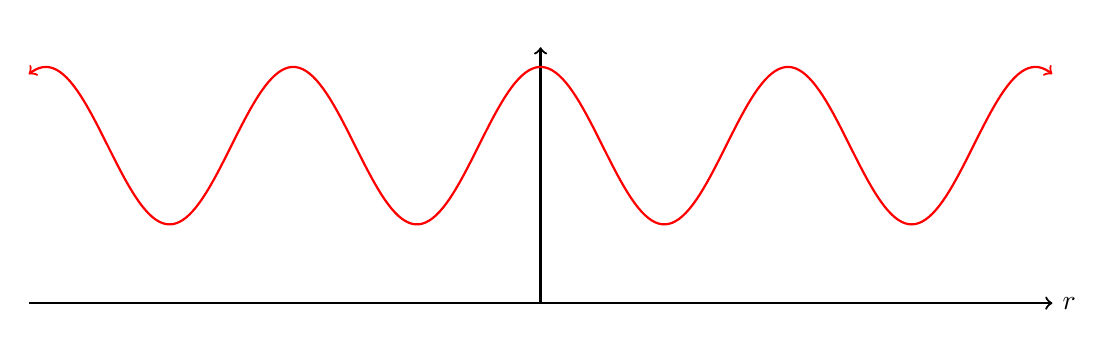
\begin{tikzpicture}[
	tl/.style = {% tick labels
		fill=white, inner sep=1pt, font=\scriptsize,},
	]
	
	% axes
	\draw[->,thick] (-6.5,-2) -- (6.5,-2) node[right] {$\vb{r}$};
	\draw[->,thick] (0,-2) -- (0, 1.25) node[above] {$$};
	% curve
	\draw[<->,thick,draw=red,
	domain=-6.5:6.5,samples=300,variable=\x] 
	plot (\x,{cos(deg{\x*2})});

\end{tikzpicture}

\begin{equation}
	H = \sum_i \left[\frac{\vb{P}_i^2}{2m} + U(\vb{r}_i)  \right]+ \sum_{ij} V_{e-e}^C (\vb{r}_i-\vb{R}j)
\end{equation}

\noindent This is, in general, a very hard problem to solve. In particular, it is the Coulomb-term which makes it really hard.\\
\linebreak

\noindent\uline{One-particle term:}
\begin{align}
	&H_1 = \sum_i H_1 (\vb{r}_i, \vb{P}_i)\\
	&H_1 (\vb{r}_i, \vb{P}_i) = \frac{\vb{P}_i^2}{2m} + U(\vb{r}_i)
\end{align}
\linebreak
\noindent \uline{Two-particle term:}
\begin{equation}
	H_2 = \sum_{ij} V_{e-e}^C (\vb{r}_i-\vb{R}j
\end{equation}

\noindent We will first work out the second-quantized form of the two terms in $H_1 (\vb{r}_i, \vb{P}_i)$. \\
\linebreak

\noindent We define $\varphi_\lambda ( \vb{r},s)$ as follows:
Solutions to the single-particle Schrödinger-equation

\begin{align}
	&H_1 \varphi_\lambda = \varepsilon_\lambda \varphi_\lambda\\
	&H_1 = -\frac{\hbar^2}{2m} \vb{\laplacian} + U(\vb{r}) ; \hspace{0.5cm} \vb{\laplacian} : \text{Laplace-operator} \label{h_1}
\end{align}

\noindent The task is now to find a second-quantized form of $H_1$ which will yield the \uline{same} matrix elements as \ref{h_1}.\\
\linebreak
\noindent Consider:
\begin{equation}
	\bra{\lambda_1} H_1 \ket{\lambda_2} ; \hspace{0.5cm} \braket{\lambda_1}{\lambda_2} = \delta_{\lambda_1, \lambda_2}
\end{equation}

\noindent \uline{Completeness relation:}

\begin{align}
	&\braket{\vb{r},s}{\lambda_1} = \varphi_{\lambda_{1}} \hspace{0.5cm} \text{(some wavefunction)} \nonumber\\
	&\text{Normalized states: } \braket{\lambda}{\lambda}=1 \nonumber \\
	&\sum_\lambda \varphi_\lambda^* (\vb{r},s) \varphi_\lambda (\vb{r'},s') = \delta(\vb{r}-\vb{r'}) \delta_{s,s'}\\
	&\sum_{\vb{r},s} \varphi_{\lambda'}^* (\vb{r},s) \varphi_\lambda (\vb{r},s) = \delta_{\lambda, \lambda'}\\
	& \braket{\lambda}{\lambda'}= \delta_{\lambda, \lambda'} \implies \sum_{\vb{r},s} \ket{\vb{r},s} \bra{\vb{r},s} = 1 ; \hspace{0.3cm} \sum_x \ket{x}\bra{x}=1
\end{align}

\noindent Now we use this version of the completeness relations to evaluate the matrix element $\bra{\lambda_1} H_1 \ket{\lambda_2}$

\begin{align}
	\bra{\lambda_1} H_1 \ket{\lambda_2} &= \sum_{\vb{r},s} \sum_{\vb{r'},s'} \braket{\lambda_1}{\vb{r},s} \bra{\vb{r},s} H_1 \ket*{\vb{r'},s'} \braket*{\vb{r'}}{\lambda_2}\\
	&=  \sum_{\vb{r},s} \sum_{\vb{r'},s'} \varphi_{\lambda_1}^* (\vb{r},s)  \bra{\vb{r},s} H_1 \ket*{\vb{r'},s'} \varphi_{\lambda_2} (\vb{r'},s') \nonumber
\end{align}

\begin{align}
	&H_1 = \frac{\vb{p}^2}{2m}+ U(\vb{r}) \hspace{1cm} \text{Classical}\\
	&\vb{p}= \frac{\hbar}{i} \vb{\gradient}  ;  \hspace{1cm} \vb{\gradient}: \text{Gradient operator}\\
	&H_1 =  - \frac{\hbar^2 \vb{\laplacian}}{2m} + U(\hat{r}) \hspace{1cm} \text{Quantum mechanical}\\
	& U(\hat{r}) \ket{r} = U(\vb{r})\ket{r}
\end{align}

\noindent $\vb{r}:$ Position : eigenvalue of the position operator

\begin{align}
	\hat{r} \ket{\vb{r},s}= \vb{r} \ket{\vb{r}, s}\\
	U(\hat{r}) \ket{\vb{r},s}= U(\vb{r}) \ket{\vb{r},s}
\end{align}


\begin{align}
	\bra{\vb{r},s} H_1 \ket*{\vb{r'},s'} &= \left[-\frac{\hbar^2}{2m} \vb{\laplacian}+ U(\vb{r}) \right] \delta_{\vb{r}, \vb{r'}} \delta_{s,s'}\\
	\bra{\lambda_1} H_1 \ket{\lambda_2} &= \sum_{\vb{r},s} \varphi_{\lambda_1}^* (\vb{r},s) \left[-\frac{\hbar^2}{2m} \vb{\laplacian}+ U(\vb{r}) \right] \varphi_{\lambda_2} (\vb{r},s)\\
	&\equiv \varepsilon_{\lambda_1, \lambda_2} \nonumber
\end{align}

\noindent $\varphi_\lambda (\vb{r},s): $ Some complete set of functions, by assumption.\\
\linebreak
\noindent Let us now give an alternative form of $H_1$, which will yield the \uline{same} matrix elements.
\linebreak
\noindent \uline{Anzats:}

\begin{equation}
	H_1 = \sum_{\lambda_1, \lambda_2} h_{\lambda_1, \lambda_2} \cd_{\lambda_1} c_{\lambda_2}
\end{equation}
where $ h_{\lambda_1, \lambda_2}$ is some complex number.
Then:
\begin{align}
	\bra{\lambda_1} H_1 \ket{\lambda_2} &= \bra{0}c_{\lambda_1} \left(\sum_{\lambda'_1, \lambda'_2} h_{\lambda'_1, \lambda'_2} \cd_{\lambda'_1} c_{\lambda'_2} \right) \cd_{\lambda_2} \ket{0} \\
	&=\sum_{\lambda'_1, \lambda'_2} h_{\lambda'_1, \lambda'_2}  \bra{0}c_{\lambda_1}  \cd_{\lambda'_1} c_{\lambda'_2} \cd_{\lambda_2} \ket{0} \nonumber \\
	&= \sum_{\lambda'_1, \lambda'_2} h_{\lambda'_1, \lambda'_2}  \bra{0} (\delta_{\lambda_1, \lambda'_1}-\cd_{\lambda'_1}c_{\lambda_1} ) (\delta_{\lambda_2, \lambda'_2} -\cd_{\lambda_2} c_{\lambda'_2}) \ket{0} \nonumber\\
	&= \sum_{\lambda'_1, \lambda'_2} h_{\lambda'_1, \lambda'_2}  \delta_{\lambda_1, \lambda'_1} \delta_{\lambda_2, \lambda'_2} \braket{0}{0}\nonumber \hspace{1cm} (c_\lambda \ket{0} =0)  \\
	&= h_{\lambda_1, \lambda_2} \nonumber
\end{align}
Choose $ h_{\lambda_1, \lambda_2} = \varepsilon_{\lambda_1, \lambda_2}$ $\implies$ Same matrix-elements for
\begin{equation}
	H_1 = -\frac{\hbar^2}{2m} \vb{\laplacian}+ U(\hat{r}) 
\end{equation}
and
\begin{tcolorbox}
	\begin{equation}
		H_1 = \sum_{\lambda_1, \lambda_2} \varepsilon_{\lambda_1, \lambda_2} \cd_{\lambda_1} c_{\lambda_2} \label{sec_quant_h}
	\end{equation}
\end{tcolorbox}
Thus, \ref{sec_quant_h} is a useful 2nd quantized form of $H_1$.\\
\linebreak
\noindent This expression may be simplified. Consider now a judicial choice of the complete set $\{\varphi_\lambda(x) \}$:\\
\noindent Let ${\varphi_\lambda}$ be defined by

\begin{equation}
	\left(-\frac{\hbar^2}{2m} \vb{\laplacian}+ U(\vb{r})  \right) \varphi_\lambda(x) = \varepsilon_\lambda \varphi_\lambda(x)
\end{equation}
i.e. ${\varphi_\lambda}$ are eigenfunctions of $H_1$\\
\linebreak
\noindent Then:
\begin{align}
	\varepsilon_{\lambda_1, \lambda_2} &= \sum_x \varphi_{\lambda_1}^*(x)  \left(-\frac{\hbar^2}{2m} \vb{\laplacian}+ U(\vb{r})  \right) \varphi_{\lambda_2} (x)\\
	&=  \sum_x \varphi_{\lambda_1}^*(x) \varepsilon_{\lambda_2} \varphi_{\lambda_2}(x) \nonumber \\
	&= \varepsilon_{\lambda_2} \sum_x \varphi_{\lambda_1}^*(x) \varphi_{\lambda_2}(x)\nonumber \\
	&= \varepsilon_{\lambda_2} \delta_{\lambda_1, \lambda_2} \nonumber
\end{align}
giving that, 
\begin{equation}
	H_1 = \sum_{\lambda_1} \varepsilon_{\lambda_1} \cd_{\lambda_1} c_{\lambda_1}
\end{equation}

\noindent This form of $H_1$ has an intuitively appealing form: $  \cd_{\lambda_1} c_{\lambda_1}$ is a number operator. It counts the number of particles in state $\ket{\lambda_1}$.\\
\noindent $\varepsilon_\lambda$ is the single-particle energy in this state. Thus, $H_1$ is an operator that counts the energy in the system coming from all the possible states of the system.\\
\linebreak
\noindent General one-particle operators:
\begin{equation}
	T(x, \vb{p}) = T(x, \frac{\hbar}{i} \vb{\gradient}) 
\end{equation}
Could in principle depend on spin-coordinate $s$ !
\begin{equation}
	\bra{\lambda_1} T \ket{\lambda_2} = \sum_x \varphi_{\lambda_1}^*(x) T(x, \frac{\hbar}{i} \vb{\gradient}) \varphi_{\lambda_2}(x)
\end{equation}

\begin{tcolorbox}
	\begin{align}
		T &= \sum_{\lambda_1,\lambda_2} \bra{\lambda_1} T(x, \vb{p}) \ket{\lambda_2} \cd_{\lambda_1} c_{\lambda_2}\\
		&=\sum_{\lambda_1,\lambda_2} t_{\lambda_1,\lambda_2} \cd_{\lambda_1} c_{\lambda_2} \nonumber
	\end{align}
\end{tcolorbox}
\noindent This expression for $H_1$ and $T$ in second quantized form applies for any choice of sets of quantum numbers $\lambda$.\\
\linebreak
\noindent We next proceed by setting up a general form of second quantized form of 2-particle operators.


\begin{equation}
	H= \sum_i H_1(\vb{p}_i, \vb{r}_i) + \sum_{i,j} H_2 (\vb{r}_i, \vb{r}_j )
\end{equation}

\begin{tcolorbox}
	\noindent Second-quantized form (general):
	
	\begin{align}
		H & = \sum_{\lambda_{1}, \lambda_{2}} \bra{\lambda_{1}} H_1 \ket{\lambda_{2}} \cd_{\lambda_1} c_{\lambda_2} \nonumber \\
		&+ \sum_{\lambda_{1}} \cdots \sum_{\lambda_{4}} \bra{\lambda_{1}, \lambda_{2}} H_2 \ket{\lambda_{3}, \lambda_{4}} \cd_{\lambda_1} \cd_{\lambda_2} c_{\lambda_{3}} c_{\lambda_{4}}
	\end{align}
\end{tcolorbox}
\linebreak

\subsection{Plane-wave basis}

\noindent i) \uline{Plane-wave basis:}  ${\varphi_{\lambda} (\vb{r},s) = \frac{1}{\sqrt{V}} \e^{i \vb{k}\cdot \vb{r}} \chi_\sigma (s)  }$ \\
\linebreak

\noindent \uline{Completeness:}

\begin{equation}
	\sum_{\vb{k}} \sum_{\sigma} \varphi_{\vb{k}, \sigma}^* (\vb{r}', s') \varphi_{\vb{k}, \sigma} (\vb{r}, s) = \delta_{\vb{r}, \vb{r}'} \delta_{s,s'}
\end{equation}
\linebreak
\noindent \uline{Orthogonality:}

\begin{equation}
	\sum_{\vb{r}} \sum_{s} \varphi_{\vb{k}', \sigma'}^* (\vb{r}, s) \varphi_{\vb{k}, \sigma} (\vb{r}, s) = \delta_{\vb{k}, \vb{k}'} \delta_{\sigma,\sigma'}
\end{equation}
\linebreak
\noindent Field-operators are given by

\begin{equation}
	\psi^\dagger (\vb{r},s,t) = \sum_{\vb{k}, \sigma} \cd_{\vb{k}, \sigma} (t) \left( \frac{1}{\sqrt{V}} \e^{i \vb{k} \cdot \vb{r}} \chi_\sigma (s) \right)
\end{equation}

\begin{align}
	&\{c_{k,\sigma}(t), \cd_{ k', \sigma'} \}= \delta_{k,k'}\delta_{\sigma,\sigma'}\\
	&\{c_{k,\sigma}(t), c_{ k', \sigma'} \}= 0\\
	&\{\cd_{k,\sigma}(t), \cd_{ k', \sigma'} \}= 0
\end{align}

\noindent Orthonormality, spatial part

\begin{equation}
	\frac{1}{V} \sum_{\vb{r}} \e^{i \vb{r}\cdot (\vb{k}-\vb{k}')} = \delta_{\vb{k}, \vb{k}'}
\end{equation}

\noindent Orthonormality, spin part

\begin{equation}
	\sum_s \chi_{\sigma_1}^* (s) \chi_{\sigma_2} (s) = \delta_{\sigma_1,\sigma_2}
\end{equation}

\noindent Completeness, spatial part

\begin{equation}
\frac{1}{V} \sum_{\vb{k}} \e^{i \vb{k}\cdot (\vb{r}-\vb{r}')} = \delta_{\vb{r}, \vb{r}'}
\end{equation}

\noindent Completeness, spin part

\begin{equation}
\sum_{\sigma} \chi_{\sigma}^* (s') \chi_{\sigma} (s) = \delta_{s',s}
\end{equation}

\noindent The plane-waves are eigenfunctions of $H_{10} \equiv -\frac{\hbar^2}{2m} \vb{\laplacian}$ $\implies$

\begin{align}
	& H_{10} = \sum_{\vb{k}_1, \sigma_1} \sum_{\vb{k}_2, \sigma_2} \bra*{\vb{k}_1, \sigma_1} H_{10} \ket*{\vb{k}_2, \sigma_2} \cd_{ \vb{k}_1, \sigma_1} c_{\vb{k}_2, \sigma_2}\\
	&  \bra*{\vb{k}_1, \sigma_1} H_{10} \ket*{\vb{k}_2, \sigma_2}  = \frac{1}{V} \sum_{\vb{r}} \e^{i (\vb{k}_1-\vb{k}_2)\cdot \vb{r}}  \sum_s \chi_{\sigma_1}^*(s) \chi_{\sigma_2}(s) \frac{\hbar^2 k_2^2}{2m}\\
	& H_{10}= \sum_{\vb{k_1}, \sigma_1} \frac{\hbar^2 k_1^2}{2m} \cd_{ \vb{k}_1, \sigma_1} c_{ \vb{k}_1, \sigma_1} \nonumber\\ 
	& H_{10}= \sum_{\vb{k}, \sigma} \varepsilon_k \cd_{k \sigma} c_{ k, \sigma} \hspace{0.1cm} ; \hspace{0.5cm} \varepsilon_k = \frac{\hbar^2 k^2}{2m} \nonumber
\end{align}

\noindent The next contribution to $H_1$ is the crystal potential $U(\vb{r}_i)= H_{11}(r_i)$\\
$ \sum_i U(\vb{r}_i) \rightarrow \sum_{\lambda_{1}, \lambda_{2}} \bra{\lambda_{1}}H_{11} \ket{\lambda_{2}} \cd_{ \vb{k}_1, \lambda_1} c_{\lambda_{2}}$

\begin{align}
	\bra{\lambda_{1}} H_{11} \ket{\lambda_{2}} &= \sum_{\vb{r}} \sum_s \frac{1}{\sqrt{V}} \e^{-i \vb{k}_1\cdot \vb{r}} \chi_{\sigma_1}^*(s) U(\vb{r}) \frac{1}{\sqrt{V}} \e^{i \vb{k}_2 \cdot \vb{r}} \chi_{\sigma_2}(s)\\
	&= \frac{1}{V} \sum_{\vb{r}} \e^{i (\vb{k}_2-\vb{k}_1) \cdot \vb{r}} U(\vb{r}) \sum_s \chi_{\sigma_1}^* (s) \chi_{\sigma_2}(s) \nonumber 
\end{align}

\noindent Introduce Fourier-transform of the crystal-potential

\begin{align}
	\tilde{U}(\vb{q}) &\equiv \frac{1}{V} \sum_{\vb{r}} \e^{-i \vb{q}\cdot \vb{r}} U(\vb{r})\\
	U(\vb{r}) &= \sum_{\vb{q}} \tilde{U}(\vb{q}) \e^{i \vb{q} \vb{r}}
\end{align}

\begin{equation}
	\bra{\lambda_{1}} H_{11} \ket{\lambda_{2}}= \delta_{\sigma_1,\sigma_2} \tilde{U}(\vb{k}_1-\vb{k}_2)
\end{equation}


\begin{align}
	\sum_{\lambda_{1}} \sum_{\lambda_{2}} 	\bra{\lambda_{1}} H_{11} \ket{\lambda_{2}} \cd_{\lambda_1} c_{\lambda_{2}} &= \sum_{\vb{k}_1} \sum_{\vb{k}_2} \sum_{\sigma} \tilde{U}(\vb{k}_1-\vb{k}_2) \cd_{ \vb{k}_1, \sigma} c_{\vb{k}_2, \sigma} \nonumber \\
	&= \sum_{\vb{k}, \vb{q}, \sigma} \tilde{U} (\vb{q}) \cd_{ \vb{k}+\vb{q}, \sigma} c_{\vb{k}, \sigma} \nonumber
\end{align}

\noindent Where we have defined $\vb{q} \equiv \vb{k}_1- \vb{k}_2$ ; $\vb{k}_2 \equiv \vb{k}$.\\
\linebreak
\noindent Scattering of plane-waves $\ket*{\vb{k}, \sigma} \rightarrow \ket*{\vb{k}+\vb{q}, \sigma}$ by crystal lattice. Momentum $\vb{q}$ is transferred to fermions (electrons) from the lattice. Spin is conserved in the scattering. 

\begin{align}
	H_1 &= \sum_i \left[ \frac{p_i^2}{2m}+U(\vb{r}_i) \right] \implies \\
	H_1 &= \sum_{\vb{k}, \sigma} \varepsilon_k \cd_{k, \sigma} c_{k, \sigma} +\sum_{\vb{k},\vb{q}, \sigma} \tilde{U}(\vb{q})  \cd_{ k+q, \sigma} c_{k,\sigma} \hspace{0.5cm} ; \hspace{0.2cm} \varepsilon_k= \frac{\hbar^2 k^2}{2m}
\end{align}


\begin{figure}[!h]
	\centering
		\begin{tikzpicture}%[scale=3]
			%\itshape
			\begin{feynman}[large]
				\vertex[small,dot](a){};
				\vertex [right= of a](b);
				\vertex [above left=of a](i1);
				\vertex [below left=of a](i2);
				
				\node[anchor = east] at ($(a)+(+0.1,0)$) ;
				\diagram{
				(b) --[scalar, edge label' = $\tilde{U}(\vb{q})$] (a) ,
				(i2)--[fermion, edge label' ={\(\vb{k}, \sigma\)}] (a) -- [fermion, edge label'={\(\vb{k}+\vb{q}, \sigma\)}] (i1), 	
				};
			\end{feynman}
	
		\end{tikzpicture}
	\caption*{Illustration of the scattering event}
\end{figure}

\noindent Next, we second-quantize the Coulomb interaction in the plane-wave basis.\\
\linebreak
\noindent Electron-electron interaction:


\begin{equation}
	H_2 = \sum_{\lambda_{1}}\cdots \sum_{\lambda_{4}} \bra{\lambda_{1}, \lambda_{2}}V_{e-e}^C \ket{\lambda_{3},\lambda_{4}} \cd_{\lambda_1} \cd_{\lambda_2} c_{\lambda_{3}} c_{\lambda_4}
\end{equation}

\begin{align}
	&\bra{\lambda_{1}, \lambda_{2}}V_{e-e}^C (\vb{r}_i-\vb{r}_j) \ket{\lambda_{3},\lambda_{4}} \\
	&= \sum_{s_1} \cdots \sum_{s_4} \chi_{\sigma_1}^* (s_1) \chi_{\sigma_2}^*(s_2) \chi_{\sigma_3}(s_3) \chi_{\sigma_4}(s_4) \nonumber\\
	& \cdot \frac{1}{V^2} \sum_{\vb{r}_1 \cdots \vb{r}_4} \e^{-i \vb{k}_1 \vb{r}_1- i \vb{k}_2 \cdot \vb{r}_2 + i \vb{k}_3\cdot \vb{r}_3+ i \vb{k}_4 \cdot \vb{r}_4  }  \nonumber \\ 
	& \cdot V_{e-e}^C (\vb{r}_3- \vb{r}_4) \delta_{s_2, s_3} \delta_{s_1, s_4} \delta_{\vb{r}_2, \vb{r}_3} \delta_{\vb{r}_1, \vb{r}_4}\nonumber 
\end{align}

\noindent Spin-part: Four sums over s's reduce to two:

\begin{equation*}
	\sum_{s_1} \sum_{s_2}  \chi_{\sigma_1}^* (s_1) \chi_{\sigma_2}^*(s_1) \chi_{\sigma_3}(s_2) \chi_{\sigma_4}(s_2) = \delta_{\sigma_1,\sigma_2} \delta_{\sigma_3, \sigma_4}
\end{equation*}

\noindent Spatial part: Again, four sums over $\vb{r}$ reduce to 2: 

\begin{equation*}
	\sum_{\vb{r}_1} \sum_{\vb{r}_2} V_{e-e}^C (\vb{r}_2-\vb{r}_1) \frac{1}{V^2} \e^{i (\vb{k}_4-\vb{k}_1)\cdot \vb{r}_1} \e^{i (\vb{k}_3-\vb{k}_2)\cdot \vb{r}_2} 
\end{equation*}
\noindent Rewrite plane-wave factors in such a way that we can factor out a Fourier-transform of $V_{e-e}^C (\vb{r}_2-\vb{r}_1)$. We therefore need a plane-wave factor of the type $\e^{i \vb{q}\cdot (\vb{r}_2- \vb{r}_1)}$. Since the spatial argument of $V_{e-e}^C$ is $\vb{r}_2 -\vb{r}_1$ here.

\begin{equation*}
	\e^{i (\vb{k}_4-\vb{k}_1)\cdot \vb{r}_1} \e^{i (\vb{k}_3-\vb{k}_2)\cdot \vb{r}_2}  = \e^{i(\vb{k}_4-\vb{k}_1+ \vb{k}_3-\vb{k}_2)\cdot \vb{r}_1} \e^{i(\vb{k}_3- \vb{k}_2) \cdot (\vb{r}_2- \vb{r}_1)}
\end{equation*}

\noindent Define $\vb{r}_2 -\vb{r}_1 \equiv \vb{r}$ and sum over $(\vb{r}, \vb{r}_1)$ instead of $(\vb{r}_1, \vb{r}_2)$

\begin{align*}
	\sum_{\vb{r}} V_{e-e}^C \e^{i(\vb{k}_3-\vb{k}_2)\cdot \vb{r}} \frac{1}{V^2} \sum_{\vb{r}_1} \e^{i(\vb{k}_3+\vb{k}_4-\vb{k}_1-\vb{k}_2)\cdot \vb{r}_1} &=\sum_{\vb{r}} V_{e-e}^C \e^{i(\vb{k}_3-\vb{k}_2)\cdot \vb{r}}   \frac{1}{V} \delta_{\vb{k}_3+\vb{k}_4, \vb{k}_1+\vb{k}_2}\\
	&= \tilde{V}_{e-e}^C (\vb{k}_2-\vb{k}_3) \delta_{\vb{k}_3+\vb{k}_4, \vb{k}_1+\vb{k}_2}
\end{align*}

\noindent Fourier-transform of Coulomb-potential: 

\begin{align*}
	\tilde{V}_{e-e}^C (\vb{q})  \equiv \frac{1}{V} \sum_{\vb{r}} \e^{-i \vb{q} \cdot \vb{r} } V_{e-e}^C (\vb{r})
\end{align*}


\noindent Thus, we have so far

\begin{align*}
	H_2 = \sum_{\vb{k}_1...\vb{k}_4 } \sum_{\sigma_1, \sigma_2} \tilde{V}_{e-e}^C (\vb{k}_2- \vb{k}_3) \delta_{\vb{k}_3+\vb{k}_4, \vb{k}_1+\vb{k}_2} \cd_{ \vb{k}_1, \sigma_1} \cd_{ \vb{k}_2, \sigma_2}  c_{ \vb{k}_3, \sigma_2} c_{ \vb{k}_4, \sigma_1},
\end{align*}

defining $\vb{q} \equiv \vb{k}_2- \vb{k}_3 \implies \vb{k}_3 =  \vb{k}_2-\vb{q}, \hspace{0.4cm} \vb{k}_4 = \vb{k}_1 + \vb{k}_2-\vb{k}_3 = \vb{k}_1- \vb{q}$.
Thus, sum over $\vb{k}_1, \vb{k}_2, \vb{q}$:

\begin{align*}
H_2 = \sum_{\vb{k}_1,\vb{k}_2,\vb{q} } \sum_{\sigma_1, \sigma_2} \tilde{V}_{e-e}^C (\vb{q}) \cd_{ \vb{k}_1, \sigma_1} \cd_{ \vb{k}_2, \sigma_2}  c_{ \vb{k}_3-\vb{q}, \sigma_2} c_{ \vb{k}_1+\vb{q}, \sigma_1}
\end{align*}

\noindent This is a scattering process between two electrons. 
\noindent Diagrammatically, we may view the scattering event as: 

 
\begin{center}
	\begin{tikzpicture}
	\begin{feynman}[large]
	\vertex (a); 
	\vertex[left= 3 cm of a] (b);
	\vertex[above left= 3cm of b] (c); 
	\vertex[below left= 3 cm of b] (d); 
	\vertex[above right= 3cm of a] (f1); 
	\vertex[below right= 3cm of a] (f2); 
	\diagram*{(b) --[charged boson, edge label = \(\vb{q}\)] (a), (b) --[fermion, edge label' = \( \vb{k}_1  \comma \sigma_1\)] (c), 
		(b) --[anti fermion, edge label = \(\vb{k}_1+\vb{q} \comma \sigma_1\)] (d), (a) --[fermion, edge label = \(\vb{k}_2 \comma \sigma_2\)] (f1), (a) --[anti fermion, edge label' = \(\vb{k}_2-\vb{q} \comma \sigma_2\)] (f2),
	}; 
	\node[anchor = west] at (-5,0) {};
	\node[anchor = west] at (0.2,0) {};
	\node[] at (-1.5,-0.6) {$\tilde{V}_{e-e}^C (\vb{q})$};
	\end{feynman}
	\end{tikzpicture}
\end{center}

\noindent Note that the spin of each electron is conserved in the scattering, since Coulomb-interaction is a purely electrostatic, spin-independent potential. This in total, we have

\begin{align*}
	H &= \sum_{\vb{k}, \sigma} \varepsilon_{\vb{k}} \cd_{ \vb{k}, \sigma} c_{\vb{k}, \sigma} +  \sum_{\vb{k}, \vb{q} \sigma} \tilde{U}(\vb{q}) \cd_{ \vb{k}+\vb{q}, \sigma}c_{\vb{k}, \sigma}\\
	& +  \sum_{\vb{k}_1,\vb{k}_2,\vb{q} } \sum_{\sigma_1, \sigma_2} \tilde{V}_{e-e}^C (\vb{q}) \cd_{ \vb{k}_1, \sigma_1} \cd_{ \vb{k}_2, \sigma_2}  c_{ \vb{k}_3-\vb{q}, \sigma_2} c_{ \vb{k}_1+\vb{q}, \sigma_1}
\end{align*}

\noindent For a static crystal, $\tilde{U}(\vb{q})$ is some given fixed external potential that electrons move in. In that case, it is the Coulomb term which makes the problem really hard, since it represents a genuine many-particle problem. On the other hand, if the lattice it self has dynamics, then this introduces additional scattering of electrons, now off quantized lattice vibrations (phonons). In that case, the second term involving $\tilde{U}(\vb{q})$ will include phonons, and this turns the $\tilde{U}(\vb{q})$- term also into a genuine many-body problem. We will later in the course return to the important problem of studying coupling between electrons and phonons.\newline

\subsection{Atomic orbital basis}

\noindent ii) \uline{Atomic orbital basis (lattice fermions)}

\noindent We now consider a system where fermions most of the time stay localized on sites on a lattice. Occasionally, they may tunnel from one lattice site to another. This tunneling arises because the long-distance (away from lattice sites) tails of the atomic orbitals (Wannier-functions) may overlap.

\begin{center}
	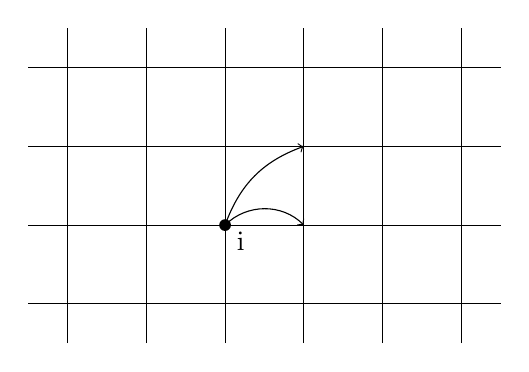
\begin{tikzpicture}
		\draw[step=1.0,black,thin] (0.5,0.5) grid (6.5,4.5);	
		\draw[->] (3,2)  to [out=70,in=200, looseness=1] (4,3);
		\draw[->] (3,2)  to [out=45,in=135, looseness=1] (4,2);
		\node at (3,2) [circle,fill,inner sep=1.5pt]{};
		\node at (3.2,1.8) {i};
	\end{tikzpicture}
\end{center}
\noindent Two tunneling processes ("hopping") on a 2D rectangular lattice, from lattice site \uline{i} to its \uline{nearest} and \uline{next-nearest} neighbors. The long distance tails of the Wannier-functions fall off exponentially (recall the wave-functions of the Hydrogen-atom). Therefore, hopping is most likely to occur from a lattice site i to its nearest neighbor. The next most probable hopping event is a direct hopping from i to its next-nearest neighbor, or two hopping via an intermediate nearest neighbor. Which process is most likely is a matter of some detail: The two factors that mostly determine this is the distance between atoms on the lattice, and the type of atoms which are situated on the lattice points. If $\Delta \vb{r}$ is the separation between the electron and the ionic position, then the Wannier-functions fall off approximatly as $\e^{-\Delta \vb{r}/\lambda}$
\begin{align*}
	\lambda = c \frac{a_0}{Z}
\end{align*}

\noindent $c$: Constant of order unity \newline
\noindent $a_0$: Bohr-radius\newline
\noindent $Z$: Number of protons in the nucleus\newline

\noindent For heavy atoms, Wannier orbitals are more tightly localized around atoms than in lighter elements. \newline
Crystal potential (rigid crystal) \newline

\noindent $U= \sum_i U(\vb{r}_i) $ \\
\noindent $U(\vb{r}_i)= \sum_j U(\vb{r}_i, \vb{R}j)$\\
\noindent $\vb{r}_i$: Electronic coordinate ; $\vb{R}j$: Ionic coordinate.\\

\noindent $U_a(\vb{r}_i, \vb{R}j)$: Potential energy that electron at $\vb{r}_i$ feels from ion located at $\vb{R}j$. The dominant contribution to this is when $i=j$, i.e. when the electron and ion is on the same site $i$. We single out this contribution as follows
\begin{align*}
	U = \sum_i U_a(\vb{r}_i, \vb{r}_i) + \sum_i \sum_{j\neq i}  U_a(\vb{r}_i, \vb{R}j).
\end{align*}
\noindent The point of this splitting is that the basis functions $\{\varphi_\lambda \}$ that we will choose, will be the eigenfunctions of the total Hamilton-operator for \uline{isolated} atoms. This is a very natural choice for a system where electrons spend most of the time on isolated atoms and only relatively rarely hop from one site to the other.\newline

\noindent Schrödinger-equation for isolated atoms:

\begin{align*}
	\left[\frac{\vb{p}_i^2}{2m}+ U_a( \vb{r}_i, \vb{R}_i)\right] \varphi_{\alpha, \sigma}( \vb{r}_i, s_i)= \varepsilon_{\alpha,\sigma, i} \varphi_{\alpha, \sigma}( \vb{r}_i, s_i)
\end{align*}

\noindent $\alpha$: Index for atomic orbital \\
\noindent $\sigma$: Spin quantum number\\
\noindent $\vb{r}_i$: Spatial coordinate of electron on lattice site $i$\\
\noindent $\s_i$: Spin-coordinate of electron on lattice site $i$r\\
\noindent $\varepsilon_{\alpha,\sigma, i}$: Energy of electron in orbital $\alpha$ on lattice site$i$. In principle this energy could vary from lattice site to lattice site, but for most systems we will let $\varepsilon_{\alpha, \sigma, i} = \varepsilon_{\alpha, \sigma}$ i.e. independent of the position on the lattice. In principle, $\varepsilon_{\alpha, \sigma}$ could depend on spin. 
If we now bring in the rest of the crystal potential (from the surrounding atoms) in the one-particle Hamiltonian, the basis set $\{\varphi_\lambda \}$ that we have chosen, are no longer eigenfunctions of the Hamiltonian. This leads to scattering from one state $\ket{\lambda}$ to another state $\ket{\lambda'}$, and this in term gives rise to tunneling, or hopping, of electrons on the lattice. Thus, the hopping of electrons around on the lattice, which represents kinetic energy, originates with the crystal potential from surrounding atoms working on an electron. The details are as follows:

\begin{align*}
	&\varphi_{\alpha, \sigma,j}(\vb{r}_i,s_i) = \Phi_{\alpha, j}^W (\vb{r}_i) \cdot \chi_\sigma (s_i)\\
	&\lambda = (\alpha, \sigma, j)
\end{align*}
(\uline{Note}: $\alpha$ must be thought of as consisting of two numbers: (l,m) of a hydrogen-like atom.)\\

\noindent Field operator:
\begin{align*}
	\psi^\dagger_j(\vb{r}_i, s_i, t)= \sum_{\alpha, \sigma} \cd_{\alpha, \sigma, i} \Phi_{\alpha, j}^* (\vb{r}_i) \cdot \chi^*_\sigma (s_i)
\end{align*}
\begin{align*}
	\{ c_{\alpha, \sigma, i},\cd_{\alpha', \sigma', i'} \} = \delta_{\alpha, \alpha'} \delta_{\sigma,\sigma'} \delta_{i,i'}
\end{align*}
Other commutators are zero.\\

\noindent \uline{Orthogonality}:

\begin{align*}
	\sum_{\vb{r}} \sum_s  \varphi^*_{\alpha, \sigma,j}(\vb{r},s)\varphi_{\alpha', \sigma',j'}(\vb{r},s) \approx \delta_{\alpha, \alpha'} \delta_{\sigma,\sigma'} \delta_{j,j'}
\end{align*}

\noindent \uline{Completeness}:

\begin{align*}
\sum_{\alpha, \sigma, j} \varphi^*_{\alpha, \sigma,j}(\vb{r},s)\varphi_{\alpha, \sigma,j}(\vb{r}',s') \approx \delta_{\vb{r},\vb{r}'} \delta_{s,s'} 
\end{align*}

\begin{align*}
	H_1 = \sum_j \left( \frac{\vb{p}_i^2}{2m}+ U_a (\vb{r}_i, \vb{R}_i) \right) + \sum_i \sum_{j \neq i} U_a ( \vb{r}_i, \vb{R}_j)
\end{align*} % 7-25  og hele Week 2 ? 
	% Week 3
	% Week 4
	\chapter{Temporary chapter name}
\suggestion{Suggestion for chapter name: ``Bosons: magnetic insulators and quantized lattice vibrations''}
\section{From the Hubbard-model to the quantum antiferromagnetic Heisenberg model}

We now return to the Hubbard model and consider this in a special, but important, limit.\\

\emph{The general staring point is:}
\begin{align}
\begin{split}
    \Ha &= \sum_{\lambda_1,\lambda_2} \mel{\lambda_1}{\Ha_1}{\lambda_2}c_{\lambda_1}^{\dagger} c_{\lambda_2} \\
    &+ \sum_{\substack{\lambda_1, \lambda_2, \\
    \lambda_3, \lambda_4}} \mel{\lambda_1 \lambda_2}{\Ha_2}{\lambda_3 \lambda_4}c_{\lambda_1}^\dagger c_{\lambda_2}^\dagger c_{\lambda_3} c_{\lambda_4}
\end{split}
\end{align}

\emph{Lattice fermions:}
\begin{enumerate}[i)]
    \item One type of fermions
    \item Lattice translational invariance (discrete)
    \item One orbital pr. site and at most two fermions pr. site \\

Under such circumstances the Hamiltonian takes the form:
\begin{equation}
    \Ha = - \sum_{i, j, \sigma} t_{ij} c_{i\sigma}^\dagger c_{j\sigma} \ + \sum_{\substack{i_1, i_2, i_3, i_4 \\ \sigma_1, \sigma_2}} \mel{i_1 i_2}{V}{i_3 i_4} \cdot c_{i_1\sigma_1}^\dagger c_{i_2\sigma_2}^\dagger c_{i_3\sigma_3} c_{i_4\sigma_4}
\end{equation}

\hspace{-0.5cm} \emph{Further simplifications}

\item Nearest-neighbor hopping only ($t_{ij} = t$)

\item Hubbard interaction only ($i_1 = i_2 = i_3 = i_4, V_{iiii} = U$)

\item \boxed{U/t \gg 1} NB!! \\

This gives:

\begin{align}
    \Ha &= -t \sum_{\substack{\langle i,j \rangle \\ \sigma}} c_{i\sigma}^\dagger c_{j\sigma} + U \sum_{i, \sigma} n_{i, \sigma} n_{i, -\sigma} \\
    n_{i\sigma} &= c_{i\sigma}^\dagger c_{i\sigma}
\end{align}

The Hubbard model, as written above, is valid for arbitrary ratio $U/t$, but we will consider it in the case $U/t \gg 1 $, where the fermions are said to be strongly correlated.

\item We now study the model at half-filling. That is, the number of fermions on the lattice is $N$, where $N$ is the \# of lattice points. On average, there is one fermion pr. lattice site. The lattice is therefore half-filled, since the maximum \# fermions on the lattice is $2N$. \\
\end{enumerate}


Since $U/t \gg 1$, we regard the unperturbed Hamiltonian $\Ha_0$ to be

\begin{equation}
    \Ha_0 = U\sum_{i, \sigma} n_{i \sigma} n_{i -\sigma}
\end{equation}

 This problem is easy to solve exactly, since it is completely local (it can be solved for each site independently).\\

 We will regard the hopping term as a perturbation. \\

Unperturbed ground state:
\begin{equation}
    \Ha_0 \ket{\psi_0} = E_0 \ket{\psi_0}
\end{equation}

\begin{description}
    \item $E_0 = 0$
    \item $\ket{\psi_0}$: One fermion on each lattice site. Massively degenerate, since the distribution of $\uparrow$ and $\downarrow$ does not matter.

    \item $N_f = N_{f \uparrow} + N_{f \downarrow} = N $
    \item $N_{f \uparrow} = N_{f \downarrow} = N/2$
    
    \item $N_f$: \# fermions
    \item $N_{f\uparrow}$: \# fermions with spin $\uparrow$
    \item $N_{f\downarrow}$: \# fermions with spin $\downarrow$

    \item $\ket{\psi_0}$: linear combination of states like $\ket{\uparrow\uparrow\downarrow\downarrow\uparrow\downarrow
    \uparrow...}$ with equally many $\uparrow \rm{and} \downarrow$.
\end{description}

There are $2^N$ such states. From degenerate perturbation theory: Find specifi linear combination of these $2^N$ states that changes \emph{little} when perturbation is introduced. Imagine that we have found this. Call this state $\ket{\psi_0}$ from now on.

\begin{equation}
    \Ha_{\text{hop}} = - \sum_{\substack{\langle i, j \rangle \\ \sigma}} t_{ij} c_{i\sigma}^\dagger c_{j\sigma}: \qquad \text{Perturbation.}
\end{equation}

\emph{1. order correction to $E_0$}:
\begin{align}
    \Delta E^{(1)} &= \mel{\psi_0}{\Ha_{\text{hop}}}{\psi_0} \\
    &= - \sum_{\substack{\langle i, j \rangle \\ \sigma}} t_{ij} \mel{\psi_0}{c_{i\sigma}^\dagger c_{j\sigma}}{\psi_0}
\end{align}

 $c_{i\sigma}^\dagger c_{j\sigma}\ket{{\psi_0}}$: A state where $i$ is double occupied and $j$ is unoccupied. This new state is orthogonal to $\ket{\psi_0} \implies \Delta E^{(1)} = 0$. \\

\emph{2. order correction to $E_0$}:
\begin{equation}
    \Delta E^{(2)} = \frac{\mel{\psi_0}{\Ha_{\text{hop}}}{n} \mel{n}{\Ha_{\text{hop}}}{\psi_0}}{E_0 - E_n}
\end{equation}

$\ket{n}$: Some intermediate excited eigenstate of $\Ha_0$:

\begin{equation}
    \Ha_0\ket{n} = E_n\ket{n}.
\end{equation}

Which $\ket{n}$ will contribute to $\Delta E^{(2)}$? They must be such that

\begin{align}
    \mel{\psi_0}{\Ha_{\text{hop}}}{n} &\ne 0 \\
    - \sum_{\substack{\langle i, j \rangle \\ \sigma}} t_{ij} \mel{\psi_0}{c_{i\sigma}^\dagger c_{j\sigma}}{n} & \ne 0 \\
    c_{i \sigma}^\dagger c_{j \sigma}\ket{n} & \sim \ket{\psi_0}
\end{align}

This means that $\ket{n}$ has to be a state with site $j$ doubly occupied and site $i$ unoccupied, thus $E_n = U + E_0 = U$.\\

Hence:
\begin{align}
    \Delta E^{(2)} &= -\frac{1}{U}\sum_n \mel{\psi_0}{\Ha_{\text{hop}}}{n}\mel{n}{\Ha_{\text{hop}}}{\psi_0} \\
    &= -\frac{1}{U} \mel{\psi_0}{\Ha_{\text{hop}}^2}{\psi_0}
\end{align}

Thus, $\Delta E^{(2)}$ is equivalent to a first-order correction to $E_0$ from an effective Hamiltonian

\begin{equation}
    \Ha_{\text{eff}} = -\frac{1}{U} \Ha_{\text{hop}}^2
\end{equation}

Since $\Ha_{\text{eff}}$  is the product of two one-particle Hamiltonians, it is in fact a two-particle Hamiltonian. Let us consider this in some more detail.

\begin{equation}
    \Ha_{\text{eff}} = -\frac{1}{U} \sum_{\langle i, j \rangle, \sigma}  \sum_{\langle l, k \rangle , \sigma'} t_{ij} t_{lk} \ c_{i \sigma}^\dagger c_{j \sigma}^{} \ c_{l \sigma'}^\dagger c_{k \sigma'}^{}
\end{equation}

A non-zero correction to the ground-state requires certain restrictions on $(i, j) \ \text{and} \ (l,k)$. Namely, \emph{after} $c_{i \sigma}^\dagger c_{j \sigma}^{} \ c_{l \sigma'}^\dagger c_{k \sigma'}^{}$ has acted on $\ket{\psi_0}$, the resulting state must $\sim \ket{\psi_0}$,

\begin{equation}
    c_{i \sigma}^\dagger c_{j \sigma}^{} \ c_{l \sigma'}^\dagger c_{k \sigma'}^{} \ket{\psi_0} \sim \ket{\psi_0}.
\end{equation}

\emph{In general:}
\begin{center}
	\begin{tikzpicture}
	
	\def\l{2};
	
	\coordinate (O) at (0,0);
	\coordinate (i) at (0.5*\l,0);
	\coordinate (j) at ($(i) + (\l,0)$);
	\coordinate (k) at ($ (j) + (\l,0) $);
	\coordinate (l) at ($(k) + (\l,0)$);
	\coordinate (R) at ($(l) + (0.5*\l,0)$);
	
	\draw[thick] (O) -- (R);
	
	\node[mark size=3pt,] at (i) {\pgfuseplotmark{x}};		
	\node[mark size=3pt,] at (j) {\pgfuseplotmark{x}};
	\node[mark size=3pt,] at (k) {\pgfuseplotmark{x}};
	\node[mark size=3pt,] at (l) {\pgfuseplotmark{x}};
	
	\draw[thick,->-=0.6] (j) to [out = 140, in=40] node[midway,above] {$\sigma$} (i);
	\draw[thick,->-=0.6] (k) to [in = 140, out=40] node[midway,above] {$\sigma'$} (l);
	
	\node[below=0.3cm] at (i) {$i$};
	\node[below=0.3cm] at (j) {$j$};	
	\node[below=0.3cm] at (k) {$k$};
	\node[below=0.3cm] at (l) {$l$};	
	
\end{tikzpicture}
\end{center}
\begin{gather}
    \mel{\psi_0}{\Ha_{\text{hop}}^2}{\psi_0} \ne 0 \quad \text{requires} \\
    i = k, \quad l = j \implies t_{ij}t_{lk} \rightarrow t_{ij}t_{ji} = t_{ij}t_{ij}^* = \abs{t_{ij}}^2 \geq 0
\end{gather}

That is, two fermions (one with spin $\sigma$, the other with spin $\sigma'$) is swapped between sites $i$ and $j$ 

\begin{center}
		\begin{tikzpicture}
	
	\def\l{2};
	
	\coordinate (O) at (0,0);
	\coordinate (i) at (0.5*\l,0);
	\coordinate (j) at ($(i) + (\l,0)$);
	
	\coordinate (R) at ($(j) + (0.5*\l,0)$);
	
	\draw[thick] (O) -- (R);
	
	\node[mark size=3pt,] at (i) {\pgfuseplotmark{x}};		
	\node[mark size=3pt,] at (j) {\pgfuseplotmark{x}};
	
	
	\draw[thick,->-=0.6] (j) to [out = 140, in=40] node[midway,above] {$\sigma$} (i);
	\draw[thick,->-=0.6] (i) to [in = 220, out=-40] node[midway,below] {$\sigma'$} (j);
	
	\node[below=0.3cm] at (i) {$i$};
	\node[below=0.3cm] at (j) {$j$};	
	
	
\end{tikzpicture}

\end{center}
This process is an \emph{exchange-process}.

Now, we have
\begin{align}
    \Ha_{\text{eff}} &= -\frac{1}{U} \sum_{\substack{i, j \\ \sigma, \sigma'}} \abs{t_{ij}}^2 c_{i \sigma}^\dagger c_{j \sigma}^{} c_{j \sigma'}^\dagger c_{i \sigma'} \\
    &= -\frac{1}{U} \sum_{\substack{i, j \\ \sigma, \sigma'}} \abs{t_{ij}}^2 c_{i \sigma}^\dagger c_{i \sigma'}^{} (\delta_{\sigma \sigma'} - c_{j \sigma'}^\dagger c_{j \sigma}^{})
\end{align}

The first term just contributes to the single-site energy. Absorb the first in the site-energy. \\

The remaining term is then \begin{equation}
    \Ha_{\text{eff}} = \frac{1}{U} \sum_{\substack{\langle i, j \rangle \\ \sigma, \sigma'}} \abs{t_{ij}}^2 c_{i \sigma}^\dagger c_{i \sigma'}^{} c_{j \sigma'}^\dagger c_{j \sigma}^{}
\end{equation}

Such an operator, we have already studied, and we know that, apart from an additive constant which we absorb in a reference zero-point of energy, it may be written as a spin-spin interaction

\begin{equation}
    \Ha_{\text{eff}} = \frac{4}{\hbar^2 U} \frac{1}{2} \sum_{i, j} \abs{t_{ij}}^2 \vb{S}_i \cdot \vb{S}_j
\end{equation}

where $\vb{S}_i = (S_{ix}, S_{iy}, S_{iz})$ are spin-operators $\vb{S} = \frac{\hbar}{2} \bm{\sigma}$. \\

$\bm{\sigma} = (\sigma_x, \sigma_y, \sigma_z)$ : Pauli-matrices (SU(2)-matrices: 2x2 unitary matrices with determinant = 1)

\begin{equation}
    \comm{S_{ix}}{S_{jy}} = i\frac{\hbar}{2}S_{iz}\delta_{ij} \ \text{etc: Quantum spins}.
\end{equation}

\begin{equation}
    \text{Define} \quad J_{ij} \equiv - \frac{2 \abs{t_{ij}}^2}{\hbar^2 U} < \ 0
\end{equation}

\begin{equation} \emph{
    \Ha_{\text{eff}} = -\sum_{\langle i, j \rangle} J_{ij} \vb{S_i} \cdot \vb{S_j}}
\end{equation}

 Since $J_{ij} < 0$ in this case, it favors spins that are \emph{anti-parallell on neighboring lattice sites}. This hints at the existence of antiferromagnetism in such strongly correlated fermion-systems, at least close to half-filling. \\

$\Ha_{\text{eff}}$ should be regarded as the effective low-energy Hamiltonian of the Hubbard-model in the \emph{strong-coupling limit $U/t \gg 1$}, at \emph{half-filling}. There are \emph{no terms} in $\Ha_{\text{eff}}$ that describes single-particle hopping processes on the lattice. There are \emph{no itinerant} fermions in this low-energy model. It therefore describes a quantum antiferromagnetic \emph{insulator}. The crucial feature that contributes to this fact, is that the system is assumed to be at 1/2-filling. \\

Let us also give a heuristic argument for why the Hubbard model, at 1/2-filling in the strongly coupled regime, gives rise to antiferromagnetism. \\

Localizing electrons on individual sites means that their wavefunctions are packed together tightly around the sites. Thus, they must contain many Fourier-components. This costs much kinetic energy. To lower this energy, it is advantageous to spread the wavefunctions out in space. This is facilitated by hopping to neighboring sites. To facilitate hopping, this means that spins on neighboring sites must have opposite spins (recall that we are at 1/2-filling). Therefore, antiferromagnetic order will facilitate this hopping to a maximum extent.

\begin{itemize}
    \item Coulomb interactions give rise to ferromagnetism (Hund's rule)
    
    \item Kinetic energy gives rise to antiferromagnetism
\end{itemize}

\begin{tcolorbox}
It is a matter of \emph{detail} which effect will dominate, and this explains the existence of ferromagnetism in some compounds, and antiferromagnetism in other compounds
\end{tcolorbox}

\begin{align}
    \Ha &= -\sum_{i, j} J_{ij}^{\text{tot}} \vb{S_i} \cdot \vb{S_j} \\
    J_{ij}^{\text{tot}} &= - \frac{2\abs{t_{ij}}^2}{U} + A\sum_{\vb{k}}\frac{\abs{I_{ij}}^2}{k^2} \\
    I_{jk}(\vb{k}) &= \sum_{\vb{r}}\phi_i^*(\vb{r})\phi_j(\vb{r}) e^{i\vb{k} \cdot \vb{r}} \\
A &= \frac{e^2}{\Omega_d \varepsilon_0}
\end{align}

	\section{2nd quantization for bosons}

Setting up a second-quantized version of a Hamiltonian for \underline{bosons} follows much of the same path as for fermions. Again, we define creation and destruction operators for states with q.n.'s $\lambda$

\begin{align}
    a_\lambda^\dagger \ket{0} &= \ket{\lambda} \quad ; \ a_\lambda\ket{n_\lambda} \sim \ket{n_\lambda - 1} \\
    (a_\lambda^\dagger)^{n_\lambda} &\sim \ket{n_\lambda} \ ; \ a_\lambda\ket{0} = 0
\end{align}

Main difference from fermions: it is allowed to occupy a single-particle state with an arbitrary number of particles. \\  Commutiation relations:

\begin{align}
    \comm{a_\lambda}{a_{\lambda'}^\dagger} &= \delta_{\lambda \lambda'} \\
    \comm\Big{a_\lambda}{a_{\lambda'}} &= 0 \\
    \comm{a_\lambda^\dagger}{a_{\lambda'}^\dagger} &= 0 \\ 
    (\comm{A}{B} &\equiv AB - BA)
\end{align}

 \uline{Field operator}:

\begin{align}
    \begin{rcases}
    A^\dagger (x, t) &= \sum_\lambda a_\lambda^\dagger \varphi_\lambda^*(x) \quad \\
    A(x, t) &= \sum_\lambda a_\lambda \varphi_\lambda(x)
    \end{rcases}
    \quad
    \comm{A(x,t)}{A^\dagger (x', t)} = \delta_{x, x'}
\end{align}

 $\{\varphi_\lambda(x)\}$: Complete set of functions which may be chosen conveniently, precisely as in the fermionic case. \\

 The general form of the Hamiltonian is identical in form to the fermionic case:

\begin{tcolorbox}
    \begin{align}
        \Ha &= \sum_{\lambda_1, \lambda_2} \varepsilon_{\lambda_1, \lambda_2}^{} a_{\lambda_1}^\dagger a_{\lambda_2}^\dagger
        + \sum_{\lambda_1, ..., \lambda_4}V_{\lambda_1 ... \lambda_4}^{}a_{\lambda_1}^\dagger a_{\lambda_2}^\dagger a_{\lambda_3}^{} a_{\lambda_4}^{}
    \end{align}
\end{tcolorbox}

NB!! The above form holds for bosons that are material particles, for instance Helium-4 atoms or cold-atom systems such as $\text{Rb}^{87}$. Bosons could also be non-material and interacting. An example would be quantized lattice vibrations, i.e. \uline{phonons}. For such systems, one could have interaction terms with an unequal number of creation and destruction operators. Such interaction terms do not conserve number of particles (Examples of this would be quantized anharmonic lattice vibrations, or quantum spin-fluctuations beyond linear spin-wave theory. We will consider such cases in the following). \\

An important application of this will be in studying quantized lattice vibrations and how they couple to electrons. Another important application is in the study of the low-temp. properties of quantum spin-systems. \\

\subsection{Low temperature properties of magnetic insulators}

We will consider fluctuation effects in quantum spin models of localized spins, i.e. magnetic insulators. In order to do this, we will consider spin-fluctuations that are small around some ordere state. Under such circumstances, we may find convenient representations of \uline{spin-operators} in terms of \uline{boson-operators}. \\

We will consider two main cases:
\begin{enumerate}[i)]
    \item \uline{Ferromagnetic insulators} described by a Hamiltonian
    \begin{equation}
        \Ha = -\sum_{i, j} J_{ij} \Vec{S_i}\cdot\Vec{S_j}, \quad J_{ij} > 0
    \end{equation}
    with a ground state where spins are ordered in parallell to each other. For the most part, we consider nearest-neighbor interactions.
    \item \uline{Antiferromagnetic insulators on a biparticle lattice}, described by
    \begin{equation}
        \Ha = -\sum_{i, j} J_{ij} \Vec{S_i}\cdot\Vec{S_j}, \quad J_{ij} < 0
    \end{equation}
    with a classical ground state where spins are ordered oppositely on neighboring lattice points. A simple biparticle lattice would be a 2D square lattice or a 3D cubic lattice. Again, for the most part, we consider nearest-neighbor spin-spin interactions. Including longer range interactions is no essential complication.
\end{enumerate}

The spin-operators for $S = 1/2$ spins satisfy the following commutation relations:
\begin{equation}
    \comm{S_{ix}}{S_{jy}} = i\hbar S_{iz}\delta_{ij}
\end{equation}
+ cyclic permutations, which may be written more compactly as
\begin{equation}
    \comm{S_{i\alpha}}{S_{j\beta}} = i\hbar \varepsilon_{\alpha\beta\gamma} \delta_{j\gamma} \delta_{ij} \\
\end{equation}
$(\alpha, \beta, \gamma) \in (x, y, z)  \text{ and } \varepsilon_{\alpha\beta\gamma}$ is the totally anti-symmetric tensor (Levi-Civita tensor). We will set $\hbar = 1$ in the following. \\

\subsubsection{Ferromagnetic case}
We assume that all spins are nearly completely ordered along the $z$-axis, and will introduce a boson-operator representation of the spins under this assumption. This representation must give correct commutation relations for spins.

\begin{equation}
    S_{iz} = S - a_i^\dagger a_i^{}, \quad S = 1/2
\end{equation}
Introduce $S_{i\pm} = S_{ix} \pm iS_{iy}$. These are spin-flip operators
\begin{align}
    &S_+ \ket{\downarrow} = \ket{\uparrow} \\
    &S_- \ket{\uparrow} = \ket{\downarrow} \\
    S_{i+} &= \sqrt{2S}(1-\frac{a_i^\dagger a_i^{}}{2S})^{1/2}a_i \\
    S_{i-} &= \sqrt{2S}(1-\frac{a_i^\dagger a_i^{}}{2S})^{1/2}a_i^\dagger = (S_{i+})^\dagger
\end{align}

The assumption of nearly-ordered spins is equivalent to the statement that we can approximate the boson-representation of spins by ignoring all terms beyond quadratic order in boson-operators.

\begin{align}
& \ \ S_{iz} = S - a_i^\dagger a_i^{} \\
&\begin{array}{c}
S_{i+} \approx \sqrt{2S}a_i \\
S_{i-} \approx \sqrt{2S}a_i^\dagger \\
\end{array}
\begin{cases}
\text{corrections to this involve cubic terms in } a, a^\dagger 
\end{cases}
\end{align}

$(a, a^\dagger)$: Satisfy boson comm. relations. Consider the nearest-neighbor case.

\begin{align}
    \Ha &= -J\sum_{\langle i,j \rangle} \Vec{S_i}\cdot\Vec{S_j} \\
    &= -J\sum_{\langle i, j \rangle}[S_{iz}S_{jz} + S_{ix}S_{jx} + S_{iy}S_{jy}]\\
    &= -J\sum_{\langle i, j \rangle}[S_{iz}S_{jz} + S_{i+}S_{j-}] \\
    &\approx -J\sum_{\langle i, j \rangle}[(S-a_i^\dagger a_i^{})(S-a_j^\dagger a_j^{}) + 2S a_i^{} a_j^\dagger]\\
    &\approx -J\sum_{\langle i, j \rangle}[S^2 - S(a_i^\dagger a_i^{} + a_j^\dagger a_j^{}) + 2S a_j^\dagger a_i^{}]
\end{align}

With \uline{no} spin-fluctuations present, we ignore terms involving boson-operators. In that case 
\begin{equation}
    \Ha = -J \sum_{\langle i, j \rangle} S^2
\end{equation}
which is simply the ground-state energy. Let us denote it by $E_0$, and use it as our reference energy ($E_0 \rightarrow 0$). Thus, we consider only the fluctuation part of the Hamiltonian from now.

\begin{equation}
    \Ha = 2SJ\sum_{\langle i, j \rangle} (a_i^\dagger a_i^{} - a_i^\dagger a_j^{}); \ J > 0
\end{equation}
\textcolor{red}{FIGUR: nearest-neighbor hopping}

\begin{align}
    a_i^\dagger &= \frac{1}{\sqrt{N}}\sum_{\Vec{k}}a_k^\dagger e^{i\Vec{k}\cdot\Vec{r_i}} \\
    a_i &= \frac{1}{\sqrt{N}}\sum_{\Vec{k}}a_k e^{-i\Vec{k}\cdot\Vec{r_i}}
\end{align}

We must next insert these representations into $\Ha. \ (a, a^\dagger)$ destroy and create quantized spin-fluctuations: \uline{magnons}.

\begin{align}
    \sum_{\langle i, j \rangle} a_i^\dagger a_j^{}
    &= \sum_{\Vec{r_i}}\sum_{\Vec{\delta}} \frac{1}{N}\sum_{\Vec{k_1}}\sum_{\Vec{k_2}}a_{k_1}^\dagger e^{i\Vec{k_1}\Vec{r_i}} a_{k_2} e^{-i\Vec{k_2}\Vec{r_j}} \\
    &= \frac{1}{N}\sum_{\Vec{k_1}}\sum_{\Vec{k_2}}a_{k_1}^\dagger a_{k_2} \underbrace{\sum_{\Vec{r_i}}e^{i(\Vec{k_1} - \Vec{k_2})\cdot\Vec{r_i}}}_{= N \delta_{\Vec{k_1}, \Vec{k_2}}} \underbrace{\sum_{\Vec{\delta}}e^{-i\Vec{k_2}\cdot \Vec{\delta}}}_{\equiv\gamma(\Vec{k_2})} \\
    &= \sum_{\Vec{k}}\gamma(\Vec{k})a_k^\dagger a_k^{}
\end{align}

\begin{equation}
    \sum_{\langle i, j \rangle} a_i^\dagger a_i^{} = z\sum_{\Vec{k}}a_k^\dagger a_k^{}
\end{equation}

\begin{align}
    \Ha &= 2SJ\sum_{\Vec{k}}[z-\gamma(\Vec{k})]a_k^\dagger a_k^{} \\
    &= \uline{\uline{\sum_{\Vec{k}}\omega_k a_k^\dagger a_k^{}}} \implies \text{Non-interacting Boson-gas}\\
    \omega_k &= \uline{\uline{2SJ(z-\gamma(\Vec{k}))}} \quad \text{Determined by J and lattice structure} \\
    z &= \# \text{ vectors } \Vec{\delta} \text{ included in } \gamma(\Vec{k}).
\end{align}

\begin{align}
    \gamma(\Vec{k}) &= \sum_{\Vec{\delta}}e^{i\Vec{k}\cdot\Vec{\delta}} \\
    &= \gamma(-\Vec{k}) \\
    \gamma(0) &= z, \text{ since } \sum_{\Vec{\delta}}\cdot 1 = z \\
    \gamma(\Vec{k}) &= z - \frac{1}{2}\sum_{\Vec{\delta}}(\Vec{k}\cdot\Vec{\delta})^2 + ... \ ; \quad \abs*{\Vec{k}}\abs*{\Vec{\delta}} \ll 1
\end{align}

Simple cubic lattice: \quad $\delta_x = \delta_y = \delta_z = a$

\begin{align}
    \gamma(\Vec{k}) &= z - \frac{2a^2}{2}(k_x^2 + k_y^2 + k_z^2) + ... \\
    &= z - a^2 k^2 \ ; \quad k^2 = k_x^2 + k_y^2 + k_z^2
    z - \gamma(\Vec{k}) &= a^2 k^2
\end{align}

\textcolor{red}{FIGUR: $\omega_k$ as function of $k$}

\begin{align}
    \comm{a_k}{a_{k'}^\dagger} &= \delta_{k, k'} \\
    \comm\Big{a_k}{a_{k'}} &= 0 \\
    \comm{a_k^\dagger}{a_{k'}^\dagger} &= 0
\end{align}

Introduce thermal average \\ 
 $\langle a_k^\dagger a_k \rangle$ = thermal average of bosons in state with q.n. $k$. This is the Bose-Einstein distribution function

\begin{equation}
    \langle a_k^\dagger a_k \rangle = \frac{1}{e^{\beta \omega_k} - 1} \ ; \quad \beta = \frac{1}{k_B T}
\end{equation}

\uline{Internal energy U}:
\begin{align}
    U = \langle \Ha \rangle &= \sum_k \omega_k \langle a_k^\dagger a_k^{} \rangle \\
    &= \sum_k \frac{\omega_k}{e^{\beta \omega_k - 1 }} \xrightarrow{\beta \rightarrow \infty} 0 
\end{align}

Zero corrections to the classical ground state energy when $T \rightarrow 0$. \\

\uline{Magnetization}:
\begin{align}
    M = \langle S_{iz} \rangle &= \frac{1}{N} \langle \sum_i S_{iz} \rangle \\
    &= S - \frac{1}{N} \sum_i \langle a_i^\dagger a_i^{} \rangle \\
    &= S - \frac{1}{N} \sum_{\Vec{k}} \langle a_k^\dagger a_k^{} \\
    &= S - \frac{1}{N} \sum_{\Vec{k}} \frac{1}{e^{\beta \omega_k - 1}} \xrightarrow{\beta \rightarrow \infty} \uline{\uline{ S }}
\end{align}

Zero corrections to the classical ground state magnetization when $T \rightarrow 0$. \\

 \uline{Conclusion}: There are \uline{no} fluctuation effects at $T = 0$ in the quantum ferromagnet. Fluctuations at $T = 0$ are called quantum fluctuations.

\begin{tcolorbox}
    There are \uline{no quantum} fluctuations in the ferromagnet, and the exact ground state is the fully polarized classical ground state.
\end{tcolorbox}

Physical interpretation of the operators
\begin{align}
    a_k &= \frac{1}{\sqrt{N}}\sum_{\Vec{r_i}}a_i e^{i \Vec{k} \cdot \Vec{r_i}} \\
    a_k^\dagger &= \frac{1}{\sqrt{N}}\sum_{\Vec{r_i}}a_i e^{-i \Vec{k} \cdot \Vec{r_i}}
\end{align}

The first thing to note is that these operators involve excitations of spins on all lattice points! Therefore, they are collective excitations. \\
 $a_k^\dagger a_k^{}$ involve creation and destruction of long-lived excitations (free, non-scattering bosons) with wavenumber $\Vec{k}$. These excitations are \uline{spin-waves}. \\

\textcolor{red}{FIGUR: spin-waves} \\

($a_k^\dagger, a_k^{}$) create and destroy quantized excitations of these spin-waves. These quanta are called magnons. In this case, they are ferromagnetic magnons.

\subsubsection{Quantum antiferromagnets}

Nearest neighbor interactions
\begin{equation}
    \Ha = J \sum_{\langle i, j \rangle}\Vec{S_i}\cdot\Vec{S_j} \quad ; \quad J < 0
\end{equation}

We consider the system on a \uline{biparticle} lattice, i.e. a lattice that can be decomposed into two, and only two, sublattices. An example would be a 2D square lattice. Another example would be a 3D cubic lattice. A counterexample would be a 2D triangular lattice. On a 2D square lattice, the classical would be:\\

\textcolor{red}{FIGUR: biparticle lattice} \\

We partition the lattice into the two sublattices associated with the "up" and "down" spins of the classical ground state. "Up"- lattice: $A$. "Down"-lattice: $B$. If $(i, j)$ are nearest-neigbors, then if $(i \in A, j \in B); \ (i \in B, j \in A)$. \\
 Hence, we may write
\begin{equation}
    \Ha = - J \sum_{\substack{i \in A \\ j \in B}} \Vec{S_i} \cdot \Vec{S_j} - J \sum_{\substack{i \in B \\ j \in A}} \Vec{S_i} \cdot \Vec{S_j}
\end{equation}

Spins on sublattice $A: \ \Vec{S_{iA}}$ \\
Spins on sublattice $B: \ \Vec{S_{iB}}$ \\
$\Vec{S_{iA}}$: Assumed mostly "up", with small "down"-fluctuations. \\
$\Vec{S_{iB}}$: Assumed mostly "down", with small "up"-fluctuations. \\

Now introduce Holstein-Primakoff transformation on each sublattice.

\begin{align}
    S_{iAz} &= S - a_i^\dagger a_i^{} \\
    S_{iA+} &= \sqrt{2S} (1- \frac{a_i^\dagger a_i^{}}{2S})^{1/2} a_i \\
    S_{iA-} &= \sqrt{2S} (1- \frac{a_i^\dagger a_i^{}}{2S})^{1/2} a_i^\dagger \\
    S_{iBz} &= S - b_i^\dagger b_i^{} \\
    S_{iB+} &= \sqrt{2S} (1- \frac{b_i^\dagger b_i^{}}{2S})^{1/2} b_i^\dagger \\
    S_{iB-} &= \sqrt{2S} (1- \frac{b_i^\dagger b_i^{}}{2S})^{1/2} b_i \\
\end{align}

$a_i^\dagger$: Creates a "down"-fluctuation on "up"-spins. \\
$b_i^\dagger$: Creates an "up"-fluctuation on "down"-spins. \\

The following identity is also useful:
\begin{equation}
    \Vec{S_i} \cdot \Vec{S_j} = S_{iz}S_{jz} + S_{i+}S_{j-}
\end{equation}

The Hamiltonian may now be written as

\begin{equation}
    \Ha = -J \sum_{\langle i, j \rangle} [S_{iAz}S_{iBz} + S_{iA+}S_{jB-} + S_{iBz}S_{jAz} + S_{iB+}S_{jA-}].
\end{equation}

\begin{tcolorbox}
    Here, we must remember that $\sum_i$ runs over either the A-sublattice or the B-sublattice, with $j$ the corresponding nearest neighbor.
\end{tcolorbox}

We now consider the case where the spin-system is nearly ordered, so that we again calculate to quadratic order in boson-operators

\begin{align}
    S_{iA+} &\approx \sqrt{2S}a_i \\
    S_{iA-} &\approx \sqrt{2S}a_i^\dagger \\
    S_{iB+} &\approx \sqrt{2S}b_i^\dagger \\
    S_{iB-} &\approx \sqrt{2S}b_i 
\end{align}

We now insert this into $\Ha$, retaining only terms that are quadratic in $(a, b)$-operators. \\

If the $a-$ and $b-$operators satisfy bosonic commutation relations, then we get correct commutation relations for the spin-operators.

\begin{align}
    \Ha &= -J \sum_{\langle i, j \rangle} [(S - a_i^\dagger a_i^{})(-S + b_j^\dagger b_j^{}) + (-S + b_i^\dagger b_i^{})(S - a_j^\dagger a_j^{}) + 2S a_i^{} b_j^{} + 2S b_i^\dagger a_j ^\dagger] \\
    &= E_0 - J\sum_{\langle i, j \rangle} [S(a_i^\dagger a_i^{} + b_j^\dagger b_j^{}) + S(b_i^\dagger b_i^{} + a_j^\dagger a_j^{}) + 2S (a_i^{} b_j^{} + b_j^\dagger a_i^\dagger] \\
    E_0 &\equiv 2JS^2 \sum_{\langle i, j \rangle}\cdot 1 \quad ; \quad J < 0
\end{align}

\begin{description}
    \item $N: \ \#$ lattice sites on \uline{one} sublattice.
    \item $z:\ \ \#$ nearest neighbors.
\end{description}

\begin{equation}
    \uline{\uline{E_0 = 2NzJS^2}} \quad ; \quad J < 0
\end{equation}

This energy will simply serve as a zero-point of energy, and will be discarded in the following.

\begin{tcolorbox}
    \begin{equation}
        \Ha = -2JSz\sum_i (a_i^\dagger a_i^{} + b_i^\dagger b_i^{}) - 2JS \sum_{\langle i, j \rangle} (a_i^{} b_j^{} + b_i^\dagger a_j^\dagger)
    \end{equation}
\end{tcolorbox}

This Hamiltonian contains terms of a type that we have not encountered previously; namely the two last terms which contain only destruction-operators or creation-operators.

	% Week 5
	\section[Perturbation theory]{Many-particle perturbation theory}

We assume that we are considering a system with a Hamiltonian $\Ha$, containing a part $\Ha_0$ that we can write the following way
\begin{align} 
\Ha_0 &= \sum_{k,\sigma}\ep_k\cd_{k\sigma}c_{k\sigma} \qquad \text{(Fermions)} \\
\Ha_0 &= \sum_{q, \lambda}\omega_{q\lambda}\ad_{q\lambda} a_{q\lambda} \qquad \text{(Bosons)}
\end{align}
Suppose $\Ha = \Ha_0 + V$, and we want to describe the quantitative changes in observables when $\Ha = \Ha_0 \rightarrow \Ha_0 + V$, when we cannot solve the problem with $V\ne 0$ exactly. One then has to resort to more or less systematic approaches.

\underline{Examples of V:}
\begin{enumerate}[i)]
	\item \[V = \sum_{k,q,\sigma}g_{q\lambda}\left( a_{-q,\lambda}^\dagger + a_{q,\lambda} \right)\cd_{k+q,\sigma}c_{k,\sigma}\]
	\item \[V=\sum_{\substack{k,k',q \\ \sigma,\sigma'}}\tilde{V}(q)\cd_{k+q,\sigma}\cd_{k'-q, \sigma'}c_{k'\sigma'}c_{k\sigma}\]
	\item Hubbard-interaction
	\item etc
\end{enumerate}

\subsection{Time-evolution of states}

\begin{enumerate}[i)]
	\item \underline{Schrödinger-picture:} 
	
	Operators are time-independent. States are time-dependent.
	\begin{align*} 
	\hat{O}(t) &= \hat{O}(0) \\
	i\dv{\ket{\psi}}{t} &= \Ha\ket{\psi} \\
	\ket{\psi(t)} &= \e^{-\Ha t}\ket{\psi(0)}
	\end{align*}
	
	\item \underline{Heisenberg-picture}:
	
	Operators are time-dependent. States are time-independent
	\begin{align} 
	\hat{O}(t) &= \e^{i\Ha t}\hat{O}(0)\e^{-i\Ha t} \\
	\ket{\psi(t)} &= \ket{\psi(0)}
	\end{align}		
\end{enumerate}
Notice that $\mel{\psi(0)}{\hat{O}(t)}{\psi(0)} = \mel{\psi(t)}{\hat{O}(0)}{\psi(t)}$, i.e Matrix-elements are the same in both the Heisenberg- and Schrödinger-picture.
This suggests a considerable degree of freedom in choosing how to time-evolve operators and states, and the choice is to some extent dictated by convenience. 
For developing a (in principle!) systematic perturbation theory for observables in many-body systems, it turns out that a picture which is a hybrid of the Schrödinger- and Heisenberg picture, is convenient. In this picture ``most of'' the time-evolution the time-evolution is put in the operators, and  ``a little bit'' of the time-evolution is put in the states; 
\begin{align}
\label{eq:interaction_picture}
\begin{split} 
O(t) &= \e^{i\Ha_0 t}\hat{O}(0)\e^{-i\Ha_0 t} \\[2ex]
\ket{\psi(t)} &= \e^{i\Ha_0 t}\e^{-i\Ha t}\ket{\psi(0)}.
\end{split}
\end{align}

The relations in \cref{eq:interaction_picture} give the same matrix-elements as in the Schrödinger and Heisenberg pictures. 
The non-trivial operator evolving $\ket{\psi(t)}$ is
\begin{align} 
U(t) &= \e^{i\Ha_0 t}\e^{-i\Ha t} \\[2ex]
\ket{\psi(t)} &= U(t)\ket{\psi(0)}.
\end{align}
 We would, ideally, like to establish a perturbation series in $V$ in $U$. 
 Note that in general, $\comm{\Ha_0}{V}\ne 0$ such that \[\e^{-\Ha_0 t}\e^{i\Ha t}\ne \e^{-iV t}!\]
 
 Proceed as follows: 
 
 \begin{align*} 
 \dv{U(t)}{t} &=  i\Ha_0\e^{i\Ha_0 t}\e^{-i\Ha t}- i\e^{i\Ha_0 t}\e^{-i\Ha t}\Ha \\
 &= i \e^{i\Ha_0 t}\underbrace{\left( \Ha_0 - \Ha \right)}_{-V}e^{-i\Ha t} \\
 &= -i \underbrace{\e^{i\Ha_0 t}V\e^{-i\Ha_0 t}}_{V(t)}\underbrace{\e^{i\Ha_0 t}\e^{-i\Ha t}}_{=U(t)} \\
 &= -iV(t)U(t) \\
 \int_{\tilde{t}}^{t}\dd{t'} \dv{U(t')}{t'} &= -i\int_{\tilde{t}}^{t}\dd{t'}V(t')U(t') \\
 U(t) &= U(\tilde{t}) -i \int_{\tilde{t}}^{t}\dd{t'}V(t')U(t') \\
 U(0) &= 1, \quad \text{Choose } \tilde{t} =0 \\
 U(t) &= 1 -i\int_0^t\dd{t}V(t')U(t')
 \end{align*}
 This equation can be solved by iteration to generate a power seris in V. This is essentially what we will do, but before doing so, it will be convenient to introduce a slightly more general evolution-operator.
 
\subsection{The S-matrix}

The S-matrix is defined as follows:
\begingroup
\addtolength{\jot}{1em}
\begin{align*}
\ket{\psi(t)} &= S(t, t')\ket{\psi(t')} \\
S(t,0) &= U(t)\\
\ket{\psi(t)} &= S(t, t')U(t')\ket{\psi(0)} \\
U(t) &= S(t, t')U(t') \\
S(t, t') &= U(T)U^{-1}(t')
\end{align*}
\endgroup
Using that $U^\dagger = U^{-1}$ (by the definition of $U$) we get
\begin{equation} 
S(t, t') = U(t)U^\dagger (t')
\end{equation}

Some properties of $S$:
\begin{enumerate}[i)]
	\item \[S(t, t') = 1\]
	\item \begin{equation}\label{eq:S_prop} 
	S^\dagger(t, t') = S(t', t)
	\end{equation}
	\item \begin{align*} 
	\ket{\psi(t)} &= S(t, t')\ket{\psi(t')} \\
	&=  S(t, t')S(t', t'')\ket{\psi(t'')} \\
	&=  S(t, t'')\ket{\psi(t'')}
	\end{align*}
	\begin{equation} 
	\label{eq:S_matrix}
	S(t, t'') = S(t, t')S(t', t'')
	\end{equation}
\end{enumerate}

The equation for $S$ is
\begin{align*} 
\pdv{S(t, t')}{t} &= \pdv{U}{t}U^\dagger(t') \\
&= -V(t)U(t)U^\dagger(t') \\
&= -iV(t)S(t, t') \\
\int_{\tilde{t}}^{t}\dd{t''}\pdv{S}{t''} &= -i\int_{\tilde{t}}^{t}\dd{t''}V(t'')S(t'', t') \\
S(t, t') &= S(\tilde{t}, t') -i \int_{\tilde{t}}^{t}V(t'')S(t'', t')
\end{align*}
Now choose $\tilde{t} = t'$ and use that $S(t',t') = 1$ to obtain
\begin{equation}
\label{eq:S_matrix_eq}
S(t, t'') = 1-i\int_{t'}^t\dd{t''}V(t'')S(t'', t')
\end{equation}
This we will solve by iteration to produce a power series in $V$ for $S$. This power-series for $S$ will then generate a power-series in $V$ for any observable.


\underline{\textbf{Iteration:}}

\begin{enumerate}
	\item[\underline{0th order:}] \[S_0('t, t') = 1\]
	\item[\underline{1st order:}] \begin{align*} 
		S_1(t, t') &= 1-i\int_{t'}^{t}\dd{t''}V(t'')S_0(t'', t') \\
		&= 1-i\int_{t'}^{t}\dd{t''}V(t'')	
	\end{align*}
	\item[\underline{2nd order:}] 
	\begin{align*} 
	S_2(t, t') &= 1-i\int_{t'}^{t}\dd{t''}V(t'')S_1(t'', t') \\
	&= 1 + (-i)\int_{t'}^{t}\dd{t''}V(t'') + (-i)^2\int_{t'}^{t}\dd{t''}V(t'')\int_{t'}^{t''}\dd{t'''}V(t''')
	\end{align*}
	
	\item[\underline{Infinite order:}]
	\begin{equation} \label{eq:S_power_series}
	S(t, t') = 1 + \sum_{n=1}^\infty(-i)^n\int_{t'}^{t}\dd{t_1}\int_{t'}^{t_1}\dd{t_2}\cdots\int_{t'}^{t_{n-1}}\dd{t_n}V(t_1)\cdots V(t_n)
	\end{equation}
\end{enumerate}
Note: Lower integration limits are all the same, but the upper ones are different. We will now transform this integral into one where also all upper limits are the same, by introducing the time-ordering operator.
$\tilde{T}: $ time-ordering operator for fermions.
\begin{equation}
\tilde{T}\left[A(t_1)B^\dagger(t_2)\right] =  
\begin{cases}
A(t_1)B^\dagger(t_2),\quad t_1>t_2 \\
-B^\dagger(t_2)A(t_1), \quad t_2>t_1
\end{cases}
\end{equation}
Consider now the second-order in $V$-term in \cref{eq:S_power_series}, and work backwards, starting with 
\[\frac{1}{2!}\int_{t'}^{t}\dd{t_1}\int_{t'}^{t}\dd{t_2}\tilde{T}[V(t_1)V(t_2)].\]
For $V(t)$, we assume that it is composed of fermion- or boson-operators in such a way that \begin{equation} 
\tilde{T}[V(t_1)V(t_2)] = \begin{cases}
V(t_1)V(t_2),\quad t_1>t_2 \\
V(t_2)V(t_1),\quad t_2>t_1
\end{cases}
\end{equation}

\begin{align*} 
\frac{1}{2!}&\int_{t'}^{t}\dd{t'}\int_{t'}^{t_1}\dd{t_2}V(t_1)V(t_2)\\
&+\frac{1}{2!}\int_{t'}^{t}\dd{t_1}\int_{t_1}^{t_2}\dd{t_2}V(t_2)V(t_1)
\end{align*}
Now let $t_1 \leftrightarrows t_2$ in the second term
\begin{equation} 
\implies  \int_{t'}^{t}\dd{t_1}\int_{t'}^{t_1}\dd{t_2}V(t_1)V(t_2) = \frac{1}{2!}\int_{t'}^{t}\dd{t_1}\int_{t'}^{t}\dd{t_2}\tilde{T}[V(t_1)V(t_2)]
\end{equation}
In the same way, 

\begin{align}
\begin{split} 
\frac{1}{n!}\int_{t'}^{t}\dd{t_1}\int_{t'}^{t}\dd{t_2}\cdots \int_{t'}^{t}\dd{t_n}\tilde{T}[V(t_1)\cdots V(t_2)] \\[2ex]
=\int_{t'}^t\dd{t_1}\cdots\int_{t'}^{t_{n-1}}\dd{t_n}V(t_1)\cdots V(t_n)
\end{split}
\end{align}
Thus, we have for $S(t,t')$
\begin{align} 
\nonumber
S(t, t') &= 1 + \sum_{n=1}^{\infty}\frac{(-i)^n}{n!}\int_{t'}^{t}\dd{t_1}\cdots\int_{t'}^{t}\dd{t_n}\tilde{T}[V(t_1)\cdots V(t_n)] \\[2ex]
&= 1 + \tilde{T}\left\{\sum_{n=1}^{\infty}\frac{(-i)^n}{n!}\left[\int_{t'}^{t}\dd{t''}V(t'')\right]^n \right\}\nonumber \\[2ex]
&\implies S(t, t') = \tilde{T}\qty[\exp{\displaystyle -i\int_{t'}^{t}\dd{t''}V(t'')}]. \label{eq:s_matrix}
\end{align}
Typically, what we want to compute is some matrix-element of the form 

\begin{align}
\nonumber
%\begin{split}[2]
&\ev{\hat{O}(t)}{\psi(0)} & \text{Heisenberg-picture} \\[2ex] \label{eq:pictures}
= &\ev{\hat{O}(0)}{\psi(t)} & \text{Schrödinger-picture} \\[2ex]
= &\ev{O(t)}{\psi(t)} & \text{Interaction-picture}
%\end{split}
\nonumber
\end{align}

where $\hat{O}$ is an operator representing som observable. The main problem is that $\ket{\psi}$ is unknown. What we know how to find, is $\Phi_0$ by
\begin{equation} 
\Ha_0\ket{\Phi_0} = E_0\ket{\Phi_0}.
\end{equation}
$\ket{\Phi_0}$: Eigenstate of the non-interacting system. The idea now is to replace $\ev{\hat{O}}{\psi}$ with $\ev{\hat A}{\Phi_0}$, where we at least can find a power series in $V$ for $\hat{A}$.  Since $\Phi_0$ is known, the necessary matrix-elements can be computed. It is the $S$-matrix that will facilitate this replacement. So we need to relate $\psi$ and $\Phi_0$. 

Imagine that at $t = -\infty$ (distant past, ``way before the dinosaurs''), $V(t) = 0$. Then $\Ha = \Ha_0$, $\Ha\ket{\psi} = \Ha_0\ket{\psi} = E_0\ket{\Phi_0}$.
\[\ket{\psi(-\infty)} =\ket{\Phi_0}.\]
Next, bring in perturbation adiabatically. \[\Ha = \Ha_0 + V\e^{-\ep|t|}\]
For $|t|<<\ep^{-1}, \Ha = \Ha_0 +V$, while for $|t|>>\ep^{-1}, \Ha = \Ha_0$.
\begin{figure}
	\centering
	\begin{tikzpicture}[scale=1]

\begin{axis}[
ticks = none,
legend style={font =\Large,at={(1,0.3)}},
%ytick = {1},
%yticklabels = {$\varepsilon_f$},
%xtick = {0},
%xticklabels ={,,},
xlabel = \Large $t$,
axis lines = center,
x label style={at={(axis description cs:1,0.1)}, anchor = west},
ymin = 0,
ymax= 2,
%xmax = 2.5,
%axis x line shift = -1.5
y label style={at={(axis description cs:0.5,1)},rotate=0,anchor=east},
%xlabel = $x$,
ylabel = \Large {$\Ha$},
]
%%Below the red parabola is defined
%\addplot [
%thick,
%domain=0:1.4, 
%samples=100, 
%color=red,
%]{1/2 * (1 + x^2 + sqrt((x^2 - 1)^2 + 0.1))};

%\coordinate (b) at (axis cs:1,0) ;
%\node[circle, fill, inner sep =1.8pt] at (b){};
%\node[anchor = north] at (axis cs:1.05,-0.1){\Large $k_F$};

\addplot [dashed,
thick,
domain=-3:3, 
samples=100, 
color=green!50!black,
]{1 + 0*x};

%Here the blue parabloa is defined
\addplot [
thick,
domain=-3:3, 
samples=100, 
color=blue,
]{1 + 0.5*exp(-0.2 * abs(x^2))};


\addplot +[name path = a,mark = none] coordinates {(-0.2,0) (-0.2,1.9)};
\addplot +[name path = b,mark = none] coordinates {(0.2,0) (0.2,1.9)};
\addplot[gray, pattern=north west lines] fill between[of=a and b];

\addlegendentry{${\Ha_0}$};
%\addlegendentry{$\Ha_0 + V\e^{-\ep |t|}$};
\end{axis}
\end{tikzpicture}
	\caption{The shaded region represents the time interval of interest.}
	\label{fig:adiabatic}
\end{figure}

\begin{equation} 
\ket{\psi(t)} = S(t, -\infty)\ket{\Phi_0}
\end{equation}
What is $\ket{\psi(+\infty)}$? In the interaction picture, we have
\begin{equation}
\label{eq:mel}
\ev{O(t)}{\psi(t)} = \ev{S(-\infty, t)O(t)S(t, -\infty)}{\Phi_0}
\end{equation}
If the leftmost factor of $S$ had been $S(+\infty, t)$, then $SO(t)S$ would have been time-ordered. Therefore, we will try to bring in $S(+\infty, t)$ on the left, instead of $S(-\infty, t)$. We do this as follows:
\begin{align*} 
\ket{\psi(\infty)} &= S(\infty, -\infty)\ket{\psi(-\infty)} \\
&=S(\infty, -\infty)\ket{\Phi_0} \\
&= \e^{iL}\ket{\Phi_0} \\
\braket{\Phi_0}{\Phi_0} &= 1 \\
 \implies \e^{iL} &= \braket{\Phi_0}{\psi(+\infty)}\\
&=\ev{S(\infty, -\infty)}{\Phi_0}\\
\ket{\psi(-\infty)} &= S(-\infty, \infty)\ket{\psi(+\infty)},
\end{align*}
where \cref{eq:S_prop} was used in the last step. 

\textbf{NB:} \[\ket{\Phi_0}= \e^{iL}S(-\infty, \infty)\ket{\Phi_0}.\]
Now, we have what we need! By inserting $\bra{\Phi_0}= \e^{-iL}\bra{\Phi_0}S(\infty, -\infty)$ in \cref{eq:mel}, we get
\begin{equation*} 
\ev{S(-\infty, t)O(t)S(t, -\infty)}{\Phi_0} = \e^{-iL}\ev{S(+\infty, t)O(t)S(t, -\infty)}{\Phi_0}
\end{equation*}
and finally 
\begin{equation}
	\ev{O(t)}{\psi(t)} = \frac{\ev{S(+\infty, t)O(t)S(t, -\infty)}{\Phi_0}}{\ev{S(\infty, -\infty)}{\Phi_0}}
\end{equation}
with \[O(t) = \e^{i\Ha_0 t}\hat{O}(0)\e^{-i\Ha_0 t}\] (as in \cref{eq:interaction_picture}).
Perturbation-expansion for $S \implies$ perturbation-expansion for matrix-element of $O(t)$. We also know the states with which to compute the matrix-elements. 
Notice that we may write 
\[
S(+\infty, t)O(t)S(t, -\infty)
\]
as 
\[\tilde{T}[O(t)S(+\infty, t)S(t, -\infty)] = \tilde{T}[O(t)S(\infty, -\infty)].\]
Therefore, we also have 
\begin{tcolorbox}
\begin{equation}
\label{eq:ev_single_op}
\ev{O(t)}{\psi(t)} = \frac{\ev{\tilde{T}[O(t)S(\infty, -\infty)]}{\Phi_0}}{\ev{S(\infty, -\infty)}{\Phi_0}}.
\end{equation}
\end{tcolorbox}

Recall the relations for the different pictures \cref{eq:pictures} 
\begin{align*}
\nonumber
%\begin{split}[2]
&\ev{\hat{O}(t)}{\psi(0)} & \text{Heisenberg-picture} \\[2ex] 
= &\ev{\hat{O}(0)}{\psi(t)} & \text{Schrödinger-picture} \\[2ex]
= &\ev{O(t)}{\psi(t)} & \text{Interaction-picture}.
%\end{split}
\nonumber
\end{align*}
The above was done for an operator $O(t)$ working at \underline{one} time $t$. We need to generalize this to a product of operators working at different times $t$. To accomplish this, it is best to start in the Heisenberg-picture (otherwise, which times to use in $\ket{\psi(t)}$? 


\begin{align}
\begin{split} 
\hat{O}(t_i) &= \e^{i\Ha t_i}\hat{O}(0)\e^{-i\Ha t_i} \\
&= \e^{i\Ha t_i}\e^{-i\Ha_0 t_i}\e^{i\Ha_0 t_i}\hat{O}(0)\e^{-i\Ha_0t_i}\e^{i\Ha_0t_i}\e^{-i\Ha t_i} \\
&= U^\dagger(t_i)O(t_i)O(t_i) \\
&=S^\dagger(t_i, 0)O(t_i)S(t_i, 0)\\
&=\underline{S(0, t_i)O(t_i)S(t_i, 0)}
\end{split}
\end{align}

\begin{align}
\begin{split} 
\hat{O}(t_1)\hat{O}(t_2) &= S(0, t_1)O(t_1)\underbrace{S(t_1, 0)S(0, t_2)}_{=S(t_1, t_2)}O(t_2)S(t_2, 0) \\
&= S(0,t_1)O(t_1)S(t_1, t_2)O(t_2)S(t_2, 0)
\end{split}
\end{align}

\begin{align}
\begin{split}
\tilde{T}[\hat{O}(t_1)\hat{O}(t_2)] &= \tilde{T}[O(t_1)O(t_2)\underbrace{S(0,t_1)S(t_1, t_2)S(t_2, 0)}_{=S(0,0)=1}] \\
&=\tilde{T}[O(t_1)O(t_2)]
\end{split}
\end{align}

This generalises to an arbitrary number of operators. Finally, we therefore have 
\begin{tcolorbox}
	\begin{equation}
	\label{eq:gell_man_low}
	\ev{\tilde{T}[\hat O_1(t_1)\dots\hat O_n(t_n)]}{\psi(0)} = \frac{\ev{\tilde{T}[O_1(t_1)\dots O_n(t_n)S(\infty, -\infty)]}{\Phi_0}}{\ev{S(\infty, -\infty)}{\Phi_0}}
	\end{equation}
\end{tcolorbox}
So also the expectation values of such more complicated objects have a perturbation series generated by the perturbation series for $S$.\textbf{ \Cref{eq:gell_man_low} applies to bosons as well as fermions.}
We are now set to compute expectation values of any observable in a systematic perturbation expansion. We will focus on a particularly important quantity, namely the \textbf{single-particle Green's function.} This quantity is extremely important, since it gives direct information about the exact excitation spectrum of for instance electrons or magnetic excitations, and can be measured with a number of well-established highly accurate and sophisticated techniques. Examples of such techniques are 
\begin{enumerate}
	\item Small-angle neutron scattering (SANS)
	\item Angle-resolved photoemmision spectroscopy (ARPES)
	\item Tunneling Electron Microscopy (TEM) 
	\item etc.
\end{enumerate}



\subsection{Single-particle Green's function}
Let ($c_\lambda^\dagger, c_\lambda$) be the creation or destruction operator for a fermion or boson in state $\lambda$. Define the single-particle Green's function $G(\lambda_1, t_1;\lambda_2, t_2)$ as follows
\begin{equation} 
\label{eq:greens_definition}
G(\lambda_1, t_1;\lambda_2, t_2) \equiv -i\ev{\tilde{T}[\hat{c}_{\lambda_2}(t_2)\hat{c}_{\lambda_1}^\dagger(t_1)]}{\psi(0)}
\end{equation}
Notice that the basic formulation is in the Heisenberg-picture, since $G$ involves a time-ordered product of operators (at different times). Using our general result in \cref{eq:gell_man_low}, we immidiately formulate $G$ as
\begin{equation} 
G(\lambda_1, t_1;\lambda_2, t_2) = -i\frac{\ev{\tilde{T}[{c}_{\lambda_2}(t_2){c}_{\lambda_1}^\dagger(t_1)S(\infty, -\infty)]}{\Phi_0}}{\ev{S(\infty, -\infty)}{\Phi_0}}.
\end{equation}
Physical interpretation of $G$: It is the probability amplitude that if a particle is created in state $\lambda_1$ at time $t_1$, it is found in state $\lambda_2$ at time $t_2$. Green's function for the \textbf{non-interacting case}: $G_0(\lambda_1, t_2;\lambda_2, t_2)$. To get some more intuition for what $G$ means, let us compute $G_0$ explicitly. 

$V =0 \implies S(t, t') = 1 \implies$
\begin{align} 
\label{eq:non_int_greens_fermion}
G_0(\lambda_1, t_1; \lambda_2, t_2) &= -i\ev{\tilde{T}[c_{\lambda_2}(t_2)c_{\lambda_1}^\dagger(t_1)]}{\Phi_0}
\\
c_\lambda(t) &= \e^{i\Ha_0t}c_\lambda\e^{-i\Ha_0t} \\
c_\lambda^\dagger(t) &=
\e^{i\Ha_0t}c_\lambda^\dagger\e^{-i\Ha_0t} \\
\Ha_0\ket{\Phi_0} &= E_0\ket{\Phi_0}
\end{align}

To proceed further, we now have to treat fermions and bosons separately, both because of the different effects  $\tilde{T}$has, but also because of the vast difference in $\ket{\Phi_0}$.

\subsubsection{Fermions}

$\lambda = \vb k, \sigma$
\begin{equation} 
\Ha_0 = \sum_{k, \sigma}\ep_k\cd_{ k\sigma}c_{k\sigma}
\end{equation}



\begin{figure}
	\begin{subfigure}{\linewidth}
	\centering
	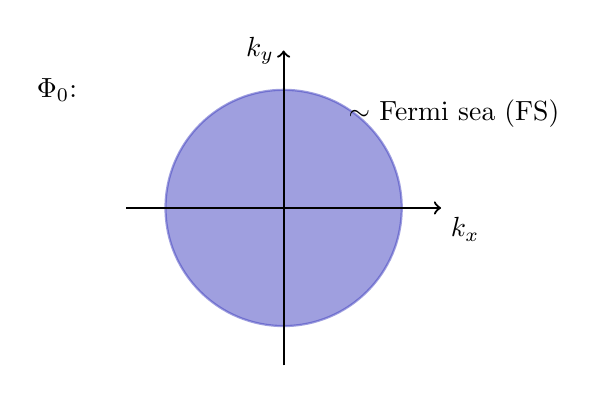
\begin{tikzpicture}[scale = 1]
	
	\coordinate (a) at (2, 2);
	\draw[thick,fill, blue!50!gray,  opacity =0.5] (a) circle (1.5);
	
	\draw[thick, ->] (0,2) to (4,2);
	\draw[thick, ->] (2,0) to (2,4);
	
	\node[anchor = north west] at (4, 2) {$k_x$};	
	
	\node[anchor = east] at (2, 4) {$k_y$};
	
	\node[anchor = east] at (-0.5, 3.5) {$\ket{\Phi_0}$:};
	\node[anchor = west] at (2.7, 3.2) {$\sim$ Fermi sea (FS)};
\end{tikzpicture}
%	\caption{The Fermi sea of $\ket{\Phi_0}$}
	\end{subfigure}	
	\begin{subfigure}{\linewidth}
	\centering
	\begin{tikzpicture}[scale=0.8]
	\begin{axis}[
	ticks=none,
	legend style={at={(1,0.4)}},
	ytick = {1},
	ytick style={draw=none},
	yticklabels = {},
	xtick = {1},
%	xticklabels ={$-\pi$,$\pi$},
	xtick style={draw=none},
	xlabel = \large $k$,
	ylabel = \large $\varepsilon_k$,
	axis lines = center,
	ymin = 0,
	ymax = 1.5,
	xmax = 2,
	xmin = -2,
	%x label style={at={(axis description cs:1,0.1)}, anchor = west},
	%y label style={at={(axis description cs:0.15,1)},rotate=-90,anchor=south},
	%xlabel = $x$,
	%sylabel = {$f(x)$},
	]
	
		
		\addplot[name path = A,domain = -1.57:1.57, samples = 200, very thin, black]{(1-cos(deg(x)))};
		\addplot[domain = -1.7:1.7, samples = 200, thick, red]{(1-cos(deg(x)))};
		\addplot[name path = B, domain = -1.57:1.57] {1+0*x};
		
		\addplot[fill,blue!50!gray, opacity=0.5] fill between[of = A and B];
		
		\draw[thick, black, dashed] (axis cs:-1.57,0) -- node[anchor= north east]{\large $-k_F$}  (axis cs:-1.570,1);
		\draw[thick, black, dashed] (axis cs:1.57,0) -- node[anchor= north west]{\large $k_F$}  (axis cs:1.570,1);
	\end{axis}
\end{tikzpicture}
	\caption{States are filled up to the energy $\ep_F$ at $k = k_F$ according to the Pauli-principle.}
	\end{subfigure}
\end{figure}

i) Consider first $t_2 >t_1$:

\begin{align*} 
&G_0(\lambda_1, t_1, \lambda_2, t_2) \\
 &=-i\theta(t_2-t_1)\ev{c_{k_2,\sigma_2}(t_2)c_{k_1\sigma_1}^\dagger(t_1)}{\Phi_0} \\
&=-i\theta(t_2-t_1)\ev{\e^{i\Ha_0t_2}c_{k_2\sigma_2}\e^{-i\Ha_0t_2}\e^{i\Ha_0t_1}c_{k_1\sigma_1}^\dagger\e^{-i\Ha_0t_1}}{\Phi_0} \\
&= -i\theta(t_2 - t_1) \ev{\e^{i(E_0 + \ep_{k_1}-\ep_{k_2})t_2}c_{k_2\sigma_2}\e^{-i(E_0 + \ep_{k_1})t_2}\e^{i(E_0 + \ep_{k_1})t_1}c_{k_1\sigma_1}^\dagger\e^{-E_0t_1}}{\Phi_0} \\
&= -i\theta(t_2-t_1)\e^{i(\ep_{k_1}-\ep_{k_1})t_2}\e^{-i\ep_{k_1}(t_2-t_1)}\underbrace{\ev{c_{k_2\sigma_2}c_{k_1\sigma_1}^\dagger}{\Phi_0}}_{\delta_{k_1k_2}\delta_{\sigma_1\sigma_2}\theta(\ep_{k_1} - \ep_{k_F})} \\
&= -i\theta(t_2-t_1)\e^{-i\ep_{k_1}(t_2-t_1)}\delta_{k_1k_2}\delta_{\sigma_1\sigma_2}\theta(\ep_{k_1} - \ep_{k_F})
\end{align*}


ii) $t_1>t_2$:

\begin{align*} 
&G_0(\lambda_1, t_1, \lambda_2, t_2) \\
&=-i\theta(t_1-t_2)(-1)\ev{c_{k_1\sigma_1}^\dagger(t_1)c_{k_2,\sigma_2}(t_2)}{\Phi_0} \\
&=i\theta(t_1-t_2)\ev{\e^{i\Ha_0t_1}c_{k_1\sigma_1}^\dagger\e^{-i\Ha_0t_1}\e^{i\Ha_0t_2}c_{k_2\sigma_2}\e^{-i\Ha_0t_2}}{\Phi_0} \\
&= i\theta(t_1-t_2) \ev{\e^{i(E_0 + \ep_{k_1}-\ep_{k_2})t_1}c_{k_1\sigma_1}^\dagger\e^{-i(E_0 - \ep_{k_2})t_1}\e^{i(E_0 - \ep_{k_2})t_2}c_{k_2\sigma_2}\e^{-E_0t_2}}{\Phi_0} \\
&= i\theta(t_1-t_2)\e^{i\ep_{k_1}t_1}\e^{-i\ep_{k_2}t_2}\delta_{k_1k_2}\delta_{\sigma_1\sigma_2}\theta(\ep_{k_F} - \ep_{k_1}) \\
&= i\theta(t_1-t_2)\delta_{k_1k_2}\delta_{\sigma_1\sigma_2}\theta(\ep_{k_F} - \ep_{k_1})\e^{-i\ep_{k_1}(t_2-t_1)}
\end{align*}

Therefore, 
\begin{align}
\label{eq:greens_time_domain}
\begin{split}
G_0(k_1\sigma_1, t_1;k_2\sigma_2, t_2) = &-i\theta(t_2-t_1)\theta(\ep_{k_1} - \ep_{k_F})\delta_{k_1k_2}\delta_{\sigma_1\sigma_2}\e^{-i\ep_{k_1}(t_2-t_1)}\\
&+ i \theta(t_1-t_2)\theta(\ep_{k_F} - \ep_{k_1})\delta_{k_1k_2}\delta_{\sigma_1\sigma_2}\e^{-i\ep_{k_1}(t_2-t_1)}
\end{split}
\end{align}
This is a rather unwieldy expression, so to simplify a bit, we set $t_2-t_1 = t$ and introduce Fourier-transformed $G_0$.

\begin{align*} 
G_0(k_1\sigma_1;k_2\sigma_2;\omega) &= \int_{-\infty}^\infty\dd{t}G_0(k_1\sigma_1;k_2\sigma_2 ; t)\e^{i\omega t} \\
&= -i\theta(\ep_{k_1} - \ep_{k_F})\delta_{k_1k_2}\delta_{\sigma_1\sigma_2}\int_{0}^\infty\dd{t}\e^{-i\ep_{k_1}t}\underbrace{\e^{-\delta t}}_{\delta = 0^+}\e^{i\omega t} \\
&+ i\theta(\ep_{k_F} - \ep_{k_1})\delta_{k_1k_2}\delta_{\sigma_1\sigma_2}\int_{-\infty}^0\dd{t}\e^{-i\ep_{k_1}t}\underbrace{\e^{\delta t}}_{\delta = 0^+}\e^{i\omega t} \\
&= -i\theta(\ep_{k_1} - \ep_{k_F})\delta_{k_1k_2}\delta_{\sigma_1\sigma_2}\int_{0}^\infty \dd{t}\e^{i(\omega -\ep_{k_1} + i\delta)t} \\
& + i\theta(\ep_{k_F} - \ep_{k_1})\delta_{k_1k_2}\delta_{\sigma_1\sigma_2}\int_{-\infty}^0\dd{t}\e^{i(\omega-\ep_{k_1}-i\delta)t} \\
&= \delta_{k_1k_2}\delta_{\sigma_1\sigma_2}\left( \frac{\theta(\ep_{k_1} - \ep_{k_F})}{\omega-\ep_{k_1} + i\delta} + \frac{\theta(\ep_{k_F}-\ep_{k_1})}{\omega - \ep_{k_1} - i\delta} \right)
\end{align*}
\begin{itemize}
	\item The first term in the Green's function involves excitations \underline{above} the Fermi-surface (particles), depicted in \cref{fig:fermi_sea_particle_excitation}.
	\begin{figure}
		\centering
		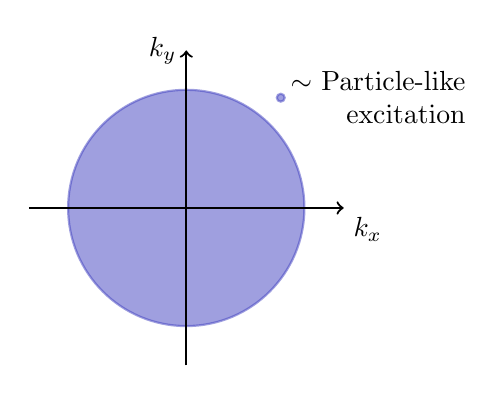
\begin{tikzpicture}[scale = 1]
	
	\coordinate (a) at (2, 2);
	\draw[thick,fill, blue!50!gray,  opacity =0.5] (a) circle (1.5);
	
	\draw[thick, ->] (0,2) to (4,2);
	\draw[thick, ->] (2,0) to (2,4);
	
	\node[anchor = north west] at (4, 2) {$k_x$};	
	
	\node[anchor = east] at (2, 4) {$k_y$};
	
	
	\draw[thick, fill, blue!50!gray, opacity=0.5] (3.2, 3.4) circle (0.05);
%	
%	\node[anchor = east] at (-0.5, 3.5) {$\ket{\Phi_0}$:};
	\node[anchor = west, align = right] at (3.2, 3.4) {$\sim$ Particle-like\\excitation};
\end{tikzpicture}
		\caption{Particle excitation above the Fermi-surface.}
		\label{fig:fermi_sea_particle_excitation}
	\end{figure}
	Particle created first, then destroyed later. Particle moves \underline{forward} in time. This is seen directly from the expression for $G_0$ in the time-domain, \cref{eq:greens_time_domain}, when $t_2 > t_1$ (particle created first at time $t_1$, then destroyed later at time $t_2$).
	\item The second term in the Green's function involves excitations \underline{below} the Fermi-surface (holes), depicted in \cref{fig:fermi_sea_hole_excitation}.
	\begin{figure}
		\centering
		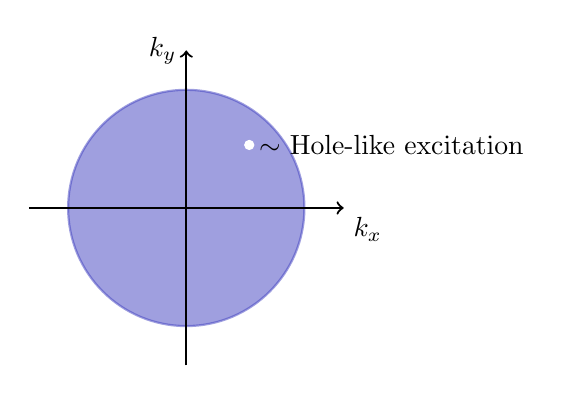
\begin{tikzpicture}[scale = 1]
	
	\coordinate (a) at (2, 2);
	\draw[thick,fill, blue!50!gray,  opacity =0.5] (a) circle (1.5);
	
	\draw[thick, ->] (0,2) to (4,2);
	\draw[thick, ->] (2,0) to (2,4);
	
	\node[anchor = north west] at (4, 2) {$k_x$};	
	
	\node[anchor = east] at (2, 4) {$k_y$};
	
	
	\coordinate (c) at (2.8, 2.8);
	\draw[thick, fill, white] (c) circle (0.05);
%	
%	\node[anchor = east] at (-0.5, 3.5) {$\ket{\Phi_0}$:};
	\node[anchor = west, align = right] at (c) {$\sim$ Hole-like excitation};
\end{tikzpicture}
		\caption{Hole excitation below the Fermi-surface.}
		\label{fig:fermi_sea_hole_excitation}
	\end{figure}
	Particle destroyed first, then created later. Particle moves \underline{backwards} in time. This is again seen directly in \cref{eq:greens_time_domain}.
	\item The part of $G_0$ that moves a particle \underline{forward in time} is often referred to as a \underline{retarded Green's function} $G_0^R$.
	\item The part of $G_0$ that moves a particle \underline{backwards in time} is often referred to as a \underline{advanced Green's function} $G_0^A$.
\end{itemize}


\begin{align} 
G_0^R(k_1, \sigma_1;k_2, \sigma_2;\omega) &= \frac{\theta(\ep_{k_1}-\ep_F)}{\omega_-\ep_{k_1} + i\delta}\delta_{k_1k_2}\delta_{\sigma_1\sigma_2}\\
G_0^A(k_1, \sigma_1;k_2, \sigma_2;\omega) &= \frac{\theta(\ep_F - \ep_{k_1})}{\omega_-\ep_{k_1} - i\delta}\delta_{k_1k_2}\delta_{\sigma_1\sigma_2}
\end{align}
With the understanding that in $G_0$, we must have $k_1 = k_2$; $\sigma_1 = \sigma_2$ and $\ep_{k_1}>\ep_F$ in $G^R$, $\ep_{k_!}<\ep_F$ in $G^A$, we may write
\begin{align} 
G_0^R(k, \omega) &= \frac{1}{\omega -\ep_k + i\delta} \\
G_0^A(k, \omega) &= \frac{1}{\omega -\ep_k -i\delta},
\end{align}
which is summarized by
\begin{align} 
G_0(k, \omega) &= \frac{1}{\omega-\ep_k + i\delta_k},
\end{align}
where $\delta_k = \delta\sign(\ep_k - \ep_F)$.
\begin{tcolorbox}
	Note that the single-particle excitation energies appear as simple poles in the Green's function!
\end{tcolorbox}
To aget a bit more perspective on things, consider $G_0^R (k,\omega)$ a bit further. $G_{0,R}^{-1} = \omega-\ep_k+i\delta$
Imagine that we now introduce $V \ne 0$. What will happen is that the excitation spectrum $\ep_k$ will change, due to the perturbation $G_{0R}^{-1} \rightarrow G_R^{-1}(k,\omega)$.
\begin{equation} 
G_R^{-1}(k,\omega) = \omega -\ep_k -\Sigma(k,\omega),
\end{equation}
$\Sigma(k,\omega) = \Sigma_{\text{Re}}(k,\omega) + i\Sigma_{\text{Im}}(k,\omega)$.
\begin{align*} 
\Sigma_{\text{Re}}: && \text{Real part of } \Sigma \\
\Sigma_{\text{Im}}: && \text{Imaginary part of } \Sigma
\end{align*}
Physicall interpretation og $G_R$: Create a particle in $(k,\sigma)$ at $t=0$. What is the probability amplitude of finding the particle in the same state at $t>0$? \underline{Answer: $G_R$}. $\Sigma(k,\omega)$ is the single particle self-energy.
Note: $G_R^{-1} = G_{0R}^{-1} - \Sigma$
\begin{align*} 
G_R &= \frac{1}{G_{0R}^{-1} - \Sigma} =\frac{G_{0R}}{1-G_{0R}\Sigma} \\
&= G_{0R} + G_{0R}\Sigma G_{0R} + G_{0R}\Sigma G_{0R} \Sigma G_{0R} + \dots
\end{align*}
We can generate a perturbation expansion for $G_R$ by a much simpler perturbation expansion for $\Sigma$!
Define the spectral weight $A_R(k,\omega)$
\begin{equation} 
\label{eq:spectral_function}
A_R(k,\omega) = -\frac{1}{\pi}\Im{G_R(k,\omega)}
\end{equation}
This is the quantity one measures in ARPES 
\begin{equation} 
A_R(k,\omega) = -\frac{1}{\pi}\frac{\Sigma_{\text{Im}}}{(\omega -\ep_k -\Sigma_{\text{Re}})^2-\Sigma_{\text{Im}}^2}
\end{equation}
In the non-interacting case:
$\Sigma_{\text{Im}} = 0, \Sigma_{\text{Im}} = -\delta; \delta = 0^+$
\begin{equation} 
A_{0R}(k, \omega) = -\frac{1}{\pi}\frac{-\delta}{(\omega-\ep_k)^2 + \delta^2} = \delta(\omega -\ep_k),
\end{equation}
which is a Dirac $\delta$-function, shown in \cref{fig:dirac_delta}. Send in photons of different energies and momenta to map out $\ep_k$. 
\begin{figure}
	\begin{subfigure}{0.5\linewidth}
	\centering
	\begin{tikzpicture}[scale=0.8]
	\begin{axis}[
%	ticks=none,
	legend style={at={(1,0.4)}},
	ytick = {1},
	ytick style={draw=none},
	yticklabels = {},
	xtick = {1},
	xticklabels ={\Large $\ep_k$},
%	xtick style={draw=none},
	xlabel = \Large $\omega$,
	ylabel = \Large $A_{0R}$,
	axis lines = center,
%	ymin = 0,
	ymax = 1.5,
%	xmax = 2,
%	xmin = -2,
	x label style={at={(axis description cs:1,0.1)}, anchor = west},
	y label style={at={(axis description cs:0,1)},rotate=0,anchor=west},
	%xlabel = $x$,
	%sylabel = {$f(x)$},
	]
	
		
		\addplot[name path = A,domain = 0:2, samples = 200, blue!50!gray, opacity=0.5, very thick]{0.001/((x-1)^2 + 0.001^2)};
%		\addplot[domain = -1.7:1.7, samples = 200, thick, red]{(1-cos(deg(x)))};
%		\addplot[name path = B, domain = -1.57:1.57] {1+0*x};
		
		\node[anchor= west, align=center] at (axis cs:1,1) {\Large{ $\sim \delta-$function}\\\Large {peak}};
		
%		\draw[thick, black, dashed] (axis cs:-1.57,0) -- node[anchor= north east]{\large $-k_F$}  (axis cs:-1.570,1);
%		\draw[thick, black, dashed] (axis cs:1.57,0) -- node[anchor= north west]{\large $k_F$}  (axis cs:1.570,1);
	\end{axis}
\end{tikzpicture}
	\caption{Non-interacting system.}
	\label{fig:dirac_delta}
	\end{subfigure}
	\begin{subfigure}{0.5\linewidth}
	\centering
	\begin{tikzpicture}[scale=0.8]
	\begin{axis}[
%	ticks=none,
	legend style={at={(1,0.4)}},
	ytick = {1},
	ytick style={draw=none},
	yticklabels = {},
	xtick = {1},
	xticklabels ={\Large $\ep_k + \Sigma_{\text{Re}}$},
%	xtick style={draw=none},
	xlabel = \Large $\omega$,
	ylabel = \Large $A_{R}$,
	axis lines = center,
%	ymin = 0,
	ymax = 9,
%	xmax = 2,
%	xmin = -2,
	x label style={at={(axis description cs:1,0.1)}, anchor = west},
	y label style={at={(axis description cs:0,1)},rotate=0,anchor=west},
	%xlabel = $x$,
	%sylabel = {$f(x)$},
	]
	
		
		\addplot[name path = A,domain = 0:2, samples = 200, black]{0.15/((x-1)^2 + 0.15^2)};
%		\addplot[domain = -1.7:1.7, samples = 200, thick, red]{(1-cos(deg(x)))};
%		\addplot[name path = B, domain = -1.57:1.57] {1+0*x};
		
		\node[anchor= west, align=center] at (axis cs:1.15,3.4) {\Large{$\sim \Sigma_{\text{Im}}$}};
		
		\draw[black, dashed] (axis cs:1,0) --  (axis cs:1,9);
		\draw[very thick, black] (axis cs:1,3.4) --  (axis cs:1.15,3.4);
%		\draw[thick, black, dashed] (axis cs:1.57,0) -- node[anchor= north west]{\large $k_F$}  (axis cs:1.570,1);
	\end{axis}
\end{tikzpicture}
	\caption{Interacting system.}
	\label{fig:lorentzian}
	\end{subfigure}
	\caption{Spectral weights for both interacting and non-interacting system.}
\end{figure}
For $V\ne 0:$ Peak position is shifted, narrow peak is broadened, as shown in \cref{fig:lorentzian}.
From maximum in peak: $\ep_k + \Sigma_{\text{Re}} = \tilde{\ep}_k$. From width of peak: $\Sigma_{\text{Im}}$.
$\Sigma = \Sigma_{\text{Re}} + i\Sigma_{\text{Im}}$. $\Sigma_{\text{Re}}$ and $\Sigma_{\text{Im}}$ are related via the Kramers-Kronig relations
\begin{equation} 
\Sigma_R(k,\omega) = \frac{1}{\pi}\mathcal{P}\int_{-\infty}^\infty\dd{\omega'}\frac{\Sigma_{\text{Im}}(k,\omega')}{\omega'-\omega}.
\end{equation}
Therefore, from width of peak $\rightarrow \Sigma_{\text{Im}}$. From Kramers-Kronig: $\Sigma_{\text{Re}}$. This allows an ARPES experiment to uniquely determine both $\Sigma_{\text{Im}}$ and $\Sigma_{\text{Re}}$ from one measurement, and thus to back out the many-body effect in  $\tilde{\ep}_k$, the quasiparticle excitation spectrum. Note: For Kramers-Kronig to hold, $\Sigma(k,\omega)$ need to be analytic in the upper half-plane when $\omega$ is viewed as a complex variable. Moreover, $\Sigma$ must fall off faster than $\frac{1}{|\omega|}$ when $|\omega| \rightarrow \infty.$ For the perturbations we will consider, this will be the case. 
\begin{tcolorbox}
	Our goal will therefore be to compute $\Sigma$ in many-body perturbation theory.
\end{tcolorbox}
Before we go into this, it will be turn out to be necessary to also consider bosonic Green's functions, and we start with the non-interacting case
\subsubsection{Bosons} % Lecture notes week 7

\begin{align*} 
D(q, t-t') &= -i\ev{\tilde{T}[\hat{A}_q(t)\hat{A}_q^\dagger(t')]}{\Psi(0)} \\
&= -i\frac{\ev{\tilde{T}[\hat{A}_q(t)\hat{A}_q^\dagger(t')S(\infty, -\infty)]}{\Phi_0}}{\ev{S(\infty, -\infty)}{\Phi_0}}.
\end{align*}
$\ket{\Phi_0}$: Unperturbed ground state of bosonic system. 
\begin{equation} 
\label{eq:non_int_greens_boson}
D_0(q, t-t') = -i\ev{\tilde{T}[\hat{A}_q(t)\hat{A}_q^\dagger(t')]}{\Phi_0}.
\end{equation}
Retarded boson-propagator: $t'<t$. Advanced boson-propagator: $t'>t$. At $T = 0$, the lowest energy state is occupied by all bosons (material particles), or there are no bosons present at all (phonons, magnons).
Let us focus in the following focus on \underline{phonons}.
\begin{align*} 
A_q &= a_q + a_{-q}^\dagger \\
A_q(t) &= \e^{i\Ha_0 t}A_q\e^{-i\Ha_0t} \\
\Ha_0 &= \sum_{q, \lambda }\omega_{q, \lambda}a_{q,\lambda}^\dagger a_{q,\lambda} \\
\Ha_0\ket{\Phi_0} &= 0 = E_0\ket{\Phi_0}, E_0 = 0
\end{align*}
$t'=0$, since $D_0$ will only be a function of $t-t'$ anyway. This is no loss of generality.

\textbf{$t>0$}:
\begin{align} 
\begin{split} 
D_0(q, \lambda, t) &= -i\theta(t)\ev{\e^{i\Ha_0 t}A_{q\lambda}\e^{-i\Ha_0t}A_{q\lambda}^\dagger}{\Phi_0} \\
&= -i\theta(t)\ev{A_{q\lambda}A_{q\lambda}^\dagger}{\Phi_0}\e^{-i\omega_{q,\lambda}t}\\
&= -i\theta(t)\e^{-i\omega_{q, \lambda}t}
\end{split}
\end{align}

\textbf{$t<0$}:
\begin{align} 
\begin{split} 
D_0(q, \lambda, t) &= -i\theta(-t)\ev{A_{q\lambda}^\dagger\e^{i\Ha_0 t}A_{q\lambda}\e^{-i\Ha_0t}}{\Phi_0} \\
&= -i\theta(-t)\ev{A_{q\lambda}^\dagger A_{q\lambda}}{\Phi_0}\e^{i\omega_{q,\lambda}t}\\
&= -i\theta(-t)\e^{i\omega_{q, \lambda}t}.
\end{split}
\end{align}

In total we have
\begin{equation} 
D_0(q, \lambda, t) = -\theta(t)\e^{-i\omega_{q, \lambda}t} -i\theta(-i)\e^{i\omega_{q,\lambda}t}.
\end{equation}
Note the sign change in the phase factor due to $A_q = a_q+ a_{-q}^\dagger$.
As for the fermionic case, let us Fourier-transform this, using shorthand notation $q = (q, \lambda)$.

\begin{align} 
\begin{split} 
D_0(q, \omega) &= \int_{-\infty}^\infty\dd{t}\e^{i\omega t}D_0(q, t) \\
&= -i\int_{0}^{\infty}\dd{t}\e^{i(\omega-\omega_{q} + i\delta)t} -i \int_{-\infty}^{0}\dd{t}\e^{i(\omega + \omega_{q} -i\delta)t} \\
&= \frac{1}{\omega -\omega_q + i\delta} - \frac{1}{\omega + \omega_q -i\delta} \\
&= \frac{2\omega_q}{\omega^2-\omega_q^2 + i\eta}.
\end{split}
\end{align}
Here, it does not make sense to consider retarded and advanced parts as for the fermions, since $A_q = a_q + a_{-q}^\dagger$
\begin{equation} 
D_0^{-1} = \frac{\omega^2 - \omega_q^2}{2\omega_q} + i\eta
\end{equation}
Imagine now that we turn on interactions (between phonons and electrons, for example)

\begin{tcolorbox}
\begin{equation} 
D_0^{-1} \rightarrow D^{-1} = D_{0}^{-1} - \Pi
\end{equation}
\end{tcolorbox}
$\Pi:$ Phonon self-energy.
\begin{align*} 
D &= \frac{1}{D_0^{-1} - \Pi} = \frac{D_0}{1-\Pi D_0} \\
&= D_0  + D_0\Pi D_0 + D_0 \Pi D_0\Pi D_0 + \dots
\end{align*}
Again; Perturbation series for $D$ by much simpler perturbation series for $\Pi$!

The equations
\begin{align} 
G_R^{-1} &= G_{0R}^{-1} - \Sigma \\
D^{-1} &= D_{0}^{-1} - \Pi
\end{align}
are usually referred to as the \textbf{Dyson's equations} for single-particle Green's functions. The physicall interpretations for $G$ and $D$ are the same (but of course applies to two different sorts of particles.)
In the following, we will consider electron- phonon coupling as a perturbation. The phonons will lead to a $\Sigma$, and the electrons in turn will lead to a $\Pi$.

\subsection[Single particle Green's function]{Perturbation theory for the single-particle Green's function}
Denote this Green's function by $G(\lambda, t-t')$. We have previously argued that in the presence of interactions it may be expressed as follows
\begin{equation} 
G^{-1} = G_0^{-1} - \Sigma
\end{equation}
where $G_0$ is the single-particle Green's function in the non-interacting case, and $\Sigma$ is the self-energy. Thus, our perturbation theory for $G$ may be found by a perturbation expansion for $\Sigma$, which we may hope is easier to compute than a perturbation theory for $G$ directly. The basic mathematical expression for $G$ is, starting in the Heisenberg-picture
\begin{equation} 
G(\lambda, t-t') = -i\ev{\tilde{T}[\hat{c}_\lambda(t)\hat{c}_\lambda^\dagger(t')]}{\psi(0)}
\end{equation}
where $\ket{\psi(0)}$ are exact eigenstates and 
\begin{equation} 
\hat{c}_\lambda(t) = \e^{i\Ha t}c_\lambda\e^{-i\Ha t}.
\end{equation}
Translated into interaction picture, we have
\begin{equation} 
G(\lambda, t-t') = -i\frac{\ev{\tilde{T}[{c}_{\lambda}(t){c}_{\lambda}^\dagger(t')S(\infty, -\infty)]}{\Phi_0}}{\ev{S(\infty, -\infty)}{\Phi_0}},
\end{equation}
where $S$ is the $S$-matrix,
\begin{equation} 
c_\lambda(t) = \e^{i\Ha_0 t}c_\lambda\e^{-i\Ha_0 t},
\end{equation}
and $\ket{\Phi_0}$  is the eigenstate of $\Ha_0$, assumed to be known to us. 
Both of these expressions are formally exact, while the second one allows a systematic expansion in powers of $V(t)$, where
\begin{equation} 
V(t) = \e^{i\Ha_0 t}V\e^{-i\Ha_0 t}
\end{equation}
and $\Ha = \Ha_0 + V$.
For $S(\infty, -\infty)$, we have (remember \cref{eq:s_matrix})
\begin{equation} 
S(t, t') =  \sum_{n=0}^{\infty}\frac{(-i)^n}{n!}\int_{t'}^{t}\dd{t_1}\cdots\int_{t'}^{t}\dd{t_n}\tilde{T}[V(t_1)\cdots V(t_n)]
\end{equation}
where the $n=0$-term is 1. 
In these notes, we will focus on $V$ taken to be the electron-phonon coupling. Another obvious choice would be the Coulomb-interaction. 
\begin{equation}
\label{eq:el_ph}
V =\sum_{k,q, \sigma, \lambda}g_{q\lambda}A_{q\lambda} c_{k+q,\sigma}^\dagger c_{k,\sigma},
\end{equation}
$A_{q\lambda} = a_{-q,\lambda}^\dagger + a_{q\lambda}$.

\begin{align*} 
V(t) &= \e^{i\Ha_0 t}V\e^{-i\Ha_0 t} \\
&=  \sum_{k,q, \sigma, \lambda}g_{q\lambda}\e^{i\Ha_0 t}A_{q\lambda} c_{k+q,\sigma}^\dagger c_{k,\sigma}\e^{-i\Ha_0 t} \\
&= \sum_{k,q, \sigma, \lambda}g_{q\lambda}\left(\vphantom{c_{k+q,\sigma}^\dagger}\e^{i\Ha_0 t}A_{q\lambda}\e^{-i\Ha_0 t}\right)\left( \e^{i\Ha_0 t}c_{k+q,\sigma}^\dagger\e^{-i\Ha_0 t}\right)\left( \vphantom{c_{k+q,\sigma}^\dagger} \e^{i\Ha_0 t}c_{k,\sigma}\e^{-i\Ha_0 t}\right)
\end{align*}
\begin{tcolorbox}
	\begin{equation}
	\label{eq:el_ph_time}
		V(t) = \sum_{k, q, \sigma, \lambda}g_{q\lambda}A_{q\lambda}(t) c_{k+q,\sigma}^\dagger(t) c_{k,\sigma}(t)
	\end{equation}
\end{tcolorbox}
Compare $V(t)$ in \cref{eq:el_ph_time} to $V$ in \cref{eq:el_ph}. All time-dependence of operators is in the interaction picture. $V(t)$ is the perturbation we will use in $ S(\infty, -\infty) $ and thus $G(\lambda, t-t')$. The expectation values we will have to compute will then consist of a product of $ (c^\dagger, c)$-operators multiplied by a product of $ A$-operators. 
Each $ V $ will give a factor $ Ac^\dagger c $. Thus, $n$ factors of $V$ will give
\begin{equation} 
\left.\begin{array}{cc}
n+1 & c^\dagger \text{-factors} \\
n+1 & c \text{-factors} \\
n & A\text{ -factors}
\end{array}\right\} \text{ in } G
\end{equation}
The extra 1 in $n+1$ comes from $c_\lambda^\dagger(t'), c_\lambda(t)$  in the definition of $G$. Now, we factorize $\ket{\Phi_0}$ in a \textbf{boson-part} and a \textbf{fermion-part}. 
\begin{equation} 
\left.\begin{array}{cc}
\text{ Boson-part: } & \ket{\Phi_0}_B \\
\text{ Fermion-part: } & \ket{\Phi_0}_F
\end{array}\right\} \implies \ket{\Phi_0} = \ket{\Phi_0}_B \otimes \ket{\Phi_0}_F.
\end{equation}
\begin{align} 
\begin{split} 
G(\lambda, t-t') &= \frac{-i}{\ev{S(\infty, -\infty)}{\Phi_0}}\sum_{n=0}^{\infty}\frac{(-i)^n}{n!}\int_{-\infty}^{\infty}\dd{t_1}\dots  \int_{-\infty}^{\infty}\dd{t_n} \\
& \cdot \ev{\tilde{T}[c_\lambda(t)c_\lambda^\dagger(t')V(t_1)\dots V(t_n)]}{\Phi_0}.
\end{split}
\end{align}
$[\ \cdot\ ]$: A product of $n+1$ $ c^\dagger, c $-operators and $n$ $A(t_i)$-operators. The expectation value of the fermion-operators are taken in $\ket{\Phi_0}_F$, while the expectation value of the boson-operators are taken in $\ket{\Phi_0}_B$. The expectation value may thus be written
\begin{align*} 
&{}_B\ev{\tilde{T}[A_{q_1}(t_1)\dots A_{q_n}(t_n)]}{\Phi_0}_B\\
& \cdot {}_F\ev{\tilde{T}[c_\lambda(t)c_\lambda^\dagger(t') c_{k_1+q, \sigma_1}^\dagger(t_1) c_{k_1\sigma_1}(t_1)\dots c_{k_n+q, \sigma_n}^\dagger(t_n) c_{k_n\sigma_n}(t_n)]}{\Phi_0}_F
\end{align*}
\textbf{NB!} Be careful with the ordering of operators! We see that as $n$ increases, the number of operators rapidly becomes sizeable, particularly in the fermionic part. One thing we immediately note, is that for these expectation values to be non-zero, we must have an even number of $A$-operators. Thus, for the electron-phonon coupling, only even powers of $ V $ contribute to the perturbation-series for $G$. (This is not the case if $V$ were taken to be the Coulomb-interaction, which contains $c^\dagger c^\dagger c c$ and no boson-operators.)
The lowest order term we need to consider, is therefore $n=2$, which contains 2 $A$-operators and 6 fermion-operators. For $n=2$, the boson-part is easy. Recall that 
\begin{align*} 
D_0(q, t) = -i {}_B&\ev{\tilde{T}[A_q(t)A_q(0)]}{\Phi_0}_B \\
\implies& \\
{}_B&\ev{\tilde{T}[A_q(t_1)A_q(t_2)]}{\Phi_0}_0 = iD_0(q, t_1-t_2),
\end{align*}
the free phonon Green's function we already computed. 
Next, we need to deal with the expectation value of a string of a fairly large number of fermion-operators (6 of them for $n=2$. 3$c^\dagger $ and $3 c$).
To do this, we use a theorem which we give here without proof. 
\begin{tcolorbox}[title= Wicks theorem]

To compute the $\ket{\Phi_0}_F$-expectation value of a product of equally many $c^\dagger$ and $c$-operators, we pair in all possible ways and compute the expectation value as products of expectation values of one $c^\dagger$ and one $c$. 
\end{tcolorbox}
\textbf{NB!} When pairing up non-adjacent $c^\dagger $ and $c$, use anti-commutation relations to bring them side by side to compute an expectation value.
Suppose we have a product of $N$ creation operators and $N$ destruction operators (bosonic of fermionic). The number of terms we then get by applying Wick's theorem is $N!$ Thus for $n=2$ with 3 $c^\dagger$ and 3 $c$, the number of terms is $3! =6$. 
To fourth order, the number of bosonic terms will be $6\cdot2! = 12 $ (since when expanding $A_q = a_{-q}^\dagger + a_q$ to fourth order there are 6 terms with 2 $a^\dagger$ and 2 $a$, and Wick's theorem applied to each of them gives another factor 2. The number of fermionic terms is given by $N= n+1 = 5 \rightarrow 5! =120. $ Altogether $12\cdot 120 = 1440$ terms. This rapidly gets out of hand, if we don't think a little and organize the calculations in a smart way. 
Recall the definitions of the non-interacting Green's functions of \cref{eq:non_int_greens_boson,eq:non_int_greens_fermion};
\begin{align} 
D_0(q_1, t_1-t_2)\delta_{q_1, q_2} &= -i\ev{\tilde{T}[A_{q_1}(t)A_{q_2}^\dagger(t')]}{\Phi_0}_B\\[2ex]
G_0(k_1, t_1-t_2)\delta_{k_1k_2}\delta_{\sigma_1\sigma_2} &= -i\ev{\tilde{T}[c_{k_1\sigma_1}^\dagger(t_1)c_{k_2\sigma_2}(t_2)]}{\Phi_0}_F
\end{align}
We will give these the following pictorial representation:
\begin{equation}
D_0(q_1, t_1-t_2): \quad 
\begin{tikzpicture}
\begin{feynman}
\vertex [small, dot](a) {};
\vertex [small, dot, right = 2cm of a] (b) {};
\diagram*{(a) [dot] --[boson, edge label=$q_1$] (b) [dot]};
\node[anchor = east] at (a) {$t_1$};
\node[anchor = west] at (b) {$t_2$};	
\end{feynman}
\end{tikzpicture}
\end{equation}
\begin{equation} 
G_0(k_1, t_1-t_2): \quad 
\begin{tikzpicture}
\begin{feynman}
\vertex [small, dot](a) {};
\vertex [small, dot, right = 2cm of a] (b) {};
\diagram*{(a) [dot] --[fermion] (b) [dot]};
\node[anchor = east] at (a) {$t_1$};
\node[anchor = west] at (b) {$t_2$};	
\end{feynman}
\end{tikzpicture}
\end{equation}
These will turn out to be very helpful later on. 

\underline{Start with $\ev{S(\infty, -\infty)}{\Phi_0}$}:
\begin{align*} 
&\ev{S(\infty, -\infty)}{\Phi_0} \\
&= 1 + \frac{(-i)^2}{2!}\int_{-\infty}^\infty\dd{t_1}\int_{-\infty}^\infty\dd{t_2}\ev{\tilde{T}[V(t_1)V(t_2)]}{\Phi_0} + \mathcal{O}(V^4)
\end{align*}
Consider now in detail the second term

\begin{align*} 
\frac{(-i)^2}{2!}&\int_{-\infty}^\infty\dd{t_1}\int_{-\infty}^\infty\dd{t_2}\sum_{k_1, q_1, \sigma_1}\sum_{k_2, q_2, \sigma_2}g_{g_1}g_{q_2}\\
&\cdot{}_B\ev{\tilde{T}[A_{q_1}(t_1)\underbrace{A_{q_2}(t_2)}_{=A_{-q_2}^\dagger(t_2)}]}{\Phi_0}_B \\
&\cdot {}_F\ev{\tilde{T}[c_{k_1+q_1, \sigma_1}^\dagger(t_1) c_{k_1\sigma_1}(t_1) c_{k_2+q_2, \sigma_2}^\dagger(t_2) c_{k_2\sigma_2}(t_2)]}{\Phi_0}_F
\end{align*}
The bosonic expectation value $= iD_0(q_1, t_1-t_2)\delta_{q_1, -q_2}$. In the fermionic part, use Wick's theorem. There are 2 ways to pair the $c^\dagger$'s with the $c$'s.
\begin{enumerate}[i)]
	\item \begin{equation}
		\wick{\c1 c_{k_1+q_1, \sigma_1}^\dagger \c1 c_{k_1\sigma_1} \c2 c_{k_2+q_2, \sigma_2}^\dagger \c2 c_{k_2\sigma_2}}
	\end{equation}
	\item \begin{equation}
	\wick{\c1 c_{k_1+q_1, \sigma_1}^\dagger \c2 c_{k_1\sigma_1} \c2 c_{k_2+q_2, \sigma_2}^\dagger \c1 c_{k_2\sigma_2}}
	\end{equation}
\end{enumerate}
with the corresponding equations
\begin{enumerate}[i)]
	\item \begin{align}
	\begin{split} 
	(+i)&G_0(k_1+q_1, t_1-t_1)\delta_{k_1+q_1,k_1}\cdot(-1)\\
	\cdot(+i)&G_0(k_2+q_2, t_2-t_2)\delta_{k_2+q_2,k_2}\cdot(-1)
	\end{split}	
	\end{align}
	
	\item 
	\begin{align}
	\begin{split} 
	(+i)&G_0(k_1+q_1, t_2-t_1)\delta_{k_1+q_1,k_2}\delta_{\sigma_1\sigma_2}\cdot(-1)^3\\
	\cdot(+i)&G_0(k_2+q_2, t_1-t_2)\delta_{k_2+q_2,k_1}\delta_{\sigma_1\sigma_2}\cdot(-1)
	\end{split}	
	\end{align}
\end{enumerate}
In i), note that the $\delta$-functions in $k$ from the fermionic part forces $q_1 =0, q_2 = 0$.
Multiplying all the factors of i):
\begin{center}
\begin{tikzpicture}
	\begin{feynman}[large]
	\vertex [small, dot] (a) {};
	\vertex [small, dot, right = 3cm of a] (b) {};
	\diagram*{
	a --[anti fermion,loop, min distance=3cm] a -- [boson, edge label'=$q_1$] (b) -- [anti fermion,loop, min distance=3cm] b,	
};
	\node[anchor = east] at ($(a)+(-0.1,0)$) {$g_{-q_1}$};
	\node[anchor = west] at ($(b)+(0.1,0)$)  {$g_{q_1}$};
	\node[anchor = north] at ($(a)+(-0.1,-0.1)$) {$t_1$};
	\node[anchor = north] at ($(b)+(0.1,-0.1)$)  {$t_2$};	
	\end{feynman}
\end{tikzpicture}
\end{center}
But $q_1=q_2 = 0$. Since $g_q =0$ when $q=0$, this contribution to $S$ vanishes.
Consider next ii), which has the following representation:
\begin{center}
	\begin{tikzpicture}
		\begin{feynman}[large]
		\vertex [small, dot] (a) {};
		\vertex [small, dot, right = 3cm of a] (b) {};
		\diagram*{a -- [quarter right, fermion, edge label'={$k_1 + q_1, \sigma_1$}] (b) -- [quarter right, fermion, edge label'={$k_1, \sigma_1$}] a -- [boson, edge label'=$q_1$] (b),};
		
		\node[anchor = east] at ($(a)+(-0.1,0)$) {$g_{-q_1}$};
		\node[anchor = west] at ($(b)+(0.1,0)$)  {$g_{q_1}$};
		\node[anchor = north] at ($(a)+(-0.1,-0.1)$) {$t_1$};
		\node[anchor = north] at ($(b)+(0.1,-0.1)$)  {$t_2$};	
		\end{feynman}
	\end{tikzpicture}
\end{center}
Here, $q_1$ is not restricted to zero, so this contribution is nonzero. We must integrate over $t_1, t_2$, sum over $k_1, q_1, \sigma_1$.
Note $g_{q_1}g_{-q_1} = g_{q_1}g_{q_1}^* = |g_{q_1}|^2$. So to $\mathcal{O}(V^2)$, we have 
\begin{equation} 
\ev{S}{\Phi_0} = 1 +
\begin{gathered}
\feynmandiagram[scale = 2, transform shape][large, horizontal = a to b]{a -- [quarter right, fermion] b -- [quarter right, fermion] a -- [boson] b,};
\end{gathered} 
\end{equation}
The first term is simply the normalization of $\ket{\Phi_0}$. The second contribution is a quantum fluctuation effect in $\ket{\Phi_0}$ due to the presence of phonons. These phonons ``disturb'' the inert state $\ket{\Phi_0}$. This is often called a vacuum-fluctuation. and is a quantum fluctuation effect, which is present even when the system is left all by itself. Note that this contribution enters into the denominator of the Green's function we are in the process of computing. 

Consider next the numerator in $G$. The only difference between the numerator and $\ev{S(\infty, -\infty)}{\Phi_0}$ is the extra $c_{ k\sigma}(t)\cd_{ k\sigma}(t')$. The bosonic part is therefore\ exactly as in  $\ev{S(\infty, -\infty)}{\Phi_0}$, but the fermionic part now have 3 $\cd$'s and 3 $c$'s, instead of 2 $\cd$'s and 2 $c$'s.
We therefore consider only this fermionic expectation value, remembering that the result must be multiplied with\begin{equation} 
iD_0(q_1, t_1-t_2)\delta_{q_1, -q_2}g_{q_1}g_{q_2}. 
\end{equation}
The fermionic expectation value is
\begin{equation} 
{}_F\ev{\tilde{T}[c_{k\sigma}(t)c_{k\sigma}^\dagger(t') c_{k_1+q_1, \sigma_1}^\dagger(t_1) c_{k_1\sigma_1}(t_1) c_{k_2+q_2, \sigma_2}^\dagger(t_2) c_{k_2\sigma_2}(t_2)]}{\Phi_0}_F.
\end{equation}
Using Wicks theorem, the terms are
% c\cd \cd_1 c_1 \cd_2 c_2
\begin{enumerate}[1)]
	\item 
	\begin{equation} 
	\wick{\c c_{k\sigma} \c c_{k\sigma}^\dagger \c c_{k_1+q_1, \sigma_1}^\dagger \c c_{k_1\sigma_1} \c c_{k_2+q_2, \sigma_2}^\dagger \c c_{k_2\sigma_2}}
	\end{equation}
	$\implies \delta_{k_1 + q_1, k_1}\delta_{k_2 + q_2, k_2}\delta_{\sigma_1\sigma_2} \implies q_1=q_2 = 0 \implies \underline{1) = 0}.$
	\item
	\begin{equation} 
	\wick{\c1 c_{k\sigma} \c2 c_{k\sigma}^\dagger \c1 c_{k_1+q_1, \sigma_1}^\dagger \c2 c_{k_1\sigma_1} \c c_{k_2+q_2, \sigma_2}^\dagger \c c_{k_2\sigma_2}}
	\end{equation}
	$\implies \delta_{k, k_1+q_1}\delta_{\sigma, \sigma_1}\delta_{k, k_1}\delta_{k_2 + q_2, k_2} \implies q_2 = 0 \implies \underline{2) = 0}$.\footnote{I think there is an error in the notes here for both 2) and 3) in the delta-functions, but the conclusions of zero contribution remains.}
	\item 
	\begin{equation} 
	\wick{\c1 c_{k\sigma} \c2 c_{k\sigma}^\dagger \c c_{k_1+q_1, \sigma_1}^\dagger \c c_{k_1\sigma_1} \c1 c_{k_2+q_2, \sigma_2}^\dagger \c2 c_{k_2\sigma_2}}
	\end{equation}
	$\implies \delta_{k, k_2 +q_2}\delta_{\sigma, \sigma_2}\delta_{k, k_2}\delta_{k_1+q_1, k_1} \implies q_1 = 0 \implies \underline{3) = 0}$.
	\item
	\begin{equation} 
	\wick{\c c_{k\sigma} \c c_{k\sigma}^\dagger \c1 c_{k_1+q_1, \sigma_1}^\dagger \c2 c_{k_1\sigma_1} \c2 c_{k_2+q_2, \sigma_2}^\dagger \c1 c_{k_2\sigma_2}}
	\end{equation}
	\begin{align*} 
	=iG_0(k, t-t')&(-i)G_0(k_1+q_1, t_2-t_1)\delta_{k_1+q_1, k_2}\delta_{\sigma_1, \sigma_2} \\
	\cdot&(+i)G_0(k_1, t_1-t_2)\delta_{k_2+q_2, k_1}\delta_{\sigma_1, \sigma_2}
	\end{align*}
	Let us give a pictorial representation of this:
	\begin{center}
		\begin{tikzpicture}
		\begin{feynman}[large]
		\vertex [small, dot] (a) {};
		\vertex [small, dot, right = 3cm of a] (b) {};
		\vertex [small, dot, above = 1.5cm of a] (c) {};
		\vertex [small, dot, right = 3cm of c] (d) {};
		\diagram*{a -- [quarter right, fermion, edge label'={$k_1 + q_1, \sigma_1$}] (b) -- [quarter right, fermion, edge label'={$k_1, \sigma_1$}] a -- [boson, edge label'=$q_1$] (b),
		(c) -- [fermion, edge label = {$k, \sigma$}] (d)};
		
		\node[anchor = east] at ($(a)+(-0.1,0)$) {$g_{-q_1}$};
		\node[anchor = west] at ($(b)+(0.1,0)$)  {$g_{q_1}$};
		\node[anchor = north] at ($(a)+(-0.1,-0.1)$) {$t_1$};
		\node[anchor = north] at ($(b)+(0.1,-0.1)$)  {$t_2$};
		\node[anchor = north] at ($(c)+(-0.1,-0.1)$) {$t'$};
		\node[anchor = north] at ($(d)+(0.1,-0.1)$)  {$t$};
		\end{feynman}
		\end{tikzpicture}
	\end{center}
	This is a disconnected diagram. The interpretation of this is that the electron is disturbed by a quantum fluctuation in $\ket{\Phi_0}$, namely a vacuum-fluctuation. This vacuum-fluctuation is present even if we do not try to inject and extract an electron into the system. This is why the diagram comes out disconnected.
	\item 
	\begin{equation} 
	\wick{\c1 c_{k\sigma} \c2 c_{k\sigma}^\dagger \c1 c_{k_1+q_1, \sigma_1}^\dagger \c3 c_{k_1\sigma_1} \c3 c_{k_2+q_2, \sigma_2}^\dagger \c2 c_{k_2\sigma_2}}
	\end{equation}
	\begin{align*} 
	=(+i)&G_0(k, t-t_1)\delta_{k, k_1+q_1}\delta_{\sigma, \sigma_1}\\(+i)&G_0(k, t_2-t')\delta_{k,k_2}\delta_{\sigma, \sigma_2}\\
	(+i)&G_0(k_1, t_1-t_2)\delta_{k_1, k_2 + q_2}\delta_{\sigma_1, \sigma_2}(-1)^3
	\end{align*}
	We may give the following pictorial representation of this:
		\begin{center}
		\begin{tikzpicture}
		\begin{feynman}[large]
		\vertex [small, dot] (a) {};
		\vertex [small, dot, right = 3cm of a] (b) {};
		\vertex [small, dot, right = 3cm of b] (c) {};
		\vertex [small, dot, right = 3cm of c] (d) {};
		%		\vertex [small, dot, above = 1.5cm of a] (c) {};
		%		\vertex [small, dot, right = 3cm of c] (d) {};
		\diagram*{(a) -- [fermion, edge label={$k,\sigma$}] (b) -- [out=70,in=110, boson, edge label={$k-k_1$}] (c) -- [anti fermion, edge label={$k_1, \sigma$}] (b),
			(c) -- [fermion, edge label ={$k,\sigma$}] (d)
		};
		
		\node[anchor = east] at ($(b)+(-0.0,+0.2)$) {$g_{-q_1}$};
		\node[anchor = west] at ($(c)+(0.0,+0.2)$)  {$g_{q_1}$};
		\node[anchor = north] at ($(a)+(-0.1,-0.1)$) {$t'$};
		\node[anchor = north] at ($(b)+(0.1,-0.1)$)  {$t_2$};
		\node[anchor = north] at ($(c)+(-0.1,-0.1)$) {$t_1$};
		\node[anchor = north] at ($(d)+(-0.1,-0.1)$) {$t$};
		\end{feynman}
		\end{tikzpicture}
	\end{center}

	This is a connected diagram. The Green's function of the electron is disturbed by a quantum fluctuation, but in this case the quantum fluctuation is a direct result of injecting the electron into the system. 
	\item
	\begin{equation} 
	\wick{\c1 c_{k\sigma} \c2 c_{k\sigma}^\dagger \c3 c_{k_1+q_1, \sigma_1}^\dagger \c2 c_{k_1\sigma_1} \c1 c_{k_2+q_2, \sigma_2}^\dagger \c3 c_{k_2\sigma_2}}
	\end{equation}
	\begin{align*} 
	=(+i)&G_0(k, t-t_2)\delta_{k, k_2+q_2}\delta_{\sigma, \sigma_2}\\(-i)&G_0(k, t_1-t')\delta_{k,k_1+q_1}\delta_{\sigma, \sigma_1}\\
	(-i)&G_0(k_1 + q_1, t_2-t_1)\delta_{k_1 + q_1, k_2}\delta_{\sigma_1, \sigma_2}(-1)^4
	\end{align*}
	We may give the following pictorial description of this:
			\begin{center}
		\begin{tikzpicture}
		\begin{feynman}[large]
		\vertex [small, dot] (a) {};
		\vertex [small, dot, right = 3cm of a] (b) {};
		\vertex [small, dot, right = 3cm of b] (c) {};
		\vertex [small, dot, right = 3cm of c] (d) {};
		%		\vertex [small, dot, above = 1.5cm of a] (c) {};
		%		\vertex [small, dot, right = 3cm of c] (d) {};
		\diagram*{(a) -- [fermion, edge label={$k,\sigma$}] (b) -- [out=70,in=110, boson, edge label={$q_1$}] (c) -- [anti fermion, edge label={$k_1 + q_1, \sigma$}] (b),
			(c) -- [fermion, edge label ={$k,\sigma$}] (d)
		};
		
		\node[anchor = east] at ($(b)+(-0.0,+0.2)$) {$g_{-q_1}$};
		\node[anchor = west] at ($(c)+(0.0,+0.2)$)  {$g_{q_1}$};
		\node[anchor = north] at ($(a)+(-0.1,-0.1)$) {$t'$};
		\node[anchor = north] at ($(b)+(0.1,-0.1)$)  {$t_1$};
		\node[anchor = north] at ($(c)+(-0.1,-0.1)$) {$t_2$};
		\node[anchor = north] at ($(d)+(-0.1,-0.1)$) {$t$};
		\end{feynman}
		\end{tikzpicture}
	\end{center}
	Same as 5).
\end{enumerate}
Thus, we get to second order in $g$:
\begin{align*}
	G(k, t-t') &= -i\left\{
	\begin{gathered}
	\feynmandiagram[scale = 1, transform shape][horizontal = a to b]{a --[fermion] b};
	\end{gathered}
	+ 
	\begin{gathered}
	\begin{tikzpicture}
	\begin{feynman}[large]
	\vertex[small,dot] (a) {};
	\vertex [small, dot, right = of a] (b) {};
	\vertex [above = 0.5cm of a] (c) {};
	\vertex [above = 0.5cm of b] (d) {};
	\diagram*{a -- [quarter right, fermion] (b) -- [quarter right, fermion] a -- [boson] (b),
		(c) -- [fermion] (d)};
	\end{feynman}
	\end{tikzpicture}
	\end{gathered}\cdot(-i)^3(-1)
	\right.\\
	&\left. + 2(-i)^3(-1)\feynmandiagram[large][horizontal = a to d]{a--[fermion] b --[fermion] c -- [fermion] d, b--[half left, boson] c};
	+\dots \right\}\frac{1}{1 + \begin{gathered}
		\feynmandiagram[scale = 1, transform shape][large, horizontal = a to b]{a -- [quarter right, fermion] b -- [quarter right, fermion] a -- [boson] b,};
		\end{gathered}(+i)^2(-1)}
\end{align*}
\textbf{Schematically;} to second order in $g$:
\begin{align*}
	G = &\begin{gathered}
	\feynmandiagram[scale = 1, transform shape][horizontal = a to b]{a --[fermion] b};
	\end{gathered}\times \frac{\left(1 +
		\begin{gathered}
		\feynmandiagram[scale = 1, transform shape][large, horizontal = a to b]{a -- [quarter right, fermion] b -- [quarter right, fermion] a -- [boson] b,};
		\end{gathered} + \dots \right)}{1 +
		\begin{gathered}
		\feynmandiagram[scale = 1, transform shape][large, horizontal = a to b]{a -- [quarter right, fermion] b -- [quarter right, fermion] a -- [boson] b,};
		\end{gathered}} \\
	&+ \feynmandiagram[large][horizontal = a to d]{a--[fermion] b --[fermion] c -- [fermion] d, b--[half left, boson] c}; + \dots
\end{align*}
Disconnected diagrams cancel out. This will happen, order by order in $g$, to all orders. 
\begin{tcolorbox}[center, width =0.6\textwidth]
	$G$ is the sum of connected diagrams. 
\end{tcolorbox}
Thus, we are computing corrections to $G_0$ which come about as a direct result of quantum fluctuations that arise \textbf{because} we injected an electron into the system. The vacuum fluctuations cancel out. 
Imagine now that we compute corrections to  higher order in $g$, $g^4, g^6, \dots $ etc.
Schematically, we find 
\begin{align*}
G &=  \underset{g^0}{\begin{gathered}
\feynmandiagram[scale = 1, transform shape][horizontal = a to b]{a --[fermion] b};
\end{gathered}}
 + \underset{g^2}{\begin{gathered}
 \feynmandiagram[large][horizontal = a to d]{a--[fermion] b --[fermion] c -- [fermion] d, b--[half left, boson] c};
\end{gathered}} + \underset{g^4}{\begin{gathered}
\feynmandiagram[large][horizontal = a to f]{a--[fermion] b --[fermion] c -- [fermion] d --[fermion] e --[fermion] f, b--[half left, boson] c, d--[half left, boson] e};
\end{gathered}} \\
& + \underset{g^4}{\begin{gathered}
\begin{tikzpicture}
\begin{feynman}[scale=0.75, transform shape][large]
\vertex (a);
\vertex [right = of a] (b);
\vertex [right = of b] (c);
\vertex [right = of c] (d);
\vertex [above = 1cm of b] (t1) ;
\vertex [above = 1cm of c] (t2) ;
\diagram*{
	(a)--[fermion] (b) --[fermion](c) --[fermion](d),
	(b) --[boson] (t1),
	(c) --[boson] (t2),
	(t1)--[quarter left, fermion] (t2) -- [quarter left, fermion] (t1), 
	};
\end{feynman}
\end{tikzpicture}
\end{gathered}}
+ \underset{g^4}{\begin{gathered}
	\feynmandiagram[large][horizontal = a to f]{a--[fermion] b --[fermion] c -- [fermion] d --[fermion] e --[fermion] f, b--[quarter left, boson] e, c--[half right, boson] d};\end{gathered}} \\
&+ \underset{g^4}{\begin{gathered}
	\feynmandiagram[large][horizontal = a to f]{a--[fermion] b --[fermion] c -- [fermion] d --[fermion] e --[fermion] f, b--[quarter left, boson] d, c--[quarter right, boson] e};\end{gathered}} \\
&\left.
\begin{array}{ll}
&+\begin{gathered}\feynmandiagram[large][horizontal = a to h]{a--[fermion] b --[fermion] c -- [fermion] d --[fermion] e --[fermion] f--[fermion] g--[fermion] h, b--[quarter left, boson] d, c--[quarter right, boson] e, f--[quarter left, boson] g};\end{gathered} \\
&+\begin{gathered}\feynmandiagram[large][horizontal = a to h]{a--[fermion] b --[fermion] c -- [fermion] d --[fermion] e --[fermion] f--[fermion] g--[fermion] h, b--[quarter left, boson] c, d--[quarter left, boson] e, f--[quarter left, boson] g};\end{gathered} \\
&+ \begin{gathered}
\begin{tikzpicture}
\begin{feynman}[scale=0.75, transform shape][large]
\vertex (a);
\vertex [right = of a] (b);
\vertex [right = of b] (c);
\vertex [right = of c] (d);
\vertex [right = of d] (e);
\vertex [right = of e] (f);
\vertex [above = 1cm of b] (t1) ;
\vertex [above = 1cm of c] (t2) ;
\diagram*{
	(a)--[fermion] (b) --[fermion](c) --[fermion] (d) --[fermion] (e) --[fermion] (f),
	(b) --[boson] (t1),
	(c) --[boson] (t2),
	(t1)--[quarter left, fermion] (t2) -- [quarter left, fermion] (t1), 
	(d) --[quarter left, boson] (e)
};
\end{feynman}
\end{tikzpicture}
\end{gathered} \\
&+ \begin{gathered}
\begin{tikzpicture}
\begin{feynman}[scale=0.75, transform shape][large]
\vertex (a);
\vertex [right = of a] (b);
\vertex [right = of b] (c);
\vertex [right = of c] (d);
\vertex [above = 1cm of b] (t1) ;
\vertex [above = 1cm of c] (t2) ;
%\vertex [above right = 1cm and 1cm of t1] (t3) ;
%\vertex [below right = 1cm and 1cm of t1] (t4) ;
\vertex (i) at ($(t1)!0.5!(t2) + (0,0.5)$);
\vertex (ii) at ($(t1)!0.5!(t2) - (0,0.5)$);
\diagram*{
	(a)--[fermion] (b) --[fermion](c) --[fermion](d),
	(b) --[boson] (t1),
	(c) --[boson] (t2),
	(t1)--[out = 90, in = 180,fermion]  (i)-- [out = 0, in = 90,fermion] (t2) --[out = -90, in = 0, fermion ] (ii) --[out = 180, in  = -90,fermion] (t1),
	(i) --[boson] (ii),
};
\end{feynman}
\end{tikzpicture}
\end{gathered} + \dots
\end{array}\right\} g^6 \\
& + \dots 
\end{align*}

Note that some of these diagrams are just simple ``products'' of lower order diagrams, for instance
\feynmandiagram[large][horizontal = a to f]{a--[fermion] b --[fermion] c -- [fermion] d --[fermion] e --[fermion] f, b--[half left, boson] c, d--[half left, boson] e};,

\feynmandiagram[large][horizontal = a to h]{a--[fermion] b --[fermion] c -- [fermion] d --[fermion] e --[fermion] f--[fermion] g--[fermion] h, b--[quarter left, boson] d, c--[quarter right, boson] e, f--[quarter left, boson] g};
and 

\begin{tikzpicture}
\begin{feynman}[scale=0.75, transform shape][large]
\vertex (a);
\vertex [right = of a] (b);
\vertex [right = of b] (c);
\vertex [right = of c] (d);
\vertex [right = of d] (e);
\vertex [right = of e] (f);
\vertex [above = 1cm of b] (t1) ;
\vertex [above = 1cm of c] (t2) ;
\diagram*{
	(a)--[fermion] (b) --[fermion](c) --[fermion] (d) --[fermion] (e) --[fermion] (f),
	(b) --[boson] (t1),
	(c) --[boson] (t2),
	(t1)--[quarter left, fermion] (t2) -- [quarter left, fermion] (t1), 
	(d) --[quarter left, boson] (e)
};
\end{feynman}
\end{tikzpicture}.

Imagine that we collect all non-repeated diagrams into one block:
\begin{align*}
	\feynmandiagram[horizontal = a to c]{ a-- [fermion] b[blob] -- [fermion] c}; &= \feynmandiagram[large][horizontal = a to d]{a--[fermion] b --[fermion] c -- [fermion] d, b--[half left, boson] c}; +\ \\
	\feynmandiagram[large][horizontal = a to f]{a--[fermion] b --[fermion] c -- [fermion] d --[fermion] e --[fermion] f, b--[quarter left, boson] e, c--[half right, boson] d}; &+ \feynmandiagram[large][horizontal = a to f]{a--[fermion] b --[fermion] c -- [fermion] d --[fermion] e --[fermion] f, b--[quarter left, boson] d, c--[quarter right, boson] e}; \\ &+ \begin{tikzpicture}
	\begin{feynman}[scale=0.75, transform shape][large]
	\vertex (a);
	\vertex [right = of a] (b);
	\vertex [right = of b] (c);
	\vertex [right = of c] (d);
	\vertex [above = 1cm of b] (t1) ;
	\vertex [above = 1cm of c] (t2) ;
	\diagram*{
		(a)--[fermion] (b) --[fermion](c) --[fermion](d),
		(b) --[boson] (t1),
		(c) --[boson] (t2),
		(t1)--[quarter left, fermion] (t2) -- [quarter left, fermion] (t1), 
	};
	\end{feynman}
	\end{tikzpicture}
\end{align*}
Then 
\begin{align*}
	G &= \begin{gathered}
	\feynmandiagram[scale = 1, transform shape][horizontal = a to b]{a --[fermion] b};\end{gathered} + 	\begin{gathered}
	\feynmandiagram[horizontal = a to c]{ a-- [fermion] b[blob] -- [fermion] c};
	\end{gathered} \\
	&+ 	\begin{gathered}
	\feynmandiagram[horizontal = a to e]{ a-- [fermion] b[blob] --[double, fermion] d[blob] --[fermion] e  };
	\end{gathered} +\dots \\
	&= \begin{gathered}
	\feynmandiagram[scale = 1, transform shape][horizontal = a to b]{a --[fermion] b};	\end{gathered}\times \left(1 + \begin{gathered}
	\feynmandiagram[horizontal = a to b]{a[blob] --[fermion] b};
	\end{gathered}\right. +
	\begin{gathered}
	\feynmandiagram[horizontal = a to d]{a[blob] --[fermion] b -- c[blob] --[fermion]d};
	\end{gathered} \\
	&\qquad + \left.\begin{gathered}
	\feynmandiagram[horizontal = a to f]{a[blob] --[fermion] b -- c[blob] --[fermion]d --e[blob] --[fermion] f};
	\end{gathered} + \dots \right)\\
	&= \frac{\begin{gathered}
		\feynmandiagram[scale = 1, transform shape][horizontal = a to b]{a --[fermion] b};\end{gathered}}{1- \begin{gathered}
		\feynmandiagram[horizontal = a to b]{a[blob] --[fermion] b};
		\end{gathered}} = \frac{G_0}{1-\begin{gathered}
		\feynmandiagram{a[blob]};
		\end{gathered}G_0}
\end{align*}
\begin{equation} 
G^{-1} = G_0^{-1} - \begin{gathered}
\feynmandiagram{a[blob]};
\end{gathered} = G_0^{-1}-\Sigma
\end{equation}
\begin{align*}
	\Sigma = \begin{gathered}
	\feynmandiagram[large][horizontal = a to d]{b --[fermion] d , b--[half left, boson] d};
	\end{gathered}  &+ \begin{gathered}
	\feynmandiagram[large][horizontal = b to e]{b --[fermion] c -- [fermion] d --[fermion] e , b--[quarter left, boson] d, c--[quarter right, boson] e};	\end{gathered} + \begin{gathered}
	\feynmandiagram[large][horizontal = b to e]{b --[fermion] c -- [fermion] d --[fermion] e, b--[quarter left, boson] e, c--[half right, boson] d};
	\end{gathered} \\
	& + \begin{gathered}
	\begin{tikzpicture}
	\begin{feynman}[scale=0.75, transform shape][large]
	\vertex (b);
%	\vertex [right = of a] (b);
	\vertex [right = of b] (c);
	\vertex [right = of c] (d);
	\vertex [above = 1cm of b] (t1) ;
	\vertex [above = 1cm of c] (t2) ;
	\diagram*{
		(b) --[fermion](c),
		(b) --[boson] (t1),
		(c) --[boson] (t2),
		(t1)--[quarter left, fermion] (t2) -- [quarter left, fermion] (t1), 
	};
	\end{feynman};
	\end{tikzpicture}
	\end{gathered} + \dots
\end{align*}
Note: None of the diagrams that contribute to $\Sigma$ will ``fall apart'' if we \textbf{cut one electron line}. Such diagrams are called \textbf{one particle irreducible}. There are infinitely fewer such diagrams than connected diagrams. As a counterexample: The diagram
\begin{equation*} 
\feynmandiagram[large, horizontal = a to d]{a--b--c--d, a--[half left, boson] b, c--[half left,boson] d};
\end{equation*}
``falls apart'' into two pieces if we cut the middle electron line. This is therefore a \textbf{one particle reducible diagram}.
\begin{tcolorbox}
	Only \textbf{one-particle irreducible} diagrams contribute to $\Sigma$.
\end{tcolorbox}

To calculate corrections to $D_0$, the free phonon-propagator, we proceed in a similar way.
\begin{align*} 
D(q, t-t') &=  -i\ev{\tilde{T}[A_{q}(t)A_{q}^\dagger(t')]}{\Psi(0)} \\
&= -i \frac{\ev{\tilde{T}[A_{q}(t)A_{q}^\dagger(t')S(\infty, -\infty)]}{\Phi_0}}{\ev{S(\infty, -\infty)}{\Phi_0}}
\end{align*}
Again, the effect of the denominator is to cancel all disconnected diagrams. Only connected diagrams contribute to $G$. % Week 6 + Week 7
	% Week 8 - 9
	\section{Quasi-particles in interacting electron-systems. Fermi-liquids.}

\subsection{Fermi-liquids}

\subsection{Screening of the Coulomb-interaction}

\subsection{Phonon mediated electron-electron interaction}
% Start of lecture notes week 9

Due to the electron-phonon coupling depicted in \cref{fig:el-ph-vertex}, we will get an effective phonon-mediated interaction between electrons, depicted in \cref{fig:el-ph-interaction}

\begin{figure}
	\centering
	\input{tex/img/el_phonon_vertex}
	\caption{Diagram of electron-phonon vertex}
	\label{fig:el-ph-vertex}
\end{figure}


\begin{figure}
	\centering
	\input{tex/img/el_phonon_interaction}
	\caption{Diagram of the effective electron-phonon interaction}
	\label{fig:el-ph-interaction}
\end{figure}


This is an exchange of a virtual phonon. The above diagram is the effective interaction to second order in $g_q$ if we regard the wavy line \feynmandiagram{a--[boson] b,}; as a bare phonon Green's function. We could also imagine that we replaced this by
\input{tex/img/phonon_blob1}
%\feynmandiagram{a--[boson] b --[fermion, half left] c -- [fermion, half left] b, c--[boson] d,
which would include an effective interaction computed correctyly up to order $\mathcal{O}(g^4)$. In fact, we might replace $D_0 + D_0\Pi D_0 +\dots$ by $D!$ Thus computing the effective interaction up to infinite order in $g$. Another, often used approach would be to replace \feynmandiagram{a--[boson] b,}; by  \todo{SETT INN DIAGRAM}

Here, we have resummed a \underline{subset} of diagrams to infinite order in $g$ in order to get an effective interaction between electrons. Under the assumption that $g$ is weak, we will keep terms only to $\mathcal{O}(g^2)$.
\begin{equation}
V_{\text{eff}}(q, \omega) = |g_q^2|\frac{2\omega_q}{\omega^2-\omega_q^2}
\end{equation}
Thus, the interaction part of the Hamiltonian becomes 
\begin{align}
\Ha &= \sum_{\stackrel{k,k',q}{\sigma,\sigma'}}V_{\text{tot}}(q, \omega)c_{k+q, \sigma}^\dagger c_{k'-q, \sigma'}^\dagger c_{k', \sigma'}c_{k,\sigma} \\
V_{\text{tot}}(q, \omega) &= \frac{e^2}{4\pi\ep q^2} + V_{\text{eff}}(q, \omega),
\end{align}

where the first term is the Coulomb-interaction. 
Furthermore, $\omega$ is the energy transfer between scattering electrons when they exchange a phonon
\begin{equation}
\omega = \ep_{k+q} - \ep_k
\end{equation}

\todo{Sett inn figur}

Note the singularities in $V_{\text{tot}}$ when $|\omega|\rightarrow\omega_q$. In particular, note the \underline{negative} singularity when $|\omega|\rightarrow\omega_q^-$. This singularity persists when Coulomb-repulsion is included. For most frequencies, the Coulomb-interaction completely dominates. However, in a narrow $\omega$-region close to $\omega_q$, the extremely weak electron-phonon coupling will always beat the Coulomb-interaction! This frequency is slightly smaller than $\omega_q$. For small $\omega$, $V_{\text{tot}}$ is repulsive. For large $\omega$, $V_{\text{tot}}$ is repulsive. For $|\omega| \lesssim \omega_q$, $V_{\text{tot}}$ is \underline{attractive}.

Let us try to give a physical picture for this: When an electron moves past an ion, they interact. The electron pulls slightly on the heavy, positively charged ion. Electrons are light, and move much faster than the heavy ions. The electron this moves quickly out of the scattering zone, while the ion relaxes slowly back to its equilibrium position. The ion in its out-of-equilibrium position represents excessive positive charge in that position, which can pull another electrn towards it. This is effectively a charge-dipole interaction. If the second electron ``waits'' a little for the first electron to get away (thus reducing Coulomb-repulsion) but does not wait for too long (such that the ion has relaxed back to its equilibrium position), then the second electron can be attracted the scattering region. Effectively, the second electron is attracted to the scattering region \underline{because} the first electron was there. This is an effective electron-electron \underline{attraction}. It only works if the electron waits a little, but not for too long. 
A minimum time corresponds to a maximum frequency, while a maximum time corresponds to a minimum frequency. This implies that $V_{\text{tot}}$ is attractive if $\omega_\text{min} <\omega<\omega_\text{masx}$, as depicted in \todo{Sett in figurer og referanse til figuren (s.7)}
We may view the effective electron-electron attrraction as a result of an electron locally deforming an elastic medium. Think of a rubber membrane that you put a little metal sphere on. The membrane is stretched, dipping down where you put the first sphere. If you put another little sphere on the membrane, it will fall into the dip, i.e. it will be attracted to the first particle.
This is also how gravity works: A mass deforms space-time (an elastic medium) and thus attracts another mass. 

\underline{Disclaimer}: The above two analogs are \underline{classical}. There will be an important \underline{quantum effect} coming into play here, which we will come back to. here, it will suffice to not that, classically, one can keep adding particles to the dip, such that all particles will be gathered in the same one, forming a large heavy object. This is not how it works quantum mechanically with fermions. Note also that in $V_{\text{tot}}$, and the two different simplified models for $\bar V$, they are only attractive up to a maximum $\omega$, i.e. only after a minimum amount of time. The second particle has to wait a minimum amount of time for the interaction to be attractive. This is called retardation. 
\begin{tcolorbox}
	The electrons avoid the Coulomb-interactions by avoiding each other, not in space, but in time. 
\end{tcolorbox}


\subsection[Magnons]{Magnon mediated electron-electron interaction}
% p. 10 week 9

We have seen how a boson (a phonon) with a linear coupling to electrons could give an effective attractive interaction aming electrons. 
What is we couple the electrons linearly to other bosons? One obvious thing to investigate, is to consider the coupling of electrons to \underline{magnons}.
For simplicity, we consider itinerant electrons coupled to spin-fluctuations in a \underline{ferromagnetic insulatior.} (FMI) The question is if the spin-fluctuations of the FMI can give rise to an attractive interaction aming electrons.
We therefore consider a system of itinerant electrons with Hamiltonian 
\begin{equation}
	\Ha_{\text{el}} = \sum_{k, \sigma}(\ep_{k}-\mu)c_{k\sigma}^\dagger c_{k\sigma}.
\end{equation}
In this system, we envisage a regular lattice of localized spins with ferromagnetic coupling, with Hamiltonian
\begin{equation}
	\Ha_{\text{spin}} = -J\sum_{\langle i,j\rangle}\vb S_i\cdot\vb S_j.
	\end{equation}
The localized spins are denoted by capital letter $\vb S$.
The coupling between the localized spins (FMI) and the itinerant electron spins $\vb s_i$ (lower case) is given by 
\begin{equation}
	\Ha_{\text{el-spin}}  = -J_{sd}\sum_i\vb S_i\cdot \vb s_i.
\end{equation}
As a minimal model, we have assumed that the electrons are hopping around on the same regular lattice that the localized spins are located. 
Using the Holstein-Primakoff transformation, ignoring the classical ground-state energy, and expressing operators in momentum space, we have 
\begin{align}
	\Ha_{\text{spin}} &= \sum_q \omega_qa_q^\dagger a_q \\
	\omega_q &= 2JS(z- \gamma(\vb q))) \\
	\gamma(\vb q) &= \sum_\delta\e^{i\vb q\cdot \vb \delta},
\end{align}
where $\vb \delta$ connects site $i$ to all its nearest neighbors.
One important fact ato make note of at once, is that $\omega_q \sim q^2$ for small $q$. For the phonon-case, with acoustical phonons, $\omega_q \sim q$. Thus $\omega_q$ for small $q$ is much smaller for ferromagnetic magnons than acoustical phonons. We will return to this point. 
Consider next the electron-spin coupling: 
\begin{align}
	\Ha_\text{el-spin} &= -J_{sd}\sum_i\vb S_i\cdot \vb s_i \\
	&=-J_{sd}\sum_i(S_{iz}s_{iz} + S_{ix}s_{ix} + S_{iy}s_{iy}) \\
	&=-J_{sd}\sum_i\left(S_{iz}s_{iz}+ \frac12\left(S_{i+}s_{i-} + S_{i-}s_{i+}\right)\right),
\end{align}
where $S_{i\pm} = S_{ix}\pm iS_{iy}$,\quad \(S_{iz} = S-a_i^\dagger a_i, \quad S_{i+} = \sqrt{2S}a_i, \quad S_{i-} = \sqrt{2S}a_i^\dagger\). $\vb s_i =\frac12c_{i\alpha}^\dagger \vec\sigma_{\alpha\beta}c_{i\beta}$ with implicit summation over repeated indices $\alpha, \beta$. \[\implies s_{iz} = \frac12(\cd_{i\uparrow}c_{i\uparrow} - \cd_{i\downarrow}c_{i\downarrow}) = \frac12\sum_\sigma\sigma\cd_{i\sigma}c_{i\sigma}\]
\begin{align*}
\sigma^x = \smqty(\pmat1) &&\sigma^y = \smqty(\pmat2) &&\sigma^z= \smqty(\pmat3) \\[2ex]
\sigma^\pm = \sigma^z \pm i\sigma^y &&\sigma^+ = \begin{pmatrix}
0 & 2 \\ 0&0
\end{pmatrix}
&&\sigma^- = \begin{pmatrix}
0&0\\2&0
\end{pmatrix}
\end{align*}
Thus, we have
\begin{align}
\begin{split}
	\Ha_\text{el-spin} &= -J_{sd}S\sum_{i,\sigma}\sigma\cd_{i\sigma}c_{i\sigma}+J_{sd}\sum_{i,\sigma}\sigma a_i^\dagger a_i \cd_{i\sigma}c_{i\sigma} \\ 
	&-\frac{J_{sd}\sqrt{2S}}{2}\sum_i\left(a_i\cd_{i\downarrow}c_{i\uparrow} + \ad_i \cd_{i\uparrow}c_{i\downarrow}\right)
\end{split}
\end{align}

For the remainder of the calculation, we focus on the linear coupling of magnons to electrons, and ignore the second term. Thus, we focus on el-el interaction mediated by the vertices in \cref{fig:el-magnon-vertices}.

\begin{figure}
	\centering
	\begin{subfigure}{0.49\linewidth}
		\centering
		\input{tex/img/el_magnon_vertex1}
		\subcaption{Spin-1 magnon is dumped into electron, flipping $\downarrow\rightarrow\uparrow$}
	\end{subfigure}
	\begin{subfigure}{0.49\linewidth}
		\centering
		\input{tex/img/el_magnon_vertex2}
		\subcaption{Spin-1 magnon is excited, taking with it a spin-1, flipping $\uparrow\rightarrow\downarrow$}
	\end{subfigure}
	\caption{The two interaction vertices of interest}
	\label{fig:el-magnon-vertices}
\end{figure}

% \todo{Sett inn figurer}
 
 
 
% 
% \section*{Magnon-mediated electron-electron interactions}
% 
% We have seen how a boson (a phonon) with a linear coupling to electrons \\
% 
% \begin{center}
% 	\begin{tikzpicture}
% 	\begin{feynman}[large]
% 	\vertex (a); 
% 	\vertex[right= 3 cm of a] (b);
% 	\vertex[above right= 3cm of b] (c); 
% 	\vertex[below right= 3 cm of b] (d); 
% 	\diagram*{(a) --[photon, edge label = \(q \comma \omega \)] (b), (b) --[fermion, edge label = \( k + q \comma \sigma\)] (c), 
% 		(b) --[anti fermion, edge label = \(k \comma \sigma \)] (d),
% 	}; 
% 	\node[anchor = west] at (3.2,0) {$g_q$};
% 	\end{feynman}
% 	\end{tikzpicture}
% \end{center}
% 
% could give an effective attractive interaction among electrons. What if we couple electrons linearly to other bosons? One obvious thing to investigate, is to consider the coupling of electrons to magnons. For simplicity, we consider itinerant electrons coupled to spin-fluctuations in a ferromagnetic insulator. The question is if the spin-fluctuations of the FMI can give rise to an attractive interaction among electrons. We therefore consider a system of itinerant electrons with hamiltonian 
% 
% \begin{equation}
% \Ha_{el} = \sum_{k,\sigma} \left(\ep_k - \mu \right) \cd_{k\sigma} c_{k\sigma}.
% \end{equation}
% 
% In this system, we envisage a regular lattice of localized spins with ferromagnetic coupling, with hamiltonian 
% 
% \begin{equation}
% \Ha_{spin} = -J\sum_{\expval{i,j}} S_i \vdot S_j.
% \end{equation}
% 
% The localized spins are denoted by capital letters. The coupling between the localized spins (FMI) and the itinerant electron spins $s_i$ (denoted by lower case letters), is given by 
% 
% \begin{equation}
% \Ha_{el-spin} = - J_{sd} \sum_i S_i \vdot s_i.
% \end{equation}
% 
% As a minimal model, we have assumed that electrons are hopping around on the same regular lattice that the localized spins are located. Using the Holstein-Primakoff transformation, ignoring classical ground state energy, and expressing operators in momentumspace, we have 
% 
% \begin{align*}
% \Ha_{spin} = \sum_q \omega_q \ad_q a_q \\
% \omega_q = 2JS(z - \gamma(q)) \\
% \gamma(q) = \sum_\delta \e^{iq\vdot \delta}
% \end{align*}
% 
% $\delta$: vector connecting index $i$ to all its nearest-neighbours. \\
% 
% One important fact to make note of at once, is the fact that $\omega_q \sim q^2$ for small $q$. For the phonon case, with acoustical phonons, $\omega_q \sim q$. Thus $\omega_q$ for small $q$ is much smaller for ferromagnetic magnons than acoustical phonons. We will return to this point. \\
% 
% Consider next the electron-spin coupling: 
% 
% \begin{align*}
% \Ha_{el-spin} = -J_{sd}\sum_i S_i \vdot s_i = -J_{sd}\sum_i \left( S_{iz}s_{iz} + S_{ix}s_{ix} + S_{iy}s_{iy} \right) \\
% = -J_{sd}\sum_i \left( S_{iz}s_{iz} + \frac{1}{2}\left( S_{i+}s_{i-} + S_{i-}s_{i+} \right) \right)
% \end{align*}
% 
% where $S_{i\pm} = S_{ix} \pm iS_{iy}$. 
% 
% \begin{align*}
% S_{iz} = S - \ad_i a \quad S_{i+} \approx \sqrt{2S}a_i \quad S_{i-} \approx \sqrt{2S}\ad_i \\
% s_i = \frac{1}{2}\cd_{i\alpha}\sigma_{\alpha \beta}c_{i\beta}
% \end{align*}
% 
% where $\sigma = (\sigma^x, \sigma^y, \sigma^z)$ is a 3-tuple of Pauli-matricies and $\alpha, \beta$ are matrix indicies with Einstein convention. 
% 
% \begin{align*}
% s_{iz} = \frac{1}{2}\left(\cd_{i \uparrow} c_{i \uparrow} - \cd_{i \downarrow} c_{i \downarrow} \right) = \frac{1}{2}\sum_{i,\sigma} \sigma \cd_{i\sigma} c_{i\sigma} \\
% s_{i\pm} = \frac{1}{2}\cd_{i\alpha}\left(\sigma^x _{\alpha, \beta} \pm i\sigma^y_{\alpha, \beta}\right) c_{i\beta} \\
% s_{i+} = \frac{1}{2} \begin{pmatrix} \cd_{i \uparrow} & \cd_{i \downarrow} \end{pmatrix} \begin{pmatrix} 0 &  2 \\ 0 & 0 \end{pmatrix} \begin{pmatrix} c_{i \uparrow} \\ c_{i \downarrow} \end{pmatrix} = \cd_{i \uparrow} c_{i \downarrow} \\
% s_{i-} = \frac{1}{2} \begin{pmatrix} \cd_{i \uparrow} & \cd_{i \downarrow} \end{pmatrix} \begin{pmatrix} 0 &  0 \\ 2 & 0 \end{pmatrix} \begin{pmatrix} c_{i \uparrow} \\ c_{i \downarrow} \end{pmatrix} = \cd_{i \downarrow} c_{i \uparrow}.
% \end{align*}
% 
% Inserting these, we have 
% 
% \begin{align*}
% \Ha_{el-spin} = - J_{sd}S \sum_{i,\sigma} \sigma \cd_{i\sigma} c_{i\sigma} + J_{sd} \sum_{i,\sigma} \sigma \ad_i a_i \cd_{i\sigma} c_{i\sigma} - \frac{J_{sd}}{2}\sum_i \sqrt{2S}\left(a_i \cd_{i \downarrow} c_{i \uparrow} + \ad_i \cd_{i \uparrow} c_{i \downarrow} \right). 
% \end{align*}
% 
% For the remainder of the calculation, we focus on the linear coupling of magnons to electrons, and ignore the second term. Thus we focus on the el-el interactions mediated by the vertices 
% 
% \begin{center}
% 	\begin{tikzpicture}
% 	\begin{feynman}[large]
% 	\vertex (a); 
% 	\vertex[left= 3 cm of a] (b);
% 	\vertex[above left= 3cm of b] (c); 
% 	\vertex[below left= 3 cm of b] (d); 
% 	\diagram*{(a) --[charged boson, edge label = \(q\)] (b), (b) --[fermion, edge label' = \( k + q \comma \downarrow\)] (c), 
% 		(b) --[anti fermion, edge label = \(k \comma \uparrow\)] (d),
% 	}; 
% 	\node[anchor = west] at (-5,0) {$-\frac{J_{sd}}{2}\sqrt{2S}$};
% 	\node[anchor = west] at (1.5,0) {Magnon is annihilated, flipping spins $\uparrow \rightarrow \downarrow$};
% 	\end{feynman}
% 	\end{tikzpicture}
% \end{center}
% 
% \begin{center}
% 	\begin{tikzpicture}
% 	\begin{feynman}[large]
% 	\vertex (a); 
% 	\vertex[left= 3 cm of a] (b);
% 	\vertex[above left= 3cm of b] (c); 
% 	\vertex[below left= 3 cm of b] (d); 
% 	\diagram*{(a) --[anti charged boson, edge label = \(q\)] (b), (b) --[fermion, edge label' = \( k - q \comma \uparrow\)] (c), 
% 		(b) --[anti fermion, edge label = \(k \comma \downarrow\)] (d),
% 	}; 
% 	\node[anchor = west] at (-5,0) {$-\frac{J_{sd}}{2}\sqrt{2S}$};
% 	\node[anchor = west] at (1.5,0) {Magnon is excited, flipping spins $\downarrow \rightarrow \uparrow$};
% 	\end{feynman}
% 	\end{tikzpicture}
% \end{center}
 
 The Hamiltonian is then
 
 \begin{align*}
 H = \sum_{k,\sigma} (\ep_k - \mu - JS\sigma)\cd_{k\sigma} c_{k\sigma} + \sum_q \omega_q \ad_q a_q - \frac{J_{sd}}{2}\sqrt{2S}\sum_{k,q} \left( a_q \cd_{k+q,\downarrow} c_{k\uparrow} + \ad_q \cd_{k-q,\uparrow} c_{k,\downarrow}\right).
 \end{align*}
 
 The effective interaction mediated by this coupling, will be to second order in $J_{sd}$:
 
 \begin{center}
 	\begin{tikzpicture}
 	\begin{feynman}[large]
 	\vertex (a); 
 	\vertex[left= 3 cm of a] (b);
 	\vertex[above left= 3cm of b] (c); 
 	\vertex[below left= 3 cm of b] (d); 
 	\vertex[above right= 3cm of a] (f1); 
 	\vertex[below right= 3cm of a] (f2); 
 	\diagram*{(a) --[charged boson, edge label = \(q\)] (b), (b) --[fermion, edge label' = \( k + q \comma \downarrow\)] (c), 
 		(b) --[anti fermion, edge label = \(k \comma \uparrow\)] (d), (a) --[fermion, edge label = \(k' - q \comma \uparrow\)] (f1), (a) --[anti fermion, edge label' = \(k' \comma \downarrow\)] (f2),
 	}; 
 	\node[anchor = west] at (-5,0) {$-\frac{J_{sd}}{2}\sqrt{2S}$};
 	\node[anchor = west] at (0.2,0) {$-\frac{J_{sd}}{2}\sqrt{2S}$};
 	\end{feynman}
 	\end{tikzpicture}
 \end{center}
 
 \begin{equation}
 V_{eff}(q,\omega) = \left(-\frac{J_{sd}}{2}\sqrt{2S}\right)^2 D_0(q,\omega)
 \end{equation}
 
 $D_0(q,\omega)$: Free magnon Green's function. Note that $\omega = \ep_{k+q \downarrow} - \ep_{k\uparrow} = \ep_{k' \downarrow} - \ep_{k' - q\uparrow}$, where $\ep_{k\sigma} = \ep_k - \mu - JS\sigma$. Thus 
 
 \begin{align}
 \omega = \ep_{k+q} - \ep_k +2JS = \ep_{k'} - \ep_{k'-q} + 2JS.
 \end{align}
 
 $2JS$ acts like a magnetic field, $q \to 0 \rightarrow \abs{\omega} \to 2JS$. This fact also suppresses attractive interactions, since it increases the denominator of $V_{eff}$. 
 
 \begin{align*}
 D_0(q, \omega) = -i \bra{\varphi_0} T[a_q(t) \ad(t')]\ket{\varphi_0} \\ 
 a_q(t) = \e^{i\Ha_0 t} a_q \e^{-i \Ha_0 t} \\
 \ad_q = \e^{i\Ha_0 t'} \ad_q \e^{-i \Ha_0 t'} \\
 \Ha_0 = \sum_q \omega_q \ad_q a_q
 \end{align*}
 
 where time-evolution is expressed in the interaction picture. Formally, this is exactly the same as for the phonon Green's function, and hence 
 
 \begin{equation}
 V_{eff}(q,\omega) = \left(-\frac{J_{sd}}{2}\sqrt{2S}\right)^2 \frac{2\omega_q ^2 }{\omega^2 - \omega_q ^2},
 \end{equation}
 
 which is an attractive interaction if $\abs{\omega} < \abs{\omega_q}$. \\
 
 Recall what we found with phonons: phonon-mediated el-el interactions was found to be 
 
 \begin{equation}
 V_{eff}(q,\omega) = \abs{g_q}^2 \frac{2\omega_q ^2 }{\omega^2 - \omega_q ^2}.
 \end{equation}
 
 There are a couple of notable differences between these two results: 
 
 \begin{itemize}
 	\item The coupling constant $-\frac{J_{sd}}{2}\sqrt{2S}$ for magnons is constant for $q \to 0$. The coupling constant $g_q$ for phonons go to 0 as $q \to 0$. For optical phonons, it vanishes $\sim q$. For acoustical phonons it vanishes $\sim \sqrt{q}$. The acoustical phonons are thus more important for creating a phonon mediated el-el interaction. 
 	\item Acoustical phonons: $\omega_q \sim \abs{q} \quad (\sim 1 THz)$ \\ Magnons: $\omega_q \sim q^2 \quad (\sim 1GHz)$ \\ Thus, for small $q$, $\omega_q ^{mag} \ll \omega_q ^{ph}$. 
 	
 \end{itemize}
 
 In total, we thus have 
 
 \begin{align*}
 V_{eff}^{\text{mag}} \sim \frac{q^4}{\omega^2 - c_1 q^4} &&\text{ Ferromagnetic magnons}\\ 
 V_{eff}^{\text{ph}} \sim \frac{q^3}{\omega^2 - c_2 q^4} && \text{Acoustic phonons}
 \end{align*}
 
 Thus,  while ferromagnetic magnons will be able to create an attractive interaction between electrons, this attraction will be much weaker (due to smallness of the coupling constant and argument above) than the attraction created by phonons. \\
 
 A good strategy for finding strong electron-electron attractions mediated by some boson, would be to look for bosons giving rise to a 
 
 \begin{equation}
 V_{eff}(q,\omega) = \abs{\lambda_q}^2 \frac{2\omega_q ^2 }{\omega^2 - \omega_q ^2},
 \end{equation} 
 
 with  $\omega_q \sim \abs{q}$ and $\lim_{q \to 0} \lambda_q = \lambda_0 \neq 0$. Candidate: Anti-ferromagnetic magnons! \\
 
 Next, we will consider a very simple problem to illustrate the dramatic effect that an attractive interaction among electron has. The problem is so simple that it can be solved exactly. An important point to note, is that the solution to the problem will demonstrate that the answer could not have been found to any finite order in perturbation theory, no matter how weak the interaction is. Attractive interactions in the electron-system is a singular perturbation! 
 
 
	\section{The Cooper problem}

We consider a non-interacting Fermi-sea $\ket{\varphi_0}$, and two additional electrons. These two electrons do not interact with the Fermi-sea. They do however interact with each other. Let us now specify the way in which they interact. The initial states of the two electrons are taken to be $\ket{k,\uparrow}$ and $\ket{-k, \downarrow}$, such that a non-interacting two-particle state can be denoted by $\ket{k, \uparrow; -k, \downarrow}$. Short hand notation for this will be $\ket{k, -k}$, with the understanding that the electrons have opposite spins. While this choice of initial states may look a bit wierd, this is what we will work with, its justification will be made clear later. (Hint: go back and study the physical explanation for attractive phonon-mediated electron-electron interaction). The situation may be illustrated as follows: (Karl) \\

\begin{figure}
	\centering
	\begin{tikzpicture}[scale = 1]
	
	\coordinate (a) at (2, 2);
	\coordinate (k) at (1.7, 1.4);
	\coordinate (q) at (-2.4, 1);
	\coordinate (kprime) at (1.8, -1.1);
	
	\draw[thick,fill, blue!50!gray,  opacity =0.5] (a) circle (1.9);
	\draw[fill] (a) circle (0.05);
	\draw[fill] ($(a) + (k)$) circle (0.05);
	\draw[fill] ($(a) - (k)$) circle (0.05);
	\draw[fill] ($(a) + (k) + (q)$) circle (0.05);
	\draw[fill] ($(a) - (k) - (q)$) circle (0.05);
	
	
	\draw[thick,dashed] (a) --  ++(k)node[above right]{\large $\ket{\vb k, \uparrow}$};
	\draw[thick,  -] (a)++(k) --  ++(q) node[above]{\large $\ket{\vb k', \uparrow}$};
	
	
	\draw[thick,dashed] (a) --  ($(a) - (k)$) node[below left]{\large $\ket{-\vb k, \downarrow}$};
	\draw[thick] ($(a) - (k)$)  ++($(0,0) -(q)$) node[below]{\large $\ket{-\vb k', \downarrow}$};
	\draw[thick, dashed] ($(a) - (k)-(q)$) -- ($(a) + (k) + (q)$);
	
	\draw[thick] (-1,2) -- (5,2);
	\draw[thick] (2,-1) -- (2,5);
	
	\node at (4.2, 1) {\Large $\sim \ket{\Phi_0}$};
\end{tikzpicture}
\end{figure}

The interaction among the electrons is now such that it scatters them into a new two-particle state $\ket{k', -k'}$, see illustration above. The interaction that causes such a scattering is denoted $V$. This interaction is assumed to be operative within a thin shell of width $\omega_0$ around the Fermi-surface. 

\begin{equation}
\Ha_0 \ket{k,-k} = \ep_k \ket{k,-k}
\end{equation}

$\ep_k$: Kinetic energy of the two added electrons. $\Ha_0$: Hamiltonian with no $V_{kk'}$. \\

Exact two-particle state with interactions: $\ket{1,2}$. 

\begin{equation}
\ket{1,2} = \sum_{k'} a_{k'}\ket{k', -k'},
\end{equation}

where $a_{k'}$ must be determined. 

\begin{equation}
(\Ha_0 + V_{eff})\ket{1,2} = E\ket{1,2}
\end{equation}

$E$: Exact two-particle energy for this problem. 

\begin{align*}
(\Ha_0 + V_{eff})\sum_{k'} a_{k'}\ket{k', -k'} = \sum_{k'} a_{k'}(\ep_{k'} + V_{eff})\ket{k', -k'} = \sum_{k'} a_{k'}E\ket{k', -k'}.
\end{align*}

Multiplying with $\bra{k,-k}$ and use orthonormality $\delta_{k,k'} = \braket{k,-k}{k',-k}$. 

\begin{align*}
a_k \ep_k + \sum_{k'} \bra{k, -k} V_{eff} \ket{k', -k'} = a_k \ep_k + \sum_{k'} V_{k,k'} = a_k E
\end{align*}

\begin{align*}
V_{k,k'} = \begin{cases} -V & k,k' \in \Omega \\
0 & k,k' \notin \Omega \end{cases} 
\end{align*}

where $\Omega$ denotes a region in k-space in the close vicinity of the Fermi-surface ("thin shell"). The Schroedinger equation now reads 

\begin{align*}
a_k(\ep_k - E) = -\sum_{k' \in \Omega}a_{k'}V_{k,k'} = \sum_{k' \in \Omega}V a_{k'}
\end{align*}

where we have inserted the expression for $V_{k,k'}$ in the $\Omega$-region in k-space. We make this summation explicit by including Heaviside step-functions. 

\begin{align*}
a_k (\ep_k - E) \Theta(2\omega_0 - \abs{\ep_k - 2\ep_F}) = V \sum_{k'} a_{k'} \Theta(2\omega_0 - \abs{\ep_k' - 2\ep_F}) \Theta(2\omega_0 - \abs{\ep_k - 2\ep_F}).
\end{align*}

The two step-functions on the r.h.s originate with the fact that both $k$ and $k'$ in $V_{k,k'}$ must be within this energy shell around the Fermi-surface. The step-functions that depend on $k$ cancel on both sides of the equation. Thus, we have 

\begin{align*}
\sum_{k'} a_{k'} \Theta(2\omega_0 - \abs{\ep_k' - 2\ep_F}) = K_1, 
\end{align*}

constant and independent of $k$. 

\begin{align*}
a_k = \frac{K_1}{\ep_k - E}
\end{align*}

$a_k$ depends on $k$ only via $\ep_k$, so we can convert the k-sum into an energy sum: 

\begin{align*}
\sum_{k'}f(\ep_{k'}) = \sum_{k'} \int_{-\infty}^{\infty} \dd \ep  \delta(\ep - \ep_{k'})f(\ep) = \int \dd \ep N(\ep) f(\ep)
\end{align*}

NB: recall that $\ep$ is a two-particle kinetic energy. 

\begin{align*}
a(\ep)(\ep - E) = V\int_{\abs{\ep' - 2\ep_F} < 2\omega_0} \dd \ep' a(\ep') N(\ep') 
\end{align*}
\begin{align*}
a(\ep) = \frac{K_1}{\ep - E} \implies K_1 = V\int_{\abs{\ep' - 2\ep_F} < 2\omega_0} \dd \ep' \frac{K_1}{\ep' - E} N(\ep') 
\end{align*}

Thus, the unknown factor $K_1$ drops out. Furthermore, the energy shell is thin, and we assume $N(\ep)$ is a slowly varying function of $\ep$ around the , $\ep \approx 2\ep_F$. 

\begin{align*}
1 \approx \overbrace{VN(\ep_F)}^{\equiv \lambda} \int_{2\ep_F}^{2\ep_F + 2\omega_0} \dd \ep' \frac{1}{\ep' - E}
\end{align*}

$\lambda > 0$, by definition. \\
\begin{align*}
\frac{1}{\lambda} = \ln \abs{\frac{2\ep_F + 2\omega_0 -E}{2\ep_F - E}}
\end{align*}

Now define the two particle binding-energy $\Delta \equiv 2\ep_F - E$

Then, 

\begin{align*}
\frac{1}{\lambda} = \ln \left(1 + \frac{2\omega_0}{\Delta}\right)
\end{align*}

$\lambda > 0$: Solution requires that $\Delta > 0 \implies E < 2\ep_F$!

Solve for $\Delta$: 

\begin{align*}
\frac{2\omega_0}{\Delta} = \e^{\frac{1}{\lambda}} - 1 \\
\Delta = 2\omega_0 \frac{1}{\e^{\frac{1}{\lambda}} - 1 } \\
\lambda \ll 1: \Delta \approx 2\omega_0 \e^{-\frac{1}{\lambda}}.
\end{align*}

Had we cept $\hbar$ explicitly in the calculations, we would have found 

\begin{align*}
\Delta = 2\hbar \omega_0 \e^{-\frac{1}{\lambda}}. 
\end{align*}

We next comment on $E < 2\ep_F$. At first glance, this would seem to violate the Pauli-principle, since it looks like we have the two added electrons now residing inside the Fermi-sea. In fact, there is no violation of the Pauli-principle, for the following reason. The bound state must be viewed as an entity, not as two individual electrons. We may think about this as a state created by a creation operator 

\begin{equation}
\bd_k = \cd_{k \uparrow} c_{-k \downarrow}
\end{equation}

and corresponding destruction operator 

\begin{equation}
b_k = \cd_{-k \downarrow} c_{k \uparrow}.
\end{equation}

These operators do not obey fermionic anti-commutation relations. Therefore, this composite particle is not a fermion. Note that by forming this pair, called a Cooper-pair, the electrons have gotten rid fo the severe limitations posed by the Pauli-principle, and this composite state is allowed to reside inside the Fermi-sea. A few remarks are in order: 

\begin{itemize}
	\item The bound state energy \\ $Delta = 2\hbar \omega_0 \e^{-\frac{1}{\lambda}}$ \\ This means that $Delta > 0$ is a quantum effect, since it requires $\hbar \neq 0$. 
	\item $\Delta$ is exponentially sensitive to $\lambda = VN(\ep_F)$. Note that, in addition to V, we must have a non-zero density of states on the Fermi-surface. Thus, a Fermi-surface is requried to get Cooper-pairs. 
	\item These electron-pairs are bound states in momentum-space, not in real space! 
	\item Note how $\Delta$ depends on $\lambda$ . As $\lambda \to 0$, $\Delta$ features an essential singularity. Such a result could not have been obtained in perturbation theory to any finite order. An attractive electron-electron interaction is a singular perturbation. 
	\item Thermal effects: It stands to reason that the bound state we have found will be dissocated at some temperature. This temperature will be $k_B T_0 \sim \Delta$. Above this temperature, no Cooper-pairs will exist. 
	\item Note also the important fact that the binding of two electrons into a Cooper-pair (a composite non-fermionic entity) does not rely on a spesific mechanism for producing an attractive electron-electron interaction. Thus, the consept is quite general in any fermionic system with a non-zero density of states on the Fermi-surface. 
	\item Note also that we are careful in not saying that Cooper-pairs are bosons, they are in fact not! Elementary particles are either bosons or fermions, but Cooper-pairs is not an elementary particle, obviously. 
	\item The problem just considered is admittedly quite artificially, only two electrons in a thin shell around the Fermi-surface interact. What if we include interactions also among all electrons within a thin shell around the Fermi-surface? 
\end{itemize}

In that case, we would have a real many-body problem to solve, with an interaction that cannot be treated in perturbation theory (lesson from Cooper-problem). This is the problem we will next, and it leads to a microscopic theory of superconductivity, the phenomena that a metal looses all electrical resistance below a certain temperature. The binding energy $\Delta$ of a Cooper-pair turns into a gap in the excitation spectrum of electrons close to the Fermi-surface. This protects electrons from scattering, leading to zero resistivity. This happens at a temperature $\sim$ gap at zero temperature. 
	
	% Week 10
	\section[BCS-theory]{The Bardeen-Cooper-Scheiffer theory of superconductivity}

This is essentially the many-particle version of the Cooper-problem.
Superconductivity: \todo{Sett inn figur}

Note that a non analytic function like this usually suggests that there is some phase-transition in the system, so we are essentially looking at a phase transition of the electron gas.
$T_C:$ A sharply defined temperature
\begin{equation}
\rho(T) =
\left\{
\begin{array}{ll}
	0  & \mbox{if } T<T_C \\
	\text{nonzero} & \mbox{if } T>T_C
\end{array}
\right.
\end{equation}


$T_C$ is denoted the critical temperature. Superconductivity was discovered experimentally in 1911 by Heike Kammerlingh Onnes in Leiden, measuring low-$T$ $\rho(T)$ in ultra pure Mercury (Hg). This was 15 years before the discovery of quantum mechanics. It turns out that the phenomena is purely a quantum effect. So in 1911, there was no hope of giving a correct explanation for what is happening. It took 46 years to figure out what is going on. The most important reasons for this, is that apart from having to invent quantum mechanics first, completely novel and radical ideas had to be formulated in order to solve the problem\footnote{From in the lecture: illustration of the Meissner effect. The Higgs providing a mass to the em-field in the metal blob drawn is the expectation value of the Cooper pair operator. Superconductivity is that the photon acquires a mass through the Higgs field, which is a cooper pair. Lots of analogs to the standard model.}. Historically, one important clue to figuring out what is happening, was the experimental observations that $T_C$ varied with ion mass. (Isotope substitution on elemental superconductors). This indicated that lattice-vibrations somehow were involved in the early discovered superconductors. (Recall that electron-phonon-coupling $\sim\frac{1}{\sqrt{M}}$). This ``isotope-effect'' was announced in 1950 on elemental Mercury, and the measured shift in $T_C$ was $0.01\mathrm{K}$, something that required very careful and precise measurements. We may guess what will happen with $T_C$ by appealing to what we found in the Cooper-problem, where we surmised a Cooper-pair dissociation temperature $T^* \sim  \Delta$ and 
\begin{equation}
\Delta = 2\hbar\omega_0\e^{-\frac1\lambda}
\end{equation}
$\omega_0$: A typical phonon-frequency, if we assume that the effective attractions originates with e-ph coupling. $\omega_0\sim \frac{1}{\sqrt{M}}$ $\rightarrow T^* \sim \frac{1}{\sqrt{M}}$.
This means that $\sqrt{M}T_C =$constant! This relation is validated very well in experiments on elemental superconductors such as Hg, Sn, and Tl. 
Previously, we have derived an effective e-e interaction, including Coulomb-interactions and e-ph--e interactions, $\tilde{V}_{\text{eff}}$.
\begin{align}
\begin{split}
\Ha &= \sum_{k, \sigma}\left(\ep_{k}-\mu\right)\cd_{ k\sigma}c_{k\sigma} \\ &+ \sum_{\stackrel{k,k',q}{\sigma, \sigma'}}\tilde{V}_{\text{eff}}\cd_{k+q, \sigma}\cd_{k'-q, \sigma'}c_{k', \sigma'}c_{k, \sigma}
\end{split}
\end{align}
Notice the global $\mathrm{U}(1)$-symmetry of this Hamiltonian.
This is on the standard form for a second-quantized electron-gas, now including the (potentially singular) effects of e-ph- coupling
\begin{equation}
\tilde{V}_{\text{eff}} = \frac{2|g_q|^2\omega_q}{\omega^2 - \omega_q^2} + V_\text{Coulomb}(q)
\end{equation}
\todo{Sett inn figure}

$\omega:$ Energy-transfer in scattering. $\omega = \ep_{k+q} - \ep_k, \quad \ep_{k'} = \ep_{k'-q} + \omega$.
The effect of the repulsive interaction can be calculated pertubatively. In any case, this repulsion is not a singular perturbation. We therefore set it aside for the moment, and consider
\begin{equation}
	\tilde{V}_{\text{eff}} = \frac{2|g_q|^2\omega_q}{\omega^2 - \omega_q^2}.
\end{equation}
This interaction as attractive ($<0$) if \[(\ep_{k+q}-\ep_k) ^2<\omega_q^2\] or \[(\ep_{k'-q}-\ep_{k'})^2 <\omega_q^2\]
We now focus on those scattering processes that give attraction between electrons. The processes giving repulsion do nothing more than what the Coulomb interaction does. We will include these effects later on. We now simplify this in a series of steps.
The scattering caused by the weak e-ph-e coupling can only take place in a thin shell around the Fermi-surface. Thus $\ep_{k}, \ep_{k'}, \ep_{k+q}, \ep_{k'-q}$ must all lie within a thin shell around the Fermi surface. Let us take a look at the relevant kinematics seen in \cref{fig:FS_shell}.
\begin{figure}
	\centering
	\begin{tikzpicture}[scale = 1.8]
	
	\coordinate (a) at (2, 2);
	\coordinate (k) at (1.75, 1.1);
	\coordinate (q) at (-0.75, 0.7);
	\coordinate (kprime) at (1.75, -1.1);
	
	\draw[dashed, blue] (a) circle (1.9);
	\draw[thick] (a) circle (2.);
	\draw[dashed, red] (a) circle (2.1);
	\draw[fill] (a) circle (0.03);
	
	\draw[thick, ->] (a) -- node[above]{\large $\vb k$} ++(k);
	\draw[thick, ->] (a)++(k) -- ++(q) node[above]{\large $\vb q$};
	\draw[thick, ->] (a) -- node[above]{\large$\vb k'$} ++(kprime);
	
	\draw[thick, ->] (a)++(kprime) -- ++($(0,0) -(q)$) node[above]{\large $-\vb q$};
	
	\node[anchor=east] at (3.7, 2) {\color{blue} \Large $\ep_F-\omega_0$};	
	
	\node[anchor=west] at (4.3, 2) {\color{red} \Large $\ep_F+\omega_0$};
\end{tikzpicture}
	\caption{Thin shell around the Fermi surface.}
	\label{fig:FS_shell}
\end{figure}
We see that in general, the state with momenta $k' -q$ will lie outside the shell, even if $\ep_{k}, \ep_{k'}, \ep_{k+q}$ lie \underline{within} the shell. There is an important special case where $\ep_{k'-q}$ will always lie within shell if $\ep_{k}, \ep_{k'}, \ep_{k+q}, \ep_{k'-q}$ is within shell, namely the case when $k' = -k$. 
This choice will this maximize the scattering phase-space for attractive interactions. We will retain only such terms: $k' = -k$. 

A \underline{second simplification}: $\sigma' = -\sigma$. The spatial extent of attractive interaction is small. We may essentially think of it (in real space) as an attractive Hubbard-interaction. Thus, we end up with the following simplified Hamiltonian
\begin{equation}
\label{eq:hamiltonian_attractive_hubbard_1}
\Ha = \sum_{k,\sigma}(\ep_k - \mu)\cd_{k\sigma}c_{k\sigma} + \sum_{k,q,\sigma}\tilde{V}_{\text{eff}}\cd_{k+q, \sigma}\cd_{-(k+q), -\sigma}c_{-k, -\sigma}c_{k\sigma}.
\end{equation}
Now redefine variables $k\rightarrow k', \quad k+q\rightarrow k, \quad \tilde{V}_{\text{eff}}\rightarrow V_{k,k'}/2$ (spin independent interaction). Thus we can write \cref{eq:hamiltonian_attractive_hubbard_1} as
\begin{equation}
\label{eq:Hamiltonian_BCS}
	\Ha = \sum_{k,\sigma}(\ep_k - \mu)\cd_{k\sigma}c_{k\sigma} + \sum_{k,k'}V_{k,k'}\cd_{k,\uparrow}\cd_{-k, \downarrow}c_{-k',\downarrow}c_{k,\uparrow},
\end{equation}
with $V_{k,k'}$ being attractive if $k,k'$ lie in a small vicinity of the Fermi-surface, and zero otherwise. 
\cref{eq:Hamiltonian_BCS} is the so called BCS-model of superconductivity. Althought it has been motivated by an attractive \underline{e-ph-e interaction}, the above model is in fact more general than that, and can be applied to any system with an effective (somehow) attractive electron-electron interaction.
This model in spirit is very much like the model we looked at for the Cooper-problem. The difference is that $V_{k,k'}$ in the BCS-model works between all electrons in a thin shell around the Fermi-surface, while the Cooper-problem only considered interactions between two such electrons.
The Hamiltonian can not be treated exactly. Moreover, from the Cooper-problem, there is every reason to believe that in order to get correct eigenvalues, we cannot use perturbations theory. We must therefore treat $\Ha$ both approximately and non-perturbatively. This is what we will do next.
We will transform this many-body problem to a self-consistent one-particle problem. This is done very much like what we do when we perform a mean-field approximation on spin-systems:
\begin{align}
\label{eq:mft_bcs}
\begin{split}
	c_{-k\downarrow}c_{k\uparrow} &= \underbrace{\ev{	c_{-k\downarrow}c_{k\uparrow}}}_{\equiv b_k} + \underbrace{c_{-k\downarrow}c_{k\uparrow} - \ev{	c_{-k\downarrow}c_{k\uparrow}}}_{\delta b_k} \\
	&= b_k + \delta b_k.
\end{split}
\end{align}
Here, $b_k$ is a statistical average \footnote{with respect to the ``correct'' Hamiltonian.}. Note that giving the $b$'s a finite expectation value breaks the $\mathrm{U}(1)$-symmetry of the system. There is no way to gradually break this symmetry, it either happens or not. Note also that these expectations values are \underline{not} on the usual $\ev{c^\dagger c}$-form, and the question now is to answer whether such expectation values can exist or not.
Now insert the definitions in \cref{eq:mft_bcs} and the Hermitian conjugate into \cref{eq:Hamiltonian_BCS} and ignore terms $\mathcal{O}((\delta b)^2)$
Consider the interaction term:
\begin{align*}
\sum_{k,k'}V_{k,k'} \cd_{k,\uparrow}\cd_{-k, \downarrow}c_{-k',\downarrow}c_{k,\uparrow}
 &= \sum_{k,k'}V_{k,k'} \left(b_k^\dagger + \delta b_k^\dagger\right)\left(b_{k'} + \delta b_{k'}\vphantom{b_k^\dagger}\right)\\
&= \sum_{k,k'}V_{k,k'}\left(b_k^\dagger b_{k'} + b_k^\dagger\delta b_{k'} + \delta b_k^\dagger b_{k'}\right) + \mathcal{O}((\delta b)^2)\\
&\simeq \sum_{k,k'}V_{k,k'}\left(b_k^\dagger b_{k'} + b_k^\dagger c_{-k'\downarrow}c_{k'\uparrow} + b_{k'}\cd_{k\uparrow}\cd_{-k\downarrow} - 2b^\dagger_kb_{k'}\right).
\end{align*}

Next, definge
\begin{subequations}
	\label{eq:defs_delta}
\begin{align}
	\Delta_k\equiv&-\sum_{k'}V_{kk'}b_{k'} \label{eq:def_delta1} \\
	\Delta_k^\dagger\equiv&-\sum_{k}V_{kk'}b_k^\dagger. \label{eq:def_delta2}
\end{align}
\end{subequations}
Inserting these in definitions into the Hamiltonian gives
\begin{align}
\label{eq:BCS_MFT}
	\begin{split}
	\Ha = \sum_{k,\sigma}(\ep_k - \mu)\cd_{k\sigma}c_{k\sigma} 
	&-\sum_k\left[\Delta_k c_{k\uparrow}^\dagger c_{-k\downarrow}^\dagger + \Delta_k^\dagger c_{-k\downarrow c_{k\uparrow}}\right] \\
	&+ \sum_k \Delta_k b_k^\dagger.
	\end{split}
\end{align}

This is the mean-field approximation to the BCS-model, where $b_k$ (and hence $\Delta_k$) must be determined self-consistently, by minimizing the free energy of the system. We return to that below, but first we must diagonalize the Hamiltonian in \cref{eq:BCS_MFT}. Note that we now have terms like $c^\dagger c, \quad c^\dagger c^\dagger, $ and $cc$ in $\Ha$, reminiscent of what we had with boson-operators for the case of quantum antiferromagnets. We will now proceed along a similar route, but with the important difference that we are now considering fermions. Introduce new fermion-operators 
\begin{subequations}
	\label{eq:fermion_bogoliubov}
\begin{align}
\label{eq:def_eta} \eta_k &= u_k c_{k\uparrow} + v_k c_{-k\downarrow}^\dagger \\
\label{eq:def_gamma} \gamma_k &=u_kc_{-k\downarrow} - v_k c_{k\uparrow}
\end{align}
\end{subequations}
These operators are fermionic quasi-particles as linear combinations of spin-up and spin-down particles. Thus spin is not a correct quantum number for the new fermions. 
Note the minus sign in \cref{eq:def_gamma}. This transformations is required to preserve fermionic commutation relations, for instance 
\begin{equation}
\label{eq:acomm_eta}
	\acomm{\eta_k}{\eta_{k'}^\dagger} = \delta_{kk'},
\end{equation} $\eta_k, \gamma_k$ anticommute, \[\acomm{\eta_k}{\gamma_{k'}^\dagger} = 0\]. \[u_ku_{k'}\delta_{kk'} + v_kv_{k'}\delta_{kk'} =\delta_{kk'},\]
with the $+$-sign originating in anti-commutation relations. Thus \underline{$u_k^2 + v_k^2 = 1$}. We reach the same conclusion with $\acomm{\gamma_k}{\gamma_{k'}}=\delta_{kk'}$. This relation is the reason for the minus sign in front of $v_k$ in \cref{eq:def_gamma}!

\begin{equation}
\begin{pmatrix}
\eta_k \\ \gamma_k
\end{pmatrix}
 = 
 \overbrace{\begin{pmatrix}
 u_k & v_k \\ -v_k & u_k
 \end{pmatrix}}^{\equiv M}
 \begin{pmatrix}
c_{k\uparrow} \\ c_{-k\downarrow}^\dagger
 \end{pmatrix}
\end{equation}
With these signs, $\det M = u_k^2 + v_k^2 = 1$
\begin{align}
M =	\begin{pmatrix}
	u_k & v_k \\ -v_k & u_k
	\end{pmatrix}
	&&
M^T=	\begin{pmatrix}
	u_k & -v_k \\ v_k & u_k
	\end{pmatrix}
	&&
M^{-1}=	\begin{pmatrix}
	u_k & -v_k \\ v_k & u_k
	\end{pmatrix}
\end{align}

Thus, $M$ is a unitary transformation with the constraint $u_k^2 + v_k^2 = 1 \implies |u_k|, |v_k| \le 1$. This is very different from the ``squeezing'' transformation we used in the quantum AFM-case.
Going back to \cref{eq:fermion_bogoliubov}, we have
\begin{subequations}
\label{eq:matrix_rep}
\begin{align}
	\begin{pmatrix}
	\eta_k \\ \gamma_k
	\end{pmatrix}
	&= 
	\begin{pmatrix}
		u_k & v_k \\ -v_k & u_k
		\end{pmatrix}
	\begin{pmatrix}
	c_{k\uparrow} \\ c_{-k\downarrow}^\dagger
	\end{pmatrix} \\[1.5ex]
	\begin{pmatrix}
	\eta_k^\dagger \\ \gamma_k^\dagger
	\end{pmatrix}
	&= 
	\begin{pmatrix}
		u_k & v_k \\ -v_k & u_k
		\end{pmatrix}
	\begin{pmatrix}
	c_{k\uparrow}^\dagger \\ c_{-k\downarrow}
	\end{pmatrix} \\[1.5ex]
	\begin{pmatrix}
	c_{k\uparrow} \\ c_{-k\downarrow}^\dagger
	\end{pmatrix}
	&= 
	\begin{pmatrix}
		u_k & -v_k \\ v_k & u_k
		\end{pmatrix}
	\begin{pmatrix}
	\eta_k \\ \gamma_k
	\end{pmatrix} \\[1.5ex]
	\begin{pmatrix}
	c_{k\uparrow}^\dagger \\ c_{-k\downarrow}
	\end{pmatrix}
	&= 
	\begin{pmatrix}
		u_k & -v_k \\ v_k & u_k
		\end{pmatrix}
	\begin{pmatrix}
	\eta_k^\dagger \\ \gamma_k^\dagger
	\end{pmatrix} 
\end{align}
\end{subequations}

Insert this into the Hamiltonian \cref{eq:BCS_MFT},
\begin{align}
	\begin{split}
	\Ha &= \sum_k\left\{\left(\vphantom{\eta_k^\dagger}\ep_k-\mu\right)\left(u_k\eta_k^\dagger-v_k\gamma_k^\dagger\right)\left(\vphantom{\eta_k^\dagger}u_k\eta_k-v_k\gamma_k\right)\right. \\ 
	&+\left(\vphantom{\eta_k^\dagger}\ep_k-\mu\right)\left(\vphantom{\eta_k^\dagger}v_k\eta_k + u_k\gamma_k\right)\left(v_k\gamma_k^\dagger + u_k\gamma_k^\dagger\right) \\
	&-\Delta_k\left(u_k\eta_k^\dagger -v_k\gamma_k^\dagger\right)\left(\vphantom{\eta_k^\dagger}v_k\eta_k + u_k\gamma_k \right)\\
	&-\left. \Delta_k^\dagger\left(u_k\eta_k^\dagger + u_k\gamma_k^\dagger\right)\left(\vphantom{\eta_k^\dagger}u_k\eta_k-v_k\gamma_k\right) +\Delta_k b_k^\dagger \vphantom{\left(\eta_k^\dagger\right.} \right\}
	\end{split}
\end{align}
As in the quantum antiferromagnet-case, we now collect terms of different types:
\begin{subequations}
\begin{align}
	\eta_k^\dagger\eta_k :& \left(\ep_k-\mu\right)u_k^2 - u_kv_k\left(\Delta_k+\Delta_k^\dagger\right)\label{eq:term_1} \\
	\gamma_k^\dagger\gamma_k :& \left(\ep_k - \mu\right)v_k^2 + +u_kv_k\left(\Delta_k + \Delta_k^\dagger\right) \label{eq:term_2}\\
	\eta_k\eta_k^\dagger :&  \left(\ep_k-\mu\right)v_k^2 \\
	\gamma_k\gamma_k^\dagger:& \left(\ep_k-\mu\right)u_k^2 \\
	\gamma_k^\dagger\eta_k :&-2\left(\ep_k-\mu\right)u_kv_k + \Delta_k v_k^2- \Delta_k^\dagger u_k^2\label{eq:term_3} \\
	\label{eq:term_4}
	\eta_k^\dagger\gamma_k :& -2\left(\ep_k-\mu\right)u_kv_k - \Delta_k u_k^2 + v_k^2\Delta_k^\dagger 
\end{align}
\end{subequations}
Using the anticommutation relations in \cref{eq:acomm_eta}, and the corresponding for $\gamma_k$, we may express \cref{eq:term_1,eq:term_2} as
\begin{subequations}
	\begin{align}
		\eta_k^\dagger\eta_k :& \left(\ep_k-\mu\right)\left(u_k^2-v_k^2\right)-u_kv_k\left(\Delta_k+\Delta_k^\dagger\right) \\
		\gamma_k^\dagger\gamma_k :& \left(\ep_k - \mu\right)\left(v_k^2-u_k^2\right)  +u_kv_k\left(\Delta_k + \Delta_k^\dagger\right) 
	\end{align}
\end{subequations}
These are the same, except opposite sign. Adjust $u_k, v_k$ such that the coefficients in front of \cref{eq:term_3,eq:term_4} are zero. Fortunately, these two equations are just complex conjugate of each other, so if one is fulfilled, so is the other.
If we set these two to $0$, we have
\begin{align}
		-2\left(\ep_k - \mu\right)u_kv_k &= u_k^2\Delta_k - v_k^2\Delta_k^\dagger \\
		-2\left(\ep_k - \mu\right)u_kv_k &= u_k^2\Delta_k^\dagger-v_k^2\Delta_k^\dagger.
\end{align}
By adding these two equations, we get
\begin{align*}
-4\underbrace{\left(\ep_k-\mu\right)}_{\equiv\tilde{\ep}_k}u_kv_k &= \left(u_k^2-v_k^2\right)\left(\Delta_k+\Delta_k^\dagger\right) \\
\Delta_k+\Delta_k^\dagger &=  2\Re{\Delta_k} \equiv 2\td_k \\
-2\te_ku_kv_k &= \left(u_k^2-v_k^2\right)\td_k
\end{align*}
Since we have $u_k^2+v_k^2 = 1$, we may write 
\begin{align*}
	u_k &= \cos\theta \\
	v_k &=\sin\theta \\
	-\te_k\sin2\theta &= \td_k\cos2\theta 
\end{align*}
\begin{equation}
\label{eq:BCS_theta}
	\tan 2\theta =-\frac{\td_k}{\te_k}
\end{equation}
This is an equation for $\theta$, and thus $u_k, v_k$, which gives coefficients of $\gamma_k^\dagger\eta_k, \eta_k^\dagger\gamma_k$ equal to zero. 
Choose $\td_k \ge0$
\begin{align*}
	\tan2\theta <0 ;&\quad \te >0 \\
	\tan2\theta >0 ;&\quad \te <0 \\
	\frac{\sin[2](2\theta)}{\cos[2](2\theta)} &= \left(\frac{\td_k}{\te_k}\right)^2 \equiv b^2 \\
	\cos[2](2\theta) &= \frac{1}{1+b^2} \\
	\cos(2\theta) &= \left\{\begin{array}{ll} \frac{-1}{\sqrt{1+b^2}}\, ; \quad \te >0 \\ \frac{1}{\sqrt{1+b^2}}\, ; \quad \te <0
	\end{array}\right.
\end{align*}
Coefficient in front of $\eta_k^\dagger\eta_k$:
\begin{align*}
\te_k\cos2\theta - \td_k\sin2\theta &= \cos(2\theta)\left(\te_k+\left(\frac{\td_k}{\te_k}\right)^2\right) \\
&= -\frac{\sign\te_k}{\te_k}\frac{\left(\te_k^2 + \td_k^2\right)}{(1+b^2)^{\frac12}} \\
&= -\frac{\sign\te_k}{\frac{\te_k}{|\te_k|}}\left(\te_k^2 + \td_k^2\right)^\frac12 \\
&= -\left(\te_k^2 + \td_k^2\right)^\frac12
\end{align*}
Coefficient in front of $\gamma_k^\dagger\gamma_k$: $\left(\te_k^2 + \td_k^2\right)^\frac12$. Thus, we have finally diagonalized the Hamiltonian 
\begin{equation}
\Ha = \sum_k\left[2\left(\ep_k-\mu\right) + \Delta_kb_k^\dagger + E_k\left(\gamma_k^\dagger\gamma_k - \eta_k^\dagger\eta_k\right)\right],
\end{equation}
where the summation over spins has been made, and with
\begin{equation}
E_k\equiv \left(\te_k^2 + \td_k^2\right)^\frac12.
\end{equation}
$b_k$ and $\td_k$ are as yet undetermined. They will have to be determined by minimizing the free energy of this system. 
The long-lived fermionic excitation are described by $(\eta_k, \eta_k^\dagger),\,(\gamma_k, \gamma_k^\dagger)$.
\todo{Sjekk at fortegnene er riktige på eta/gamma}
\begin{align}
\Ha &= E_0 + \sum_k E_k\left(\gamma_k^\dagger\gamma_k - \eta_k^\dagger\eta_k \right) \\
E_0 &= \sum_k \left[2\left(\ep_k-\mu\right) + \Delta_kb_k^\dagger\right]
\end{align}
If we have a fermionic system with a Hamiltonian \[\Ha = \sum_k(\ep_k-\mu)c^\dagger_kc_k,\] the grand canonical partition function is given by
\begin{equation}
\Z_g = \prod_k\left(1+\e^{-\beta(\ep_k-\mu)}\right).
\end{equation}
Is the present case, this gives 
\begin{equation}
\Z_g =\e^{-\beta E_0}\prod_k\left(1+\e^{\beta E_k}\right)\left(1+\e^{-\beta E_k}\right).
\end{equation}
In the limit of large number of particles, all ensembles are equivalent. To expedite th computations, we will consider $\Z_g$ ti be equal to $\Z = \e^{-\beta F}$, where $F$ is the Helmholz free energy for a system.
\begin{equation}
\label{eq:BCS_free_energy}
F = E_0 -\frac1\beta\sum_k\left[\ln(1+\e^{-\beta E_k}) + \ln(1+\e^{\beta E_k})\right]
\end{equation}

We now minimize with respect to $\Delta_k$ or $b_k^\dagger$ for a particular value of $k$. It does not matter which one of these we use. We look for 
\begin{equation}
\pdv{F}{\Delta_k} = 0,
\end{equation}
or
\begin{equation*}
b_k^\dagger - \frac1\beta\left(\frac{1}{1+\e^{-\beta E_k}}(-\beta)\pdv{E_k}{\Delta_k}\e^{-\beta E_k} + \frac{1}{1+\e^{\beta E_k}}(\beta)\pdv{E_k}{\Delta_k}\e^{\beta E_k}\right) = 0
\end{equation*}
\begin{align*}
b_k^\dagger &= \pdv{E_k}{\Delta_k}\left(\frac{\e^x}{1+e^x} -\frac{\e^{-x}}{1+e^{-x}}\right) \\
&= \pdv{E_k}{\Delta_k}\cdot\tanh(\frac{x}{2})\, ;\quad x= \beta E_k \\
\pdv{E_k}{\Delta_k} &= \frac{\Delta_k}{\sqrt{\te_k^2 + \Delta_k^2}},
\end{align*}
where we have set $\Delta_k$ to be real, such that $\td_k = \Delta_k$.
\begin{equation}
b_k^\dagger = \frac{\Delta_k}{\sqrt{\te_k^2 + \Delta_k^2}}\tanh(\frac{\beta E_k}{2})
\end{equation}
We close this to an equation for $\Delta_k$ by using the definitions in \cref{eq:defs_delta} to obtain
\begin{tcolorbox}
	\begin{align}
	\label{eq:BCS_gap}
	\Delta_k &= -\sum_{k'}V_{kk'}\Delta_{k'}\chi_{k'} \\
	\chi_k &= \frac{1}{\left(\te_k^2+\Delta_k^2\right)^\frac12}\tanh(\frac{\beta E_k}{2})
	\end{align}
\end{tcolorbox}
This is the so-called BCS gap-equation. The reason for this name that it is an equation for $\Delta_k$, which represents a gap in the excitation-spectrum. To see this, we first consider the excitation spectrum at $\Delta_k = 0$, depicted in \cref{fig:excitation_spectrum_no_delta}
\begin{figure}
	\centering
	\begin{subfigure}{0.49\linewidth}
		\centering
		\input{tex/img/spectrum_1}
		\subcaption{$\te_k$}
	\end{subfigure}
	\begin{subfigure}{0.49\linewidth}
		\centering
		\input{tex/img/spectrum_2}
		\subcaption{$|\te_k|$}
	\end{subfigure}

	\caption{Typical excitation spectrum at $\Delta_k = 0$. }
	\label{fig:excitation_spectrum_no_delta}
\end{figure}
Note that on the Fermi-surface ($k = k_F$), there is zero gap in the excitation spectrum $\Delta_k =0$. 
\begin{figure}
	\centering
	\input{tex/img/spectrum_3}
	\caption{$\Delta_k \ne 0$ represents a gap in the excitation spectrum at the Fermi surface, here greatly exaggerated. The difference in the minimum of $+E_k$ and the maximum of $-E_k$ is $2\Delta_k$. This gap always tracks the Fermi surface. }
	\label{fig:BCS_gap}
\end{figure}
From \cref{fig:BCS_gap}, we see that $\Delta_k$ represents a gap \underline{on the Fermi-surface} in the excitation spectrum of the Bogoliubov fermions.
We will now solve \cref{eq:BCS_gap} for the same model for $V_{kk'}$ that we used in the Cooper problem, namely a constant attractive potential in a thin shell around the Fermi-surface. With the understanding that $k,k'$ lie within this thin shell, we have 
\begin{equation}
	\Delta_k = V\sum_{k'}\Delta_{k'}\chi_{k'}
\end{equation}
This means that $\Delta_k$ is independent of $k$, and we can divide by $\Delta =\Delta_k$ and get
\begin{equation}
	1 = V\sum_{k'}\frac{1}{\left(\te_{k'}^2+\Delta^2\right)^\frac12}\tanh(\frac{\beta E_{k'}}{2}).
\end{equation}
Now use 
\begin{equation}
\sum_{k}g(\te_k) = \int_{-\infty}^\infty\dd\ep\sum_k\delta(\ep-\te_k)g(\te) = \int_{-\infty}^{\infty}\dd\ep N(\ep)g(\ep),
\end{equation}
\begin{equation}
	1 = V\int_{-\omega_0}^{\omega_0}\dd\ep \frac{N(\ep)}{\sqrt{\ep^2 + \Delta^2}}\tanh(\frac{\beta\sqrt{\ep^2+\Delta^2}}{2})
\end{equation}
Note: $\ep$ must lie within a thin energy-shell around the Fermi surface! We have denoted the width of this shell $2\omega_0$ \[-\omega_0 < \ep < \omega_0\]
when energies $\ep$ are measured relative $\mu$. 
Consider now $N(\ep)$ a rather slowly varying function of $\ep$ in the thin shell around the Fermi-surface, such that $N(\ep) \simeq N(\ep_F) = N(\mu)$.
Introduce $\lambda \equiv V N(\ep_F)$, such that 
\begin{equation}
\label{eq:BCS_gap2}
	1 = \lambda\int_{-\omega_0}^{\omega_0}\dd\ep \frac{1}{\sqrt{\ep^2 + \Delta^2}}\tanh(\frac{\beta\sqrt{\ep^2+\Delta^2}}{2}).
\end{equation}
\cref{eq:BCS_gap2} is difficult to solve, but we will look at two special cases, at $T=0$ and $T = T_C$. 
\subsubsection*{\underline{i}) $\quad T = 0$}

At $T = 0$, $\tanh(\frac{\beta\sqrt{\ep^2+\Delta^2}}{2}) = 1$, such that \footnote{The subsequent $\lambda$ is now redefined by a factor 2, not any more considering per-spin density of states.}	
\begin{align}
	1 &= \lambda\int_{0}^{\omega_0}\dfrac{\dd{\ep}}{\sqrt{\ep^2 + \Delta^2}} \\
	&= \lambda\int_0^{\frac{\omega_0}{\Delta}}\dfrac{\dx}{\sqrt{x^2+1}} \\
	&= \lambda\sinh[-1](\dfrac{\omega_0}{\Delta}) \\
	&=\lambda\ln(\dfrac{\omega_0}{\Delta} + \sqrt{\left (\dfrac{\omega_0}{\Delta}\right )+1 }) \\
	\implies \dfrac{\omega_0}{\Delta} &= \sinh(\dfrac{1}{\lambda}) = \dfrac{1}{2}\left(\e^{\frac{1}{\lambda}}-\e^{\frac{-1}{\lambda}}\right)
\end{align}
Now consider $\lambda \ll 1 \implies \frac{2\omega_0}{\Delta}\simeq\e^{\frac{1}{\lambda}}$. Reinserting $\hbar$ we obtain 
\begin{equation}
\label{eq:BCS_delta_T=0}
\Delta = 2\hbar\omega_0\e^{\frac{-1}{\lambda}}.
\end{equation}
Notice the similar expression in \cref{eq:BCS_delta_T=0} \todo{Sett inn utrryk for $\Delta$ fra Cooper-problemet.}
\subsubsection*{\underline{ii}) \quad The critical temperature}
We see from the gap-equation that as $T$ increases, the $\tanh$-factor decreases. Thus, to obtain a solution to the gap-equation requires smaller $\Delta$. As $T$ increases, $\Delta$ decreases. Sooner or later, we will reach a temperature whre $\Delta\rightarrow0^+$. This will be the critical temperature, $T_C$, which is determined by the equation 
\begin{equation} 
1=\lambda\int_0^{\omega_0}\dd{\ep}\frac{\tanh(\frac{\beta \ep}{2})}{\ep}.
\end{equation}
Introducing $x = \frac{\beta\ep}{2}$, 
\begin{align*} 
\frac{1}{\lambda} &= \int_{0}^{\frac{\beta\omega_0}{2}}\frac{\dx}{x}\tanh(x) \\
&= \left.\ln(x)\tanh(x)\right|_{0}^{\frac{\beta\omega_0}{2}} - \int_{0}^{\frac{\beta\omega_0}{2}}\dx\frac{\ln(x)}{\cosh[2](x)}.
\end{align*}
Again, we consider $\lambda \ll 1 \implies \frac{\beta\omega_0}{2} \gg 1$. In the last term, we may replace the upper limit by $\infty$.
\begin{equation} 
\frac{1}{\lambda}\simeq \ln(\frac{\beta\omega_0}{2}) - \underbrace{\int_{0}^{\infty}\dx\frac{\ln(x)}{\cosh[2](x)}}_{=\ln(\frac{\pi}{4}\e^{-\gamma}) \equiv \ln(C)},
\end{equation}
where $\gamma \simeq 0.5772156649$ is the Euler-Mascheroni constant.
\begin{align} 
\frac{1}{\lambda} &= \ln(\frac{\beta\omega_0}{2C}) \\
\frac{\beta\omega_0}{2C} &= \e^{\frac{1}{\lambda}} \\ 
k_B T_C &= \frac{2}{\pi}\e^{\gamma}\omega\e^{\frac{-1}{\lambda}}
\end{align}

Note how extremely sensitive both $\Delta$ and $k_BT_C$ is to $\lambda$! Note also that the depend on $\lambda$ in the same way. So if we take their ratios, this dependence cancels, as does the prefactor.
\begin{align} 
\frac{2\Delta(T=0)}{k_BT_C} &= \frac{4\omega_0\e^{\frac{-1}{\lambda}}}{\frac{2}{\pi}\e^{\gamma}\omega_0\e^{\frac{-1}{\lambda}}} \\
&=2\pi\e^{-\gamma} \simeq 3.53,
\end{align}
which is a universal number! This prediction of the theory turned out to be remarkably accurate for real superconductors where $\lambda\ll 1$. Examples are $\mathrm{Hg, Al, Sn}$. For $\mathrm{Pb}$, the ratio is somewhat larger, and this is attributed to the fact that $\lambda$ is larger than in $\mathrm{Hg, Al, Sn}$. 
The opening up of a gap on the Fermi-surface means that the electron many-body state is protected from scattering by this gap. As a result, the resistivity of the electron gas drops abruptly to 0 at $T = T_C$. 
\begin{tcolorbox}
	Superconductivity-onset is thus a phase-transition associated with the opening of a gap $\Delta_k$ on the Fermi-surface. 
\end{tcolorbox}
Often, this gap $\Delta_k$ is referred to as an order-parameter of the system. 

The original Hamiltonian is invariant under the transformation
\begin{equation} 
c_{k\sigma} \rightarrow\e^{i\theta}c_{k\sigma},
\end{equation}
where $\theta$ is a global phase factor. This is therefore a symmetry of the problem, a global $U(1)$-symmetry as mentioned above.
$\Delta_k$ is nonzero if and only if $b_k$ is nonzero. The quantity
\begin{equation} 
\ev{b_k} = \ev{c_{-k\downarrow}c_{k\uparrow}}
\end{equation}
is, however, \underline{not} invariant under this global U(1)-transformation. Thus, in the superconducting state, the U(1)-symmetry of $\Ha$ is \underline{spontaneously broken}.
	\section{The Meissner Effect}
Another truly remarkable property of superconductors is its electromagnetic properties, which are radically different from those of metals.
Inside a metal, we have $\vb E = 0$. However, an externally applied magnetic field $\vb B$ will essentially penetrate a metal completely

\begin{figure}
	\centering
	\begin{subfigure}{0.45\textwidth}
		\centering
		\begin{tikzpicture}
	\draw[fill, blue!50!gray, opacity =0.5] circle (1.3cm);
	
	\foreach \x in {-1.5,-0.5,0.5,1.5}
	{
		\draw[very thick,->-=0.5] (\x,-3) to (\x, 3);
	}
	\node[anchor= west] at (1.5,2){$\sim \vb B$};
\end{tikzpicture}
		\caption{$T>T_C$ (metal)}
		\label{fig:meissn_a}
	\end{subfigure}
	\begin{subfigure}{0.45\textwidth}
		\centering
		\begin{tikzpicture}
	\draw[fill, blue!50!gray, opacity =0.5] circle (1.3cm);
	
	\coordinate (a) at (-1.8,0);
	\coordinate (b) at (-1.5,0);
	\coordinate (c) at (1.5,0);
	\coordinate (d) at (1.8,0);	
	
	\draw[very thick, ->-=0.5] (-1.5,-3) to[out = 90, in = -90] (a);
	\draw[very thick, ->-=0.5] (-.5,-3) to[out = 90, in = -90] (b);
	\draw[very thick, ->-=0.5] (1.5,-3) to[out = 90, in = -90] (d);
	\draw[very thick, ->-=0.5] (.5,-3) to[out = 90, in = -90] (c);
	
	
	\draw[very thick, ->-=0.5] (a) to[out=90, in=-90] (-1.5, 3);
	\draw[very thick, ->-=0.5] (b) to[out=90, in=-90] (-.5, 3);
	\draw[very thick, ->-=0.5] (d) to[out=90, in=-90] (1.5,3);
	\draw[very thick, ->-=0.5] (c) to[out=90, in=-90] (.5,3);
	
	
	\node[anchor= west] at (1.5,2){$\sim \vb B$};
\end{tikzpicture}
		\caption{$T<T_C$ (cooled before applied magnetic field)}
		\label{fig:meissn_b}
	\end{subfigure}	
	\caption{Meissner effect.}
	\label{fig:meissner_1}
\end{figure}
If there is any tendency for the system to resist admitting the external $\vb B$-field, then this is called \underline{diamagnetism}. In a metal ($T>T_C$) this diamagnetism is very \underline{weak}, see \cref{fig:meissn_a}. In a superconductor ($T<T_C$) this is very different. If we take a metal and cool it down and then apply an external field, the magnetic field is excluded, as shown in \cref{fig:meissn_b}.


Now, the magnetic field is entirely excluded from the superconductor. This is called the \underline{Meissner-effect}. 
We will now relate the Meissner-effect to the onset of a gap $\Delta_k$ below $T_C$. 
\begin{tcolorbox}
	The Meissner-effect is the essential phenomenon characterizing a superconductor.
\end{tcolorbox}
Start with the Maxwell-equations relating magnetic field to a current $\vb J$.
\begin{align}
	\div{\vb B} = 0 &\implies \vb B =\curl{\vb A} \\
	\curl{\vb B} &= \mu_0\vb J	
\end{align}
Now, as always, we need a constitutive relation for the current $\vb J$. Obviously, the standard one, $\vb J = \sigma \vb E$, where $\sigma$ is conductivity and $\vb E$ is electric field, will not work, since it gives Ohmic resistance.

Supercurrent:
\begin{equation} 
\vb J_s = e^*n_s\vb v_s.
\end{equation}
\begin{enumerate}[]
	\item $e^*$: An effective ``quasiparticle'' charge
	\item $n_s$: density of superconducting charge-carriers (Bogoliubov quasiparticles)
	\item $\vb v_s$: velocity of such quasiparticles
	\item $\vb v = \frac{\vb p}{m^*},\quad m^*$: Mass of quasiparticle.
\end{enumerate}
In the presence of an electromagnetic field,
\begin{align} 
\vb p &\rightarrow \vb p - e^*\vb A\\
\vb J_s &= \frac{e^*}{m}n_s\left( -e^*\vb A \right) = -\frac{\left(e^*\right)^2}{m}\vb A \\
\curl{(\curl{\vb A})} &= \mu_0\vb J_s = -\frac{\mu_0\left( e^* \right)^2n_s}{m}\vb A\\
\curl{\left( \curl{\vb A \right)}} &= \grad{\left( \div{\vb A} \right)} -\grad^2\vb A \\
\implies -\grad^2\vb A &+  \frac{\mu_0\left( e^* \right)^2n_s}{m}\vb A = 0,
\end{align}
where we have restricted ourselves to the gauge where $\div{\vb A} = 0$ (Coulomb gauge).
Define 
\begin{equation} 
\frac{1}{\lambda^2} \equiv \frac{\mu_0\left( e^* \right)^2n_s}{m}.
\end{equation}
$\lambda:$ A length (by dimensional analysis of equation for $\vb A$).

Consider for simplicity a semi-infinite superconductor as in \cref{fig:semi_infinite_superconductor}.
\begin{figure}
	\centering
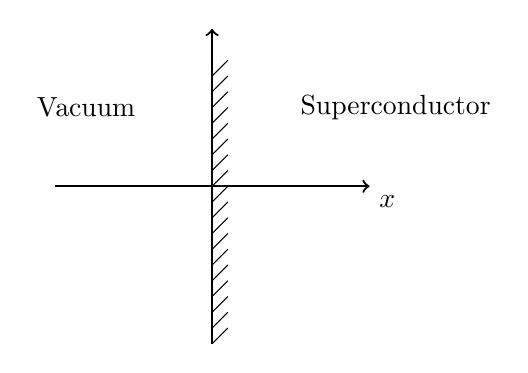
\begin{tikzpicture}[scale = 2]
\draw[thick, ->] (0,1) to (2,1);
\draw[thick, ->] (1,0) to (1, 2);
\foreach \y in {0,0.1,...,1.8} {
	\draw (1,\y) to (1.1, \y + 0.1);	
}
\node at (0.2,1.5) {Vacuum};
\node[anchor = west] at (1.5,1.5) {Superconductor};
\node[anchor = north west] at (2,1) {$x$};
\end{tikzpicture}
\caption{Semi-infinite superconductor}
\label{fig:semi_infinite_superconductor}
\end{figure}
Here, $\vb A = \vb A(x)$. At $x=0: \vb A(x=0) = \vb A_0$.
\begin{align} 
\dv[2]{\vb A}{x} &= \dfrac{1}{\lambda^2}\vb A  \\[2ex]
\implies \vb A(x) &= \vb A_0(x)\e^{-\frac{x}{\lambda}} \\[2ex]
\vb B(x) &= \curl{\vb A}
\end{align}
$B_i = \ep_{ijl}\partial_j A_l$. $j = x(=1)$ since there is only $x$-dependence. 
\begin{align*} 
B_y &= \ep_{213}\partial_x A_z =-\partial_xA_z = \frac1\lambda A_{0z}\e^{\frac{-x}{\lambda}} \\
B_z &= \ep_{312}\partial_x A_y =+\partial_xA_y = - \frac1\lambda A_{0y}\e^{\frac{-x}{\lambda}}
\end{align*}
Thus, 
\begin{equation} 
\vb B(x) = \vb B_0\e^{\frac{-x}{\lambda}}.
\end{equation}

\begin{figure}
	\centering
	\begin{tikzpicture}[scale = 0.75]
\begin{axis}[
axis lines = center,
x label style={ at={(axis description cs:1,0.05)}, anchor = west},
y label style={at={(axis description cs:0.45,1)},anchor=south},
ticks = none,
xlabel = $\Large x$,
ylabel = $\Large \vb B(x)$,
ymax = 1.3,
xmin =-1,
xmax=3
]

\addplot[thick,
domain=0:2, 
samples=100, 
color=blue]{exp(-x)};


\draw[->, thick] (axis cs:-0.3,0.3) to (axis cs:-0.3,0.9);
\node[anchor=east] at (axis cs:-0.3,0.6) {$\vb B_0$};
\node[anchor = south west] at (axis cs:0.6,0.5) {\Huge $\sim \e^{-\frac{x}{\lambda}}$};


\pgfplotsinvokeforeach{0,0.1,...,1.8} {
	\coordinate(a) at (axis cs:0,#1);
	\draw (a) -- ($(a) +(axis direction cs:0.1,0.1)$);	
};



\end{axis}
\end{tikzpicture}
\end{figure}
Now we see the physical meaning of $\lambda$: It is a characteristic length for how far a magnetic field penetrates a superconductor. It is referred to as the \underline{London penetration length.}
Thus, a magnetic field only exists withing a layer of thickness $\lambda$ from the surface of the superconductor. There is no magnetic field in the bulk of the superconductor. This is the Meissner-effect.
\begin{tcolorbox}[center, width = 0.5\textwidth]
	\centering
	Meissner-effect : $\lambda^{-1} >0$. \\[2ex]
	No Meissner-effect: $\lambda^{-1} = 0$. 
\end{tcolorbox}

The expression for $\lambda$ is
\begin{equation}
	\lambda = \left( \frac{m}{\mu_0n_s\left( e^* \right)^2} \right)^\frac{1}{2},
\end{equation}
a magnetic penetration length. $\lambda^{-1} > 0 $ if and only if $n_s >0$. $\lambda^{-1}=0$ otherwise. 
\underline{How does $n_s$ relate to $\Delta_k^\dagger$?}
$\Delta_k^\dagger$ originates with $b_k^\dagger = \ev{c_{-k\downarrow}c_{k\uparrow}}^\dagger$ which is the expectation value of the creation operator of a Cooper pair. Fourier-transformed to real-space it is the wavefunction $\psi(\vb r)$ of a Cooper-pair. $n_s \sim |\psi|^2$, thus $n_s \ne 0$ if and only if $\Delta_k\ne0$.\footnote{Says iff $\Delta_k = 0$ in the notes, which doesn't seem right.s}
Thus the onset of $\Delta_k$ for $T<T_C$ also means the onset of the Meissner-effect. 
\begin{tcolorbox}[center, width = 0.6\textwidth]
The onset of $\Delta_k$ at $T<T_C$ explains:
\begin{enumerate}[i)]
	\item loss of resistivity $\rho(T)$
	\item onset of Meissner-effect
\end{enumerate}
\end{tcolorbox}  
	
	% Week 11
	\section[Ginzburg-Landau]{Ginzburg-Landau theory of superconductors}

We have seen how the appearance of $\bd \neq 0$ leads to superconductivity, i.e. the expectation value of the creation operator of a Copper-pair obtains a nonzero value. Let us formulate this in real space and define a wave-function $\psi(\bm{r}) $ for Cooper-pairs. This wave-function then describes a superconductor. It is a local field where $|\psi|^2$ describes the local density of Copper-pairs. We now set up an energy for the superconductor in terms of this field $\psi(\bm{r})$. Since this field has charge $e^* (e^* = 2e$, where $e =$ electron charge) this matter field $\psi$ must be minimally coupled to a gauge-field $\bm{A}$ (where the magnetic field $B_\mu = \ep_{\mu\nu\lambda} \partial_\nu A_\lambda$), and the magnetic field density is given by $B_\mu B_\mu = (\grad \cross \bm{A} )^2$.


\begin{equation}
\begin{aligned}
\Ha  &= \frac{\hbar^2}{2m} \left |\left (-i\grad - e^*\bm{A}\right )\psi \right |^2 + \alpha |\psi|^2 + \frac{u}{2} |\psi|^4 + \frac{1}{2}(\grad \cross \bm{A} )^2 \\
\psi &= |\psi| \e^{i\theta}
\label{Ham_ginz_lan}
\end{aligned}
\end{equation}

This is a phenomenological model of superconductivity written down long before the advent of the BCS-theory, and with very limited knowledge of what $\psi(\bm{r})$ actually represented! However, after the BCS-theory was formulated, L.P: Gorkov \emph{derived} the GL-theory from the BCS-theory, and it became clear that

\begin{equation}
\Delta (\bm{r}) = \mathcal{F}^{-1}(\Delta_k) \iff \psi(\bm{r}).
\label{gap_fourrier}
\end{equation}

$\langle \psi(\bm{r}) \rangle$ then serves as an order-parameter of the superconductor.

\begin{itemize}
\item 1. term in equation $\Ha$: Kinetic enegy
\item 2. term in equation $\Ha$: ``Chemical potential''-term for Cooper-pairs
\item 3. term in equation $\Ha$: Contact repulsion term between Cooper-pairs .
\item 4. term in equation $\Ha$: Magnetic field energy.
\end{itemize}
Note that
\begin{equation}
\begin{aligned}
\alpha =& \alpha(T) \\
=& \alpha_0 (T - T_C^{MF}), 
\label{alpha}
\end{aligned}
\end{equation}
where $T_C^{MF}$ is a mean-field critical temperature of a superconductor. $T < T_C^{MF} \implies \alpha<0$ , and thus the ``chemical potential''-term makes it energetically advantageous to allow non-zero Cooper-pair density $|\psi|^2$.

\textbf{Landau theory:} Ignore kinetic term 

\begin{equation}
\Ha_L = \alpha |\psi|^2 + \frac{u}{2} |\psi|^4.
\label{H_L}
\end{equation}

Determine $|\psi|$ by minimizing $\Ha$ with respect to $|\psi|$:
\begin{equation}
\frac{\dd{\Ha_L}}{\dd|\psi|} = 0
\end{equation}

\begin{equation}
\begin{aligned}
\frac{\dd{\Ha_L}}{\dd|\psi|}  =&  2\alpha |\psi| + 2u|\psi|^3 \\
=& |\psi| (2\alpha + 2u |\psi^2) \\
i)\;|\psi|  =& 0 \\
ii)\; |\psi|  =& \left ( - \frac{\alpha}{u}\right )^\frac{1}{2}  
\label{alpha}
\end{aligned}
\end{equation}
Knowing that $|\psi| $ is real and non-negative, it is clear that

\begin{itemize}
\item $\alpha>0$: Only one real solution, $|\psi| = 0 \implies \Ha_L = 0$ (minimum)
\item  $\alpha<0$: Two real solutions: 
\begin{itemize}
\item$|\psi| = 0 \implies \Ha_L = 0$ \
\item$|\psi| = \sqrt{\frac{|\alpha|}{u}} \implies \Ha_L = \alpha \frac{|\alpha|}{u} + \frac{u}{2} \frac{|\alpha|^2}{u^2}$
\item $\Ha^{Min}_L = - \frac{|\alpha|^2}{2u} < 0$
\end{itemize}
\end{itemize}

$|\psi| =   \sqrt{\frac{|\alpha|}{u}} $ gives a lower energy  than $|\psi| =0$ so $|\psi| =   \sqrt{\frac{|\alpha|}{u}} $ is the correct solution for $\alpha<0$. $\Ha_L^{min} = -\frac{|\alpha|^2}{2u}$. $\Ha$ as a function of $|\psi|$ is plotted in the figure below.


\begin{figure}
\centering
\subfloat{
    \centering
    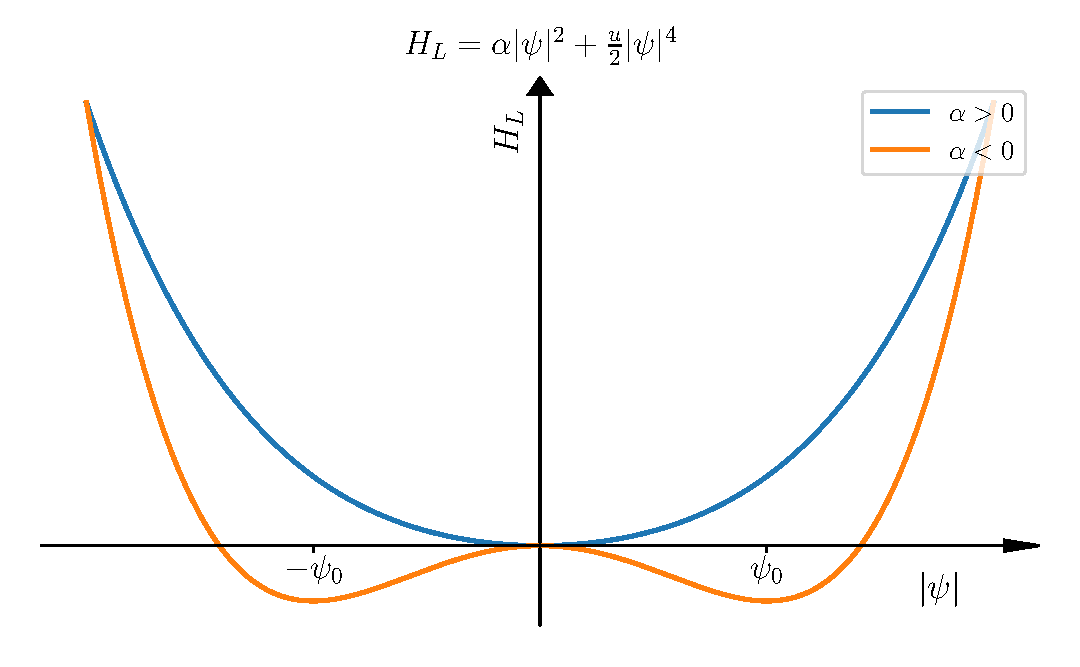
\includegraphics[width=\linewidth]{tex/pdf_files/H_L_1_D.pdf}
}
\caption{The Landau Hamiltonian, $\Ha_L$, as a function of $|\psi|$. Both signs of $\alpha$ are included, where $\alpha<0$, results in a minima in $\Ha_L$ at a nonzero $|\psi|$, denoted $\psi_0$.}
\label{fig:1D_H}
\end{figure}

For $\alpha<0$, we define 

\begin{equation}
\psi_0 = \sqrt{\frac{\alpha_0}{u}} (T_C^{MF} - T)^\frac{1}{2}.
\end{equation}

Observe that the critical exponent $\beta = \frac{1}{2}$ and that $\psi_0$ is a real number for $\alpha<0$, i.e. at $T<T_C^{MF}$. 


\newpage

Even though $\Ha_L$ only depends on the modulus of $\psi$, $\psi$ is still a complex number that can be written on the form $\psi=|\psi| \e^{i\theta}$. So we have the  energy landscape in the complex $\psi$-space as illustrated in the figure above.
\begin{figure}
\centering
\subfloat{
    \centering
    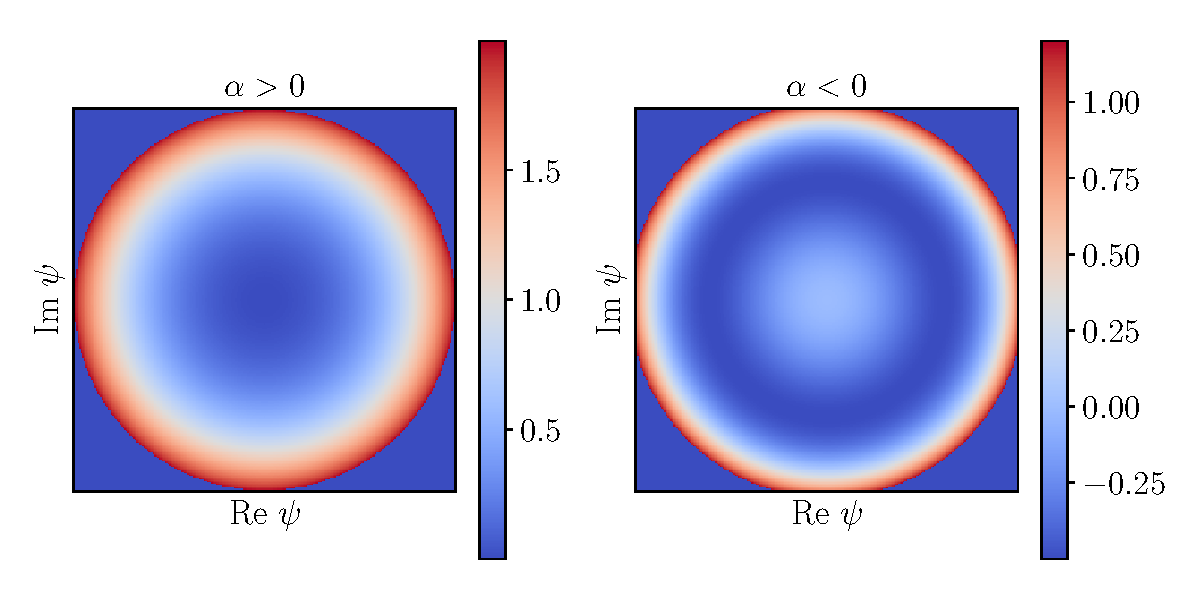
\includegraphics[width=\linewidth]{tex/pdf_files/H_L_2_D.pdf}
}
\caption{The Landau Hamiltonian, $\Ha_L$, as a function of the complex variable $\psi$. For $\alpha>0$ it is a simple paraboloid, monototonically increasing as the modulus of $\psi$ increases. However for $\alpha<0$, there exists a nonzero value of $|\psi|$ that yields a minima for $\Ha_L$.  It results in a Hamiltonian that bears a resemblence to a ''Sombrero hat''. Note that the minimum is only unique for the modulus, there is still a massively degenerate $\Ha_L$-minimum if the phase is included.}
\label{fig:1D_H}
\end{figure}

Note that from the ``Sombrero-hat''-picture, fluctuations in $\theta$ cost no energy in Landau-theory. On the other hand we see that fluctuations in $|\psi|$ around $\psi_0$ \emph{do} cost energy. 


Phase-fluctuations are ``massless''. Amplitude-fluctuations are ``massive''. 

Consider now also the kinetic energy and allow for phase-fluctuations and amplitude fluctuations. In other words, we allow 

\begin{equation}
\begin{aligned}
\psi =& (\psi_0 + \psi_1) \e^{i\theta}\\
\psi_0 =& \sqrt{\frac{|\alpha|}{u}} \; ; \; \psi_1 \; \mathrm{real}.
\label{psi_fluc}
\end{aligned}
\end{equation}


Consider first the Landau terms 

\begin{equation}
V(|\psi|) = \alpha |\psi|^2 + \frac{u}{2} |\psi|^4.
\label{V_psi}
\end{equation}

Expanding equation \cref{psi_fluc} to second order in $\psi_1$ for $\alpha<0$ yields


\begin{equation}
\begin{aligned}
V(|\psi|) & \\
=& \alpha (\psi_0^2 + 2\psi_0 \psi_1 + \psi_1^2) \\
+& \frac{u}{2} (\psi_0^4  \ 4\psi_0^3 \psi_1 + 6 \psi_0^2 \psi_1^2 + \mathcal{O}(\psi_1^3)) \\
=& \alpha_0 \psi_0^2 + \frac{u}{2} \psi_0^4 + 3u\psi_0^2\psi_1^2 + \alpha \psi_1^2 + \psi_1(2\alpha\psi_0 + 2u\psi_0^3), \mathrm{last}  \; \mathrm{term} = 0 \\
=& -\frac{\alpha^2}{2u} + \psi_1^2(\alpha - 3\alpha) \\
=& -\frac{\alpha^2}{2u} + 2|\alpha| \psi_1^2 \\
=& \Ha_L^{min} + 2\alpha \psi_1^2.
\label{psi_fluc_expansion}
\end{aligned}
\end{equation}

Consider next the kinetic energy term $\frac{\hbar^2}{2m} \left |\left (\frac{\grad}{i} - e^*\bm{A}\right )\psi \right |^2$

\begin{equation}
\begin{aligned}
& \left (-i\grad - e^*\bm{A}\right )(\psi_0 + \psi_1) \e^{i\theta} \\
=& -i\grad\psi_1  \e^{i\theta} - e^* \bm{A} \psi_1  \e^{i\theta} \\
+& (\grad \theta - e^* \bm{A} )(\psi_0 + \psi_1)  \e^{i\theta} \\
\simeq&  \left (-i\grad\psi_1 + (\grad \theta - e^* \bm{A} ) \psi_0 \right ) \e^{i\theta}.
\label{psi_fluc_expansion_kin}
\end{aligned}
\end{equation}
Here we have kept only terms that are linear in the fluctuations fields $\psi_1, \theta, \bm{A}$, since we will square the above expression to get the kinetic energy. 

\begin{equation}
\begin{aligned}
&\frac{\hbar^2}{2m} \left |\left (-i\grad - e^*\bm{A}\right )\psi \right |^2 \\
=& \frac{\hbar^2}{2m} \left [ (\grad \theta - e^* \bm{A} )^2 \psi_0^2 + (\grad \psi_1)^2 \right ]. \\
\Ha =& \Ha_L^{min} + \frac{\hbar^2 \psi_0^2}{2m} (\grad \theta - e^* \bm{A} )^2 \\
 +& \frac{\hbar^2}{2m} (\grad \psi_1)^2 + 2|\alpha| \psi_1^2 + + \frac{1}{2}({\grad} \cross \bm{A} )^2.
\label{H_fluc}
\end{aligned}
\end{equation}

When $\alpha<0$, we see that amplitude-fluctuations $\psi_1$ are always massive, even if we make $\grad \psi_1$ arbitrarly small. Fluctuations in the phase $\theta$, on the other hand are massless, which means they are much easier to excite, and can be made to have arbitrarly low energy by making $\grad \theta$ arbitrarly small. The same is true for the $(\grad \cross \bm{A})^2$-term. We therefore focus on the fluctuations in $\theta$ and $\bm{A}$, and discard the $\psi_1$-part.  Also discarding $\Ha_L^{min}$ and introducing 

\begin{equation}
\rho_s \equiv \frac{\hbar^2 \psi_0^2}{m},
\end{equation}

we have 

\begin{equation}
\Ha = \frac{\rho_s}{2}  (\grad \theta - e^* \bm{A} )^2 + \frac{1}{2}({\grad} \cross \bm{A} )^2.
\label{Ham_rel_fluc} 
\end{equation}

This is the theory descrbing the relevant fluctuations around the Landau mean-field theory.

By introducing the current 



\begin{equation}
\begin{aligned}
\bm{j} =& - \frac{\partial \Ha}{\partial (e^* \bm{A})} \\
=& \rho_s (\grad \theta - e^*\bm{A}),
\end{aligned}
\end{equation}

we can describe the current in the superconducting state with phase-ordering as 

\begin{equation}
\bm{j}  = -e^* \rho_s \bm{A}.
\label{j_super} 
\end{equation}

Equation \cref{j_super} is exactly the consitutive relation for $\bm{j}$ that we used in combination with Maxwell's equations to give the Meissner-effect.

Note that the theory has a local $U(1)$ gauge-invariance, $e^*\bm{A}' =  e^*\bm{A} - \grad \theta$. This transformation leaves $\Ha$ in equation \cref{Ham_rel_fluc} invariant

\begin{equation}
\Ha = \frac{\rho_s}{2} e^{*^2} {\bm{A}'}^2 + \frac{1}{2}({\grad} \cross \bm{A}')^2.
\label{Ham_rel_fluc_inv} 
\end{equation}

Note that it now appears that the gauge-field (photon) has acquired a mass 
\begin{equation}
m_A^2 \equiv  e^{*^2} \rho_s.
\end{equation}

Also note that we \emph{used} the $U(1)$ gauge-invariance to arrive at this conclusion. We thus have 

\begin{tcolorbox}
\begin{equation*}
\rho_s \neq 0 \iff \psi_0 \neq 0 \iff \mathrm{Cooper-pairs}.
\end{equation*}
\end{tcolorbox}

$\psi_0$ plays the role of a Higgs-field, and the presence of a Higgs condensate (in this case, a superconductor) gives the photon a \emph{mass $m_A$}. This leads to the Meissner-effect. 

The Ginzburg-Landau theory for a superconductor is identical in form to the Higgs-sector of the Standard model. 


\begin{tcolorbox}
The Bogoliubov quasiparticles described by $\eta_k$ and $\gamma_k$ in the BCS-theory are fermionic analogs of the so-called Higgs-particle. 
\end{tcolorbox}


	
\end{document}